%   this is a true latex file *-* 
% % NOTE: Check setting of the XXX (XXX=final, index, ...)  
%   variables below  to  
%   enable or suppress printing of an index or debugging statements 
%   Also note possible LaTeX incompatibilities with \printindex at the 
%   end of the document, which may become '\input standard.ind' on some 
%   systems which do not understand the '\printindex' command...

%              <=== declarations of logical vars XXX (XXX=final,index...)
\newif\iffinal
\newif\ifindex

%              <=== set the logicals (make them either \XXXtrue or \XXXfalse)
%              in the source us \ifXXX ... \else ... \fi
\finaltrue
\indextrue

%              various DOCUMENTSTYLE, depending on chosen environment
\ifindex
  \iffinal
    \documentclass[11pt,makeidx]{book}     % final version
    \usepackage{iaufwg}
    \usepackage{epsf}
    \usepackage{deluxetable}
  \else
    \documentclass[11pt,makeidx,showidx]{book}% index debug version
    \usepackage{iaufwg}
    \usepackage{epsf}
    \usepackage{deluxetable}
  \fi
\else
 \documentstyle[11pt]{book}                   % no index
    \usepackage{iaufwg}
\fi

%%%%%%%%%%%%%%%%%%%%%%%%%%%%%%%%%%%%%%%%%%%%%%%%%%%%%%%%%%%%%%%%%%%%%%%

\ifindex
  \makeindex
\fi

%%%%%%%%%%%%%%%%%%%%%%%%%%%%%%%%%%%%%%%%%%%%%%%%%%%%%%%

\begin{document} 

% FITS keywords, no argument.
\newcommand{\keyw}[1]{\hbox{{\tt #1}}}
% FITS keywords, single italicized argument.
\newcommand{\keyi}[2]{\hbox{{\tt #1\hspace{1pt}}{$#2$}\/}}
\newcommand{\CRPIX}[1]{\keyi{CRPIX}{#1}}
\newcommand{\CDELT}[1]{\keyi{CDELT}{#1}}
\newcommand{\CRVAL}[1]{\keyi{CRVAL}{#1}}
\newcommand{\CTYPE}[1]{\keyi{CTYPE}{#1}}
\newcommand{\CUNIT}[1]{\keyi{CUNIT}{#1}}
\newcommand{\NAXIS}[1]{\keyi{NAXIS}{#1}}
\newcommand{\CROTA}[1]{\keyi{CROTA}{#1}}
% FITS keywords, double italicized arguments.
\newcommand{\keyii}[3]{\hbox{{\tt #1\hspace{1pt}{$#2$}\_{$#3$}}\/}}
\newcommand{\PC}[2]{\keyii{PC}{#1}{#2}}
\newcommand{\CD}[2]{\keyii{CD}{#1}{#2}}
\newcommand{\PV}[2]{\keyii{PV}{#1}{#2}}
\newcommand{\PS}[2]{\keyii{PS}{#1}{#2}}
% FITS keyvalue.
\newcommand{\keyv}[1]{\hbox{{\tt #1}}}
% older ones
\newcommand{\PCij}{\PC{i}{j}}
\newcommand{\CDij}{\CD{i}{j}}
\newcommand{\Ci}{{\it a\/}}
\newcommand{\NN}[1]{\noalign{\noindent{#1}}\noalign{\vspace{4pt}}}

% Definitions for formatting keywords, indexed keywords, and alternate forms
\newcommand{\kwd}[1]{\texttt{#1}}
\newcommand{\kwdalt}[1]{\kwd{#1}\textit{a}}
\newcommand{\indxkw}[2]{\texttt{#1}\textit{#2}}
\newcommand{\indxkwdalt}[2]{\indxkw{#1}{#2}\textit{a}}
\newcommand{\dindxkw}[3]{\textit{#1}\/\indxkw{#2}{#3}}
\newcommand{\dindxkwalt}[3]{\dindxkw{#1}{#2}{#3}\textit{a}}

% A couple of defs from AASTeX
\newcommand\degr{\arcdeg}%
\newcommand\arcdeg{\mbox{$^\circ$}}%

\begin{titlepage}
\begin{center}

\vspace*{2.5cm}
{\LARGE \bf Definition of the Flexible Image Transport System ({\em FITS\/})} \\


\vspace{3.0cm}
{\em FITS\/} Standard \\

\vspace{0.8cm}
Version 3.0 \\

\vspace{0.6cm}
2008 July 10 \\

\vspace{4.0cm}
 {\em FITS\/} Working Group \\
Commission 5: Documentation and Astronomical Data \\
International Astronomical Union \\
{\tt http://fits.gsfc.nasa.gov/iaufwg/} \\

\end{center}
\end{titlepage}

%%%%%%%%%%%%%%%%%%%%%%%%%%%%%%%%%%%%%%%%%%%%%%%%%%%%%%%%%%%%%%%%%

                  %%% Cannot add \index here - no pagenumbers available
		  
\setcounter{page}{0}

\tableofcontents
\listoftables
%\listoffigures

%%%%%%%%%%%%%%%%%%%%%%%%%%%%%%%%%%%%%%%%%%%%%%%%%%%%%%%%%%%%%%%%%%%%%%%
%%%%%%%%%%%%%%%%%%%%%%%%%%%%%%%%%%%%%%%%%%%%%%%%%%%%%%%%%%%%%%%%%%%%%%%

\chapter{Introduction}
%   \addcontentsline{toc}{chapter}{Introduction}\markboth{}{}

\setcounter{page}{1}
\pagenumbering{arabic}

\begin{quote}
{\em An {\em archival format} must be utterly portable and
self-describing, on the assumption that, apart from the transcription
device, neither the software nor the hardware that wrote the data will
be available when the data are read.} 
{`Preserving Scientific Data on
our Physical Universe,' p.\ 60.} {Steering Committee for the Study on the
Long-Term Retention of Selected Scientific and Technical Records of the
Federal Government, [US] National Research Council, National Academy
Press 1995.}
\end{quote}

   This document, hereafter referred to as the `standard',  describes the
   Flexible Image Transport System ({\em FITS\/}) which is the standard
   archival data format for astronomical data sets. Although {\em FITS\/}
   was originally designed for transporting image data on magnetic tape
   (which accounts for the `I' and `T' in the name), the capabilities of
   the {\em FITS\/} format have expanded to  accommodate more complex data
   structures.   The role of {\em FITS\/} has also grown from simply a way to
   transport data between different  analysis software systems into the
   preferred format for data in astronomical archives, as well as the
   on-line analysis format used by many software packages.

   This standard is intended as a  formal codification of the {\em
   FITS\/} format  which has been  endorsed by the International
   Astronomical Union (IAU)\index{IAU} for the interchange of astronomical
   data \cite{iau83}. It is fully  consistent with all actions and endorsements of
   the  IAU {\em FITS\/} Working\index{IAUFWG} Group (IAUFWG) which was
   appointed by Commission 5 of the IAU to oversee further development of
   the  {\em FITS\/} format.   In particular, this standard defines the
   organization and content  of the header and data units for all 
   standard {\em FITS\/} data structures: the primary array, the random
   groups structure,  the image  extension, the  ASCII table extension,
   and the binary table extension.   It also specifies minimum  structural
   requirements and general principles governing the creation of new
   extensions.   For headers, it specifies the  proper syntax for keyword
   records and defines   required and  reserved keywords.  For
   data, it specifies character and numeric value representations and the
   ordering  of contents within the byte stream.  

   One important feature of the {\em FITS\/} format is that its structure,
   down to the bit level, is completely specified in documents (such as
   this standard), many of which have been published in refereed scientific
   journals.  Given these documents, which are readily  available in hard
   copy form in libraries around the world as well as in electronic form
   on the Internet, future researchers should be able to decode the stream
   of bytes in any {\em FITS\/} format data file.  In contrast, many other current
   data formats are only implicitly defined by the software that read and
   write the files.  If that software is not continually maintained so
   that it can be run on future computer systems, then the information
   encoded in those data files could be lost.

\section{Brief History of {\em FITS}}

  The {\em FITS\/} format evolved out of the
  recognition that a standard format was needed for 
  transferring astronomical images from one research institution to another.  
  The first prototype developments of a universal interchange format that would
  eventually lead to the definition of the {\em FITS\/} format began 
  in 1976 between Don Wells at KPNO and  Ron Harten at the Netherlands 
  Foundation for Research in Astronomy (NFRA).  This need for an image
  interchange format was raised at a meeting of the Astronomy
  section of the U.S. National Science Foundation in January 1979, which led 
  to the formation of a task force to work on the problem.  Most of the
  technical details of the first basic {\em FITS\/} agreement (with files
  consisting of only a primary header followed by a data array) were
  subsequently developed by Don Wells and Eric Greisen (NRAO) in March 1979.
  After further refinements, and successful image interchange tests 
  between observatories that used widely
  different types of computer systems, the first papers that defined the
  {\em FITS\/} format were published in 1981 \cite{wells81, greisen81}.   The {\em FITS\/} format
  quickly became the defacto standard for data interchange 
  within the astronomical community  (mostly on 
  9-track magnetic tape at that time) and  was officially
  endorsed by the IAU \index{IAU} in 1982 \cite{iau83}.  Most national and international
  astronomical projects and organizations subsequently adopted the {\em FITS\/} format
  for distribution and archiving of their scientific data products.
  Some of the highlights in the developmental history of {\em FITS} are shown in Table \ref{t:hist}

\begin{deluxetable}{ll}
\tabletypesize{\small}
%\tabletypesize{\scriptsize}
%\tabletypesize{\tiny}
\tablecolumns{2}
\tablewidth{0pt}
\tablecaption{Significant milestones in the development of {\em FITS}.
\label{t:hist}}
\tablehead {
\colhead{Date} & \colhead{Milestone}  
}
%
\startdata
      1979 & Initial {\em FITS\/} Agreement and first interchange of files \\
      1981 & Published original (single HDU) definition \cite{wells81} \\
      1981 & Published random groups definition \cite{greisen81} \\
      1982 & Formally endorsed by the IAU \cite{iau83} \\
      1988 & Defined rules for multiple extensions \cite{grosbol88} \\
      1988 & IAU {\em FITS\/} Working Group (IAUFWG) established \\
      1988 & Extended to include ASCII table extensions \cite{harten88} \\
      1988 & Formal IAU approval of ASCII tables \cite{iau88} \\
      1990 & Extended to include IEEE floating-point data \cite{wells90} \\
      1994 & Extended to multiple {\tt IMAGE} array extensions \cite{ponz94}\\
      1995 & Extended to binary table extensions \cite{cotton95} \\
      1997 & Adopted 4-digit year date format \cite{bunclark97}\\
      2002 & Adopted conventions for celestial world coordinates \cite{greisen02, calabretta02} \\
      2004 & Adopted MIME types for {\em FITS\/} data files \cite{rfc4047} \\
      2005 & Extended to support variable-length arrays in binary tables \\
      2005 & Adopted conventions for spectral coordinate systems \cite{greisen06} \\
      2005 & Extended to include 64-bit integer data type\\ 
\enddata
\end{deluxetable}


\newpage
\section{Version History of this Document}

The fundamental definition of the {\em FITS\/} format was originally
contained in a series of published papers \cite{wells81, greisen81, 
grosbol88, harten88}. As
{\em FITS\/} became more widely used, the need for a 
single document to unambiguously define the requirements of
the {\em FITS\/} format became apparent.  
In 1990, the NASA Science Office of Standards and Technology
(NOST) at the Goddard Space Flight Center provided funding 
for a technical panel to develop the first version of this standard
document.   As shown in Table \ref{t:docs}, the NOST panel produced several
draft versions, culminating in the first NOST standard document, NOST 100-1.0,
in 1993.  Although this document was developed under a NASA accreditation process, 
it was subsequently formally approved by the IAUFWG, \index{IAUFWG} which is the international
control authority for the {\em FITS\/} format.  The small update to the standard
in 1995 (NOST 100-1.1) added a recommendation on the physical units of header
keyword values.

\begin{deluxetable}{lll}
\tabletypesize{\small}
%\tabletypesize{\scriptsize}
%\tabletypesize{\tiny}
\tablecolumns{3}
\tablewidth{0pt}
\tablecaption{Version history of the standard.
\label{t:docs}}
\tablehead {
\colhead{Version} & \colhead{Date} & \colhead{Status}  
}
%
\startdata
NOST 100-0.1   & 1990 December & 1st Draft Standard  \\ 
NOST 100-0.2   & 1991 June    & 2nd Revised Draft Standard  \\ 
NOST 100-0.3   & 1991 December & 3rd Revised Draft Standard  \\
NOST 100-1.0   & 1993 June & NOST Standard  \\
NOST 100-1.1   & 1995 September & NOST Standard  \\ 
NOST 100-2.0   & 1999 March & NOST Standard  \\ 
IAUFWG 2.1     & 2005 April & IAUFWG Standard  \\ 
IAUFWG 2.1b    & 2005 December & IAUFWG Standard  \\ 
IAUFWG 3.0     & 2008 July  & IAUFWG Standard  \\ 
\enddata
\end{deluxetable}


The NOST technical panel was convened a second time to make further updates
and clarifications
to the standard, resulting in the NOST 100-2.0 version that was approved by 
the IAUFWG in 1999 and published in 2001 \cite{hanisch01}.  In 2005, the IAUFWG formally approved the variable-length
array convention in binary tables, and a short time later approved support for the 
64-bit integers data type.  New versions of the standard were released to
reflect both of these changes (versions IAUFWG 2.1 and IAUFWG 2.1b).

Most recently, the IAUFWG \index{IAUFWG} appointed
its own technical panel in early 2007 to consider further modifications and updates
to the standard.  The changes proposed by this panel, which were ultimately approved
by the IAUFWG after a formal public review process, are shown in this 
3.0 version of the document.

The latest version of the standard, as well as other information about
the {\em FITS\/} format, can be obtained from the {\em FITS\/} Support
Office web site at
\newline {\tt http://fits.gsfc.nasa.gov}.

\newpage
\section{Acknowledgments}


The members of the 3 technical panels that produced this standard are shown below.  

\begin{table}[h]
\begin{center}
\begin{tabular}{ll} \\
\vspace{-5pt} \\
\multicolumn{2}{l}{\bf First technical panel, 1990 -- 1993} \\ 
  	 Robert J. Hanisch (Chair)  &  Space Telescope Science Institute \\
         Lee E. Brotzman  &  Hughes STX \\
         Edward Kemper  & Hughes STX \\
         Barry M. Schlesinger   & Raytheon STX \\
         Peter J. Teuben  & University of Maryland \\
         Michael E. Van Steenberg  & NASA Goddard Space Flight Center \\
         Wayne H. Warren Jr.  &  Hughes STX \\
         Richard A. White &  NASA Goddard Space Flight Center \\
       
\\
\multicolumn{2}{l}{\bf Second technical panel, 1994 -- 1999} \\ 

  	 Robert J. Hanisch (Chair)  &  Space Telescope Science Institute \\
         Allen Farris   & Space Telescope Science Institute \\
         Eric W. Greisen  & National Radio Astronomy Observatory \\
         William D. Pence   & NASA Goddard Space Flight Center \\
         Barry M. Schlesinger    & Raytheon STX \\
         Peter J. Teuben  & University of Maryland \\
         Randall W. Thompson  & Computer Sciences Corporation \\
         Archibald Warnock   & A/WWW Enterprises \\
\\	     
\multicolumn{2}{l}{\bf Third technical panel, 2007} \\ 

         William D. Pence (Chair)  & NASA Goddard Space Flight Center \\
         Lucio Chiappetti  & IASF Milano, INAF, Italy \\
         Clive G. Page  & University of Leicester, UK \\
         Richard Shaw  & National Optical Astronomy Observatory \\
         Elizabeth Stobie  & University of Arizona \\
	     
\end{tabular}
\end{center}
\end{table}   


%%%%%%%%%%%%%%%%%%%%%%%%%%%%%%%%%%%%%%%%%%%%%%%%%%%%%%%%%%%%%%%%%%%%%%%
%%%%%%%%%%%%%%%%%%%%%%%%%%%%%%%%%%%%%%%%%%%%%%%%%%%%%%%%%%%%%%%%%%%%%%%

\chapter{Definitions, Acronyms, and Symbols}
\label{s:def}

\section{Conventions used in this document}

Terms or letters set in {\tt Courier font} represent literal strings 
that appear in {\em FITS\/} files.  In the case of keyword names, such as
`{\tt NAXISn}', the lower case letter represents a positive integer  index number,
generally in the range 1 to 999.
The emphasized words {\em must, shall, should, may, recommended,} and {\em optional} 
in this document are to be interpreted as 
described in IETF standard, RFC 2119 \cite{rfc2119}.

\section{Defined Terms}

\begin{description}
\item[\hbox{\tt\char`\ }] Used to designate an ASCII space character.
\item[ANSI] American National Standards\index{ANSI}
    Institute.
\item[Array]  A sequence of data values. This sequence 
     corresponds to the elements in a rectilinear, n-dimension matrix 
     ($1 \leq n \leq 999$, or $n = 0$ in the case of a null array).
\item[Array value] The\index{array value} value of an element of an array 
     in a {\em FITS\/} file, without the application of the 
     associated linear transformation to derive the
     physical\index{physical value} value.
\item[ASCII] American National Standard Code 
             for Information\linebreak[1] Interchange.
\item[ASCII character] Any\index{ASCII character} 
      member of the 7-bit ASCII character set. 
\item[ASCII digit] One of the 10 ASCII characters `0' through `9'
      which are represented by decimal character codes 48 through 57
      (hexadecimal 30 through 39).
\item[ASCII NULL] The ASCII character\index{NULL, ASCII} that has all 8 
      bits set to zero.
\item[ASCII space] The ASCII character for space
      which is represented by decimal 32 (hexadecimal 20).
\item[ASCII text] The restricted set of ASCII characters\index{ASCII text} 
      decimal 32 through 126 (hexadecimal 20 through 7E).
\item[Basic {\em\bf FITS}] The {\em FITS\/} 
      structure\index{FITS structure} consisting of
      the primary header\index{primary header} followed by a single
      primary\index{primary data array} data array. This is also known
      as  Single Image {\em FITS\/} (SIF), as opposed to 
      Multi-Extension {\em FITS\/} (MEF) files that contain 
      one or more extensions following the primary HDU.
\item[Big endian]  The numerical data format used in {\em FITS\/} files 
in which the most significant byte of the value is stored first followed by the
remaining bytes in order of significance.
\item[Bit] A single binary digit.
\item[Byte] An ordered sequence of eight consecutive bits treated as a single entity.
\item[Card image]  An obsolete term for an 80-character keyword record
     derived from the 80 column punched computer cards that were prevalent
     in the 1960s and 1970s.
\item[Character string] A sequence of 1 or more of the restricted set of ASCII text characters,
    decimal 32 through 126 (hexadecimal 20 through 7E). \index{character string}
\item[Conforming extension] An extension whose keywords and
         organization\index{conforming extension}
         adhere to the requirements for conforming extensions defined 
         in \S\ref{s:genext} of this 
         standard.\index{extension, conforming}
\item[Data block]  A 2880-byte {\em FITS\/} block containing data described by the
         keywords in the associated header of that HDU.
\item[Deprecate]  To express disapproval of. This term\index{deprecate} is used 
        to refer to obsolete structures that {\em should not} be used in
	new {\em FITS\/} files but which {\em shall} remain valid indefinitely.
\item[Entry] A single value in an ASCII table or  binary table standard extension.
\item[Extension] A\index{extension} {\em FITS\/} HDU 
     appearing\index{HDU, extension} after the primary HDU in a 
     {\em FITS\/} file.
\item[Extension type name] The value of the {\tt XTENSION}
   keyword\index{XTENSION}, used to identify
   the type\index{extension type name} of the extension. 
\item[Field] A component of a larger entity, such as a keyword record or
    a row of an  ASCII table or binary table standard extension.  
    A field in a table extension row consists of a set of zero or more table 
     entries collectively described by a single format.
\item[File] A sequence of one or more records terminated by an end-of-file
             indicator appropriate to the medium.
\item[{\em\bf FITS}] Flexible Image Transport System.
\item[{\em\bf FITS} block] A sequence of 2880 8-bit bytes aligned on 2880 
byte boundaries in the {\em FITS\/} file, most commonly either a header 
block or a data block.  Special records are another infrequently used type
of {\em FITS\/} block.    This block length was chosen because it is evenly
divisible by the byte and word lengths of all known computer systems at the time
{\em FITS\/} was developed in 1979.
\item[{\em\bf FITS} file] A file with a format that conforms to the 
            specifications in this document.
\item[{\em\bf FITS} structure] One\index{FITS structure} of the 
               components of a {\em FITS\/} file: 
               the primary\index{HDU, primary} HDU, 
               the random groups\index{random groups} records, an 
               extension\index{extension}, or, collectively, 
               the special records\index{special records} following 
               the last extension.
\item[{\em\bf FITS} Support Office] The {\em FITS\/} information
web site that is maintained by the IAUFWG and is currently hosted
at {\tt http://fits.gsfc.nasa.gov}.
\item[Floating-point] A computer representation of a real number.
\item[Fraction]The field of the mantissa\index{mantissa}
              (or significand) of a floating-point number that lies to
              the right of its implied binary point.   
\item[Group parameter value] The\index{group parameter value} 
     value of one of the parameters preceding a group in the random groups
     structure, without the application of the 
     associated linear transformation.
\item[HDU] Header and Data Unit. A data structure 
       consisting of a
       header and the data the header describes. Note that an\index{HDU}
       HDU {\em may} consist entirely of a header with no data blocks.
\item[Header] A series of keyword records organized within 
       one or more 
       header blocks that describes structures 
       and/or data which follow it in the {\em FITS\/} file.
\item[Header block]  A 2880-byte {\em FITS\/} block containing a sequence of thirty-six 
80-character keyword records. 
\item[Heap] The supplemental data area following the main data table in 
       a\index{heap} binary table standard extension.
\item[IAU] International Astronomical\index{IAU} Union.
\item[IAUFWG] \index{IAUFWG}
       International Astronomical Union {\em FITS\/} Working Group.
\item[IEEE] Institute of Electrical and 
        Electronic Engineers.
\item[IEEE NaN] IEEE Not-a-Number\index{IEEE NaN} 
        value; used to represent undefined floating-point values
	in {\em FITS\/} arrays and binary tables.
\item[IEEE special values] Floating-point number byte patterns that have
       a special, reserved meaning, such as
        $-0$, $\pm \infty$, $\pm$underflow, $\pm$overflow, $\pm$denormalized,
        $\pm$ NaN.\index{IEEE special values} (See Appendix \ref{s:IEEE754}).
\item[Indexed keyword] A\index{keyword, indexed} keyword name that is 
       of the form of a fixed root with an appended positive integer index number.
\item[Keyword name] The first eight bytes of a keyword record which
contain the ASCII name of a metadata quantity (unless it is blank).
\item[Keyword record] An 80-character record in a header block
consisting of a keyword name in the first 8 characters followed by an {\em optional}
value indicator, value and comment string.  
The keyword record {\em shall} be composed only of the
restricted set of ASCII text characters ranging from decimal 32 to 126 
(hexadecimal 20 to 7E).
\item[Mandatory keyword] A\index{keyword, required} keyword that {\em must} 
   be used in all {\em FITS\/} files or a keyword required 
   in conjunction with particular\index{FITS structure} {\em FITS\/}
   structures.
\item[Mantissa] Also\index{mantissa} known as\index{significand}
                significand. The component of an IEEE floating-point
                number consisting of an explicit or implicit leading bit
                to the left of its implied binary point and a fraction
                field to the right.          
\item[MEF] Multi-Extension {\em FITS\/}, i.e., a {\em FITS} file containing a primary
    HDU followed by one or more extension HDUs.
\item[NOST] NASA/Science Office of Standards and 
       Technology.
\item[Physical value] The\index{physical value} value in physical 
   units\index{units} represented by an element
   of an array and possibly derived from 
   the array value\index{array value}
   using the associated, but {\em optional}, linear transformation.
\item[Pixel] Short for `Picture element';  a single location within an array.
\item[Primary data array] The\index{primary data array}
   data array contained in the\index{HDU, primary} primary HDU.
\item[Primary HDU] The first HDU in a {\em FITS\/} file.
\item[Primary header] The\index{primary header} first header 
   in a {\em FITS\/} file, containing information on the 
   overall contents of the file (as well as on the
   primary data array, if present).
\item[Random Group] A {\em FITS\/} structure consisting of a collection
of `groups', where a group consists of a subarray of data and a
set of associated parameter values.  Random groups are deprecated for
any use other than for radio interferometry data.
\item[Record] A sequence of bits treated as a single logical entity.

\item[Repeat count] The\index{repeat count} number of values 
    represented in a field in a binary table\index{binary table} standard extension.
\item[Reserved keyword] An\index{keyword, reserved} {\em optional} keyword 
   that {\em must} be used only in the manner defined in this standard.
\item[SIF] Single Image {\em FITS\/}, i.e., a {\em FITS\/} file containing only a primary
    HDU, without any extension HDUs.  Also known as Basic {\em FITS\/}.
\item[Special records] A series of one or more {\em FITS\/} blocks 
   following the last HDU \index{special records}
   whose internal structure does not otherwise conform to that for
   the primary HDU or to that specified for a conforming 
   extension\index{conforming extension} in
   this standard.  Any use of special records requires approval from
   the IAU FITS Working Group.
\item[Standard extension] A\index{standard extension}
     conforming\index{conforming extension} 
     extension\index{extension, conforming} 
   whose\index{extension, standard} header and data 
   content are completely specified in \S\ref{s:exts} of this standard, namely,
   an image extension, an ASCII table extension, or a binary table extension.
\end{description}

%%%%%%%%%%%%%%%%%%%%%%%%%%%%%%%%%%%%%%%%%%%%%%%%%%%%%%%%%%%%%%%%%%%%%%%%%%%%%%%%
%%%%%%%%%%%%%%%%%%%%%%%%%%%%%%%%%%%%%%%%%%%%%%%%%%%%%%%%%%%%%%%%%%%%%%%%%%%%%%%%


\chapter{{\em FITS\/} File Organization}
  \label{s:org}

  \section{Overall File Structure}

   A {\em FITS\/} file {\em shall} be composed of the following {\em FITS\/} 
   structures\index{FITS structure}, in the 
   order\index{order, {\em FITS\/} structures}
   listed:
   \begin{itemize}
   \item Primary header and data unit (HDU)\index{HDU, primary}
   \item Conforming Extensions\index{conforming extension}
   ({\em optional})\index{extension, conforming}
   \item Other special records ({\em optional}, restricted)\index{special records}
   \end{itemize}
\noindent
   A {\em FITS\/} file composed of only the primary HDU is sometimes referred to
   as a Basic {\em FITS\/} file, or a Single Image {\em FITS\/} (SIF) file, and a
   {\em FITS\/} file  containing one or more extensions following the primary HDU
   is sometimes referred to as a Multi-Extension {\em FITS\/} (MEF) file. 
   
   Each {\em FITS\/} structure\index{FITS structure} {\em shall}  consist of an
   integral number of {\em FITS\/} blocks which are each 2880 bytes (23040 bits)
   in length. The primary HDU\index{HDU, primary} {\em shall} start  with the
   first {\em FITS\/} block of the {\em FITS\/} file.  The first {\em FITS\/}
   block of each subsequent  {\em FITS\/} structure\index{FITS structure} {\em
   shall} be  the {\em FITS\/} block immediately  following the last {\em FITS\/}
   block of the preceding {\em FITS\/} structure.  

This standard does not impose a limit on the total size of 
a {\em FITS\/} file, nor on the size of an individual HDU within 
a {\em FITS\/} file. Software packages that read or write data 
according to this standard could be limited, however, in the size of
files that are supported. In particular, some software systems have 
historically only supported files up to $2^{31}$ bytes in size 
(approximately $2.1\times10^9$ bytes). 

  \section {Individual {\em FITS\/} Structures} 
   The primary HDU and every
   extension\index{extension}  HDU\index{HDU, extension} {\em shall} consist
   of 1 or more 2880-byte header blocks immediately followed by an {\em optional}
   sequence of associated 2880-byte data blocks. The header blocks {\em shall}
   contain only the restricted set of ASCII\index{ASCII text} text characters,
   decimal 32 through 126 (hexadecimal 20 through 7E).  The ASCII control
   characters with decimal values less than 32 (including the null, tab,
   carriage return, and line feed characters), and the delete character
   (decimal 127 or hexadecimal 7F) {\em must not} appear anywhere within a header block.  

  \section{Primary Header and Data Unit}
   The first component of a {\em FITS\/} file {\em shall} be the 
   primary HDU which always contains the primary header and 
   {\em may} be followed by
   the primary data\index{primary data array}
   array. If the primary data array has zero length, as
   determined by the values of the {\tt NAXIS} 
   and\index{NAXIS} {\tt NAXISn} keywords\index{NAXISn}
   in the primary header (\S\ref{s:pman}), then the primary HDU
   {\em shall} contain no data blocks.
  
   \subsection{Primary Header} The header of a primary 
   HDU\index{HDU, primary} {\em shall} consist of  one or more header blocks, each
   containing a series of 80-character keyword 
   records\index{keyword record} containing only the restricted set of 
   ASCII\index{ASCII text}
   text characters.  Each 2880-byte header  block contains 36 keyword
   records.  The last header block {\em must} contain the {\tt END} keyword
   (defined in \S\ref{s:pman}) which marks the logical end of the header. 
   Keyword records without information  (e.g., following the
   {\tt END} \index{END} keyword) {\em shall} be
   filled\index{fill} with ASCII spaces (decimal 32 or hexadecimal 20).

   \subsection{Primary Data Array}
   The \label{s:pdata} primary\index{primary data array} data array, if
   present, {\em shall} consist of a  single data array with from 1 to
   999~dimensions (as specified by the {\tt NAXIS} keyword defined in
   \S\ref{s:pman}).   The random groups convention in the
   primary data array is a  more complicated structure and is discussed
   separately in \S\ref{s:Rgrp}.  The entire array of data values are
   represented by a continuous stream of  bits starting with the first
   bit of the first data block. Each data value {\em shall} consist of a
   fixed number of bits that is determined by the value of the {\tt
   BITPIX} keyword (\S\ref{s:pman}).  Arrays of more than
   one dimension {\em shall} consist of
   a sequence such that the index along axis 1 varies most rapidly,
   that along axis~2 next most rapidly, and those along subsequent axes
   progressively less rapidly, with that along axis {\tt m}, where {\tt
   m} is the value  of {\tt NAXIS}\index{NAXIS}, varying least
   rapidly.    There is no space or any other special character between
   the last value on a row or plane and the first value on the  next row or plane
   of a multi-dimensional array. 
   Except for the\index{array, multi-dimensional}
   location of the first element, the array structure is independent of 
   the {\em FITS\/} block structure.
   This storage  order
   is shown schematically in  Figure \ref{f:array} and is
   the same order as in multi-dimensional arrays in the 
   Fortran \index{Fortran} programming language \cite{iso04}.
   The index count along each axis {\em shall} begin 
   with 1 and increment by 1 up to the value of 
   the {\tt NAXISn}\index{NAXISn} keyword (\S\ref{s:pman}). 
\begin{figure}[t]
 \begin{center}
\begin{tabular}{l} \\
          A(1, 1, \ldots, 1), \\ 
          A(2, 1, \ldots, 1), \\ 
          \hspace{0.5in}\vdots, \\ 
          A({\tt NAXIS1}, 1, \ldots, 1), \\
          A(1, 2, \ldots, 1), \\ 
          A(2, 2, \ldots, 1), \\ 
          \hspace{0.5in}\vdots, \\ 
          A({\tt NAXIS1}, 2, \ldots, 1), \\
          \hspace{0.5in}\vdots,          \\ 
          A(1, {\tt NAXIS2}, \ldots, {\tt NAXISm}), \\  
          \hspace{0.5in}\vdots,  \\ 
          A({\tt NAXIS1}, {\tt NAXIS2}, \ldots, {\tt NAXISm}) \\
\end{tabular}
\end{center}
\caption[Array data sequence]
   {Arrays of more than one dimension {\em shall} consist of a sequence 
   such that the index along axis 1 varies most rapidly and 
   those along subsequent axes progressively less rapidly. }
\label{f:array}

\end{figure}

   If the data array does not fill the final data block, the
   remainder of the data block {\em shall} be filled by setting all bits to zero.  
   The individual data values {\em shall} be stored in big-endian byte order such
   that the byte containing the most significant bits of the value appears
   first in the  {\em FITS\/} file, followed by the remaining bytes, if any,
   in decreasing order of significance.
  
  \section{Extensions}
  
   \subsection{Requirements for Conforming Extensions}
    \label{s:genext}  
   All extensions\index{extension}, 
   whether or not further described in this standard, {\em shall}
   fulfill the following requirements to be in conformance with
   this {\em FITS\/} standard. 
   New extension types {\em should} be created only when the organization
   of the information is such that it cannot be handled by one of 
   the existing extension types.  A {\em FITS\/} file that contains
   extensions is commonly referred to as a multi-extension {\em FITS\/} (MEF)
   file.
   
   \subsubsection{Identity}
   \label{s:idy}
   Each extension\index{conforming extension}
   type\index{extension, conforming} 
   {\em shall} have a unique type name, 
   specified in the\index{extension type name}
   header by the {\tt XTENSION} keyword (\S\ref{s:conf}).
   To preclude conflict, extension type names {\em must} be 
   registered\index{extension registration}
   with the\index{IAUFWG} IAUFWG\@.  The current list of
   registered extensions is given in Appendix \ref{s:resname}.
   An up to date list is also maintained on the {\em FITS\/} 
   Support Office web site.
  
   \subsubsection{Size Specification}
   The total number of bits in the data of each extension
   {\em shall} be specified in the header for that extension, in the
   manner prescribed in \S\ref{s:conf}.
  
   \subsection{Standard Extensions}
   A standard\index{standard extension} 
   extension\index{extension, standard} is a 
   conforming\index{conforming extension}
   extension\index{extension, conforming} whose
   organization and content are completely specified in  
   \S\ref{s:exts} of this standard.
   Only one extension format
   {\em shall} be approved for each type of data organization.  
  
   \subsection{Order of Extensions}
   An extension {\em may} follow the primary HDU\index{HDU, primary}  
   or another conforming\index{conforming extension}
   extension\index{extension, conforming}. 
   Standard\index{standard extension} 
   extensions\index{extension, standard} 
   and other conforming extensions {\em may} appear 
   in any order\index{order, extensions}
   in a {\em FITS\/} file.
  
  \section{Special Records (Restricted Use)}
   Special records are 2880-byte {\em FITS\/} blocks following the last HDU
   of the {\em FITS\/} file that have an unspecified structure that does not
   meet the requirements of a conforming extension. The first 8
   bytes of the special records {\em must not} contain\index{special records} the
   string\index{XTENSION} `\verb+XTENSION+'.  It is {\em recommended} that they
   do not contain the string\index{SIMPLE}  
   `\verb*+SIMPLE  +'. The contents of special records are not otherwise 
   specified by this standard.  

   Special records were originally designed as a way for the {\em FITS\/}
   format to evolve by allowing new {\em FITS\/} structures to be implemented.  
   Following the development of conforming extensions, which provide a general
   mechanism for storing different types of data structures in {\em FITS\/} format in
   a well defined manner, the need for other new types of {\em FITS\/} data
   structures has been greatly reduced.  Consequently, further use of special
   records is restricted and requires the approval of the IAU FITS Working 
   Group.\index{IAUFWG}

   \section{Physical Blocking}
   \label{s:PhysBlk}  
    \subsection{Bitstream Devices}     
     \label{s:BitDev}
For bitstream devices, including but not restricted to  logical file systems, 
{\em FITS\/} files {\em shall} be interpreted as a sequence  of 1 or more 2880-byte
{\em FITS\/} blocks, regardless of the physical blocking structure of the
underlying recording media.  When writing a {\em FITS\/} file on  media with a
physical block size unequal to the 2880-byte {\em FITS\/} block  length, any
bytes remaining in the last physical block following  the end of the {\em
FITS\/} file {\em should} be set to zero.  Similarly, when reading  {\em FITS\/}
files on such media, any bytes remaining in the last physical block following 
the end of the {\em FITS\/} file {\em shall} be disregarded. 

    \subsection{Sequential Media}

The {\em FITS\/} format was originally developed for writing files
on sequential magnetic tape devices.  The following rules on how to write
to sequential media \cite{grosbol94} are now irrelevant to most current data storage
devices.

If physically possible, {\em FITS\/} files {\em shall} be written on sequential 
media in blocks that are from 1 to 10 integer multiples of
2880-bytes in length.  If this is not possible, the {\em FITS\/} file {\em shall}
be written as a bitstream using the native block size of the sequential device.
Any bytes remaining in the last block following  the end of the 
{\em FITS\/} file {\em shall} be set to zero.

When reading {\em FITS\/} files on sequential media, any files 
shorter than 2880 bytes in length (e.g., ANSI tape labels)
are not considered part of the {\em FITS\/} files and {\em should} be disregarded.

  \section{Restrictions on Changes}
  \label{s:Restrict}
   Any structure that is a valid {\em FITS\/} 
   structure\index{FITS structure} {\em shall} remain 
   a valid {\em FITS\/} structure at all future times. 
   Use of certain 
   valid {\em FITS\/} structures {\em may} be 
   deprecated\index{deprecate} by this or 
   future {\em FITS\/} standard documents.
     
%%%%%%%%%%%%%%%%%%%%%%%%%%%%%%%%%%%%%%%%%%%%%%%%%%%%%%%%%%%%%%%%%%%%%%%%%%%%%%%%
%%%%%%%%%%%%%%%%%%%%%%%%%%%%%%%%%%%%%%%%%%%%%%%%%%%%%%%%%%%%%%%%%%%%%%%%%%%%%%%%

\chapter{Headers}
  \label{s:head}
  
 The first 2 sections of this chapter define the structure and content of header 
 keyword records.  This is followed in \S\ref{s:Units} with recommendations
 on how physical units should be expressed.  The final section defines the
 mandatory and reserved keywords for primary arrays and conforming extensions.
  
  \section{Keyword Records}
  
   \subsection{Syntax}
   Each 80-character header keyword record\index{keyword record}
   {\em shall} consist of a keyword name, a value indicator 
   (only required if a value
   is present), an {\em optional} value, and an {\em optional} comment.  Except
   where specifically stated otherwise\index{order, keyword}
   in this standard, keywords {\em may} appear in any order.
   It is {\em recommended} that the order of the keywords in 
   {\em FITS\/} files be preserved during data processing operations 
   because the designers of the {\em FITS\/} file may have used conventions 
   that attach particular significance to the order of certain keywords
   (e.g., by grouping sequences of {\tt COMMENT} keywords
   at specific locations in the header, or appending {\tt HISTORY} 
   keywords in chronological order of the data processing steps).

A formal syntax, giving a complete definition of the syntax of
{\em FITS\/} keyword records, is given in Appendix \ref{s:FormSyn}.  
It is intended as an aid in interpreting the text defining the standard.
  
   \subsection{Components}
  
   \subsubsection{Keyword name (bytes 1 through 8)}
       \label{s:keyw}
The keyword name {\em shall} be a left justified, 8-character, 
space-filled, ASCII\index{fill} string with no embedded spaces.  All 
digits 0 through 9 (decimal ASCII codes 48 to 57, or hexadecimal 30 to 39) and 
upper case\index{case sensitivity}
Latin alphabetic characters\index{keyword, valid characters}
{\tt `A'} through {\tt `Z'} (decimal 65 to 90 or hexadecimal 41 to 5A) are 
permitted; lower case characters {\em shall not} be used.  The 
underscore\index{underscore}
({\tt `\_'}, decimal 95 or hexadecimal 5F) and 
hyphen\index{hyphen}
({\tt `-'}, decimal 45 or hexadecimal 2D) are also permitted.  No other characters
are permitted.\footnote[1]{This requirement differs from the wording in the original 
{\em FITS\/} papers.  See Appendix H.}  For indexed\index{keyword, indexed}
keyword names that have a single 
positive integer index counter appended to the root name, the counter 
{\em shall not} have leading 
zeroes (e.g.,{\tt NAXIS1}, not {\tt NAXIS001}).


   \subsubsection{Value Indicator (bytes 9 and 10)}
   \label{s:ValInd}
   If the 2 ASCII characters \verb*+`= '+ (decimal 61 followed by decimal 32) 
   are present in bytes 9 and 10 of the
   keyword record this indicates that the keyword has a value field associated
   with it, unless it is one of the commentary 
   keywords\index{keyword, commentary} defined in \S\ref{s:comk} 
   (i.e., a {\tt HISTORY}, {\tt COMMENT},
   or completely blank keyword name) which by definition have no value.  

   \subsubsection{Value/Comment (bytes 11 through 80)}
   \label{s:valcomm}
   In keyword records that contain the value indicator in bytes 9 and 10, the
   remaining bytes 11 through 80 of the record {\em shall} contain the value,
   if any, of the keyword, followed by {\em optional} comments.   In keyword
   records without a value indicator, bytes 9 through 80 {\em should} be
   interpreted as commentary text, however, this does not preclude conventions
   that interpret the content of these bytes in other ways.

   The value field, when present, {\em shall} contain the ASCII text
   representation  of a literal string constant, a logical constant, or a
   numerical constant, in the format specified in \S\ref{s:valC}.   The value
   field {\em may} be a null field; i.e., it {\em may} consist entirely of
   spaces, in which case the  value associated with the keyword is undefined.

   The mandatory {\em FITS} keywords defined in this standard
   {\em must not} appear more than once within a header.
   All other keywords that have a value {\em should not} appear more than once.
   If a keyword does appear multiple times
   with different values, then the value is indeterminate.

   If a comment follows the value field, it {\em must} be preceded by a slash
   ({\tt `/'}, decimal 47 or hexadecimal 2F).\footnotemark[1] 
   A space between the value and the
   slash\index{slash} is strongly {\em recommended}.  The comment {\em may}
   contain any of the restricted set of ASCII\index{ASCII text} text characters,
   decimal 32 through 126 (hexadecimal
   20 through 7E).  The ASCII control
   characters with decimal values less than 32 (including the null, tab,
   carriage return, and line feed characters), and the delete character
   (decimal 127 or hexadecimal 7F) {\em must not} appear anywhere within 
   a keyword record.  

  \section{Value}
   \label{s:valC}

   The structure of the value field depends on the data type 
   of the value.  The value field represents a single value and
   not an array of values.\footnotemark[1]  The value field {\em must} be in one of two formats:
   fixed\index{format, fixed} or free\index{format, free}.
   The fixed-format is required for values of 
   mandatory keywords\index{format, keywords}
   and is {\em recommended} for values of all other keywords.  

   \subsection{Character String}  
   \label{s:ffch}
   
   A character string value \index{character string}
   {\em shall} be composed only of the set of restricted ASCII\index{ASCII text} text
   characters, decimal 32 through 126 (hexadecimal 20 through 7E) enclosed
   by single quote characters (``\verb+'+'', decimal 39, hexadecimal 27). 
   A single quote is represented within a string as two successive 
   single quotes, e.g., O'HARA = {\tt 'O''HARA'}. Leading spaces are
   significant; trailing spaces are not. 
   This standard imposes no 
   requirements on the case sensitivity\index{case sensitivity}
   of character\index{character string} string values
   unless explicitly stated in the definition of specific
   keywords.
     
   If the value is a fixed-format character string, the starting
   single quote character {\em must} be in byte 11 of the keyword record
   and the closing single quote {\em must} occur in or before byte 80.  
   Earlier versions of this standard also {\em required}
   that fixed-format characters strings {\em must} be padded with space characters
   to  at least a length of 8 characters so that the closing quote character
   does not occur before byte 20.  This minimum character string length is
   no longer required, except for the value of the {\tt XTENSION} keyword
   (e.g., {\verb*+'IMAGE   '+} and {\verb*+'TABLE   '+}; see \S\ref{s:exts})
   which {\em must} be padded to a length of 8 characters 
   for backward compatibility with previous usage.

Free-format character strings follow the same rules as fixed-format
character strings except that the starting single quote
character {\em may} occur after byte 11.  
Any bytes preceding the starting quote character and after
byte 10 {\em must} contain the space character.

Note that there is a subtle distinction between the following 3 keywords:
\begin{verbatim}
KEYWORD1= ''                   / null string keyword
KEYWORD2= '   '                / empty string keyword
KEYWORD3=                      / undefined keyword

\end{verbatim}
\noindent
The value of {\tt KEYWORD1} is a null, or zero length string whereas the
value of the {\tt KEYWORD2} is an empty string (nominally a single space
character because the first space in the string is significant, but
trailing spaces are not).  The value of {\tt KEYWORD3} is undefined and has
an indeterminate data type as well, except in cases where the data type
of the specified keyword is explicitly defined in this standard.

The maximum possible length of a keyword string is 68 characters (with
the opening and closing quote characters in bytes 11 and 80,
respectively).  In general, no length limit less than 68 is implied
for character-valued keywords.

   \subsection{Logical}
   \label{s:ffl}
   If the value is a fixed-format logical constant, it {\em shall} appear as
   an uppercase {\tt T} or {\tt F} in\index{logical value} byte~30.
   A logical value is represented in free-format by a single character 
   consisting of an uppercase {\tt T} or {\tt F} as the first 
   non-space character in bytes 11 through 80.

   \subsection{Integer Number}
   \label{s:ffi}

   If the value is a fixed-format integer, the ASCII representation {\em shall}
   be right-justified in bytes 11 through 30.  An integer consists of a
   `+' (decimal 43 or hexadecimal 2B) or `$-$' (decimal 45 or hexadecimal 2D) sign, 
   followed by one or more contiguous ASCII digits
   (decimal 48 to 57 or hexadecimal 30 to 39), with no embedded spaces. 
   The leading `+' sign is {\em optional}. 
   Leading zeros are permitted, but are not
   significant.  The integer representation {\em shall} always be interpreted as a signed,
   decimal number.
This standard does not limit the range of 
an integer keyword value, however, software packages that read or write 
data according to this standard could be limited in the range of 
values that are supported (e.g., to the range that 
can be represented by a 32-bit or 64-bit signed binary integer).

   A free-format integer value follows the same rules as fixed-format integers
   except that the ASCII representation {\em may} occur anywhere within bytes 
   11 through 80.
   
   \subsection{Real Floating-Point Number}
   \label{s:ffrfp}
   If the value is a fixed-format real floating-point number, 
   the ASCII\index{floating-point}
   representation {\em shall} be right-justified in bytes 11 through 30.

   A floating-point number is represented by 
   a decimal number followed by an {\em optional} exponent, with no embedded spaces.  
   A decimal number {\em shall} consist of a `+' (decimal 43 or hexadecimal 2B) or `--'
   (decimal 45 or hexadecimal 2D) sign, followed by a sequence of ASCII digits
   containing a single decimal point (`.'), representing an integer part
   and a fractional part of the floating-point number.  The leading `+'
   sign is {\em optional}.
   At least one of the integer part or fractional part {\em must} be present.  If
   the fractional part is present, the decimal point {\em must} also be present.
   If only the integer part is present, the decimal point {\em may} be omitted,
   in which case the floating-point number is indistinguishable from an integer.
   The exponent, if present, consists of an exponent letter
   followed by an integer. 
   Letters in the exponential form (`E' or `D')\footnote[1]{The `D' exponent
   form is traditionally used when representing values that have more decimals 
   of precision or a larger magnitude than can be represented by a 
   single-precision 32-bit floating point number, but otherwise there
   is no distinction between `E' or `D'.} 
   {\em shall} be upper case.
   The full precision of 64-bit values cannot
   be expressed over the whole range of values using the fixed-format. 
This standard does not impose an upper limit on the number of 
digits of precision, nor any limit on the range of floating-point keyword 
values.  Software packages that read or write 
data according to this standard could be limited, however, in the range of 
values and exponents that are supported (e.g., to the range that 
can be represented by a 32-bit or 64-bit floating-point number).
  
   A free-format floating-point value follows the same rules as a fixed-format 
   floating-point value except that the ASCII representation {\em may} occur 
   anywhere within bytes 11 through 80.
   
   \subsection{Complex Integer Number}
   \label{s:ffci}
   There is no fixed-format for complex integer numbers.\footnote[1]{This 
   requirement differs from the wording in the original 
{\em FITS\/} papers.  See Appendix H.} 
   \index{integer, complex}  \index{complex data}

   If the value is a complex integer number, the value {\em must} be 
   represented as a real part and an imaginary part,
   separated by a comma and enclosed in parentheses
   e.g., {\tt (123, 45)}.  Spaces {\em may} precede
   and follow the real and imaginary parts.  The real and imaginary
   parts are represented in the same way as integers (\S\ref{s:ffi}).
   Such a representation is
   regarded as a single value for the complex integer number.  This 
   representation {\em may} be located anywhere within bytes 11 through 80.

   \subsection{Complex Floating-Point Number}
   \label{s:ffcfp}
   There is no fixed-format for complex floating-point numbers.\footnotemark[1]

   If the value is a complex floating-point number, the value {\em must} be 
   represented as a real part and an \index{floating-point, complex}
   imaginary part, \index{complex data}
   separated by a comma and enclosed in parentheses,
   e.g., {\tt (123.23, -45.7)}.  Spaces {\em may} precede
   and follow the real and imaginary parts.  The real and imaginary
   parts are represented in the same way as floating-point values (\S\ref{s:ffrfp}).
   Such a representation is
   regarded as a single value for the complex floating-point number.  This 
   representation {\em may} be located anywhere within bytes 11 through 80.

 \section{Units}
  \label{s:Units}

When a numerical keyword value represents a physical 
quantity, it is {\em recommended} that units be provided. Units 
{\em shall be} represented with a string of characters composed of 
the restricted ASCII text character set. Unit strings can be used as 
values of keywords 
(e.g., for the reserved keywords BUNIT, and TUNITn), as an entry in
a character string column of an ASCII or binary table extension,  or 
as part of a keyword comment string (see \S\ref{s:ucomment}, below). 


\begin{deluxetable}{llll}
\tabletypesize{\small}
%\tabletypesize{\scriptsize}
%\tabletypesize{\tiny}
\tablecolumns{4}
\tablewidth{0pt}
\tablecaption{IAU-recommended basic units.
\label{ta:IAUunit}}
\tablehead {
\colhead{Quantity} & \colhead{Unit}  & \colhead{Meaning} & \colhead{Notes} }
%
\startdata
\vspace{-5pt} \\
\multicolumn{4}{l}{\it SI base \& supplementary units} \\ 
length                & \verb+m+   & meter   & \\
mass                  & \verb+kg+  & kilogram & \verb+g+ gram allowed\\
time                  & \verb+s+   & second  & \\
plane angle           & \verb+rad+ & radian  & \\
solid angle           & \verb+sr+  & steradian & \\
temperature           & \verb+K+   & kelvin  & \\
electric current      & \verb+A+   & ampere  & \\
amount of substance   & \verb+mol+ & mole    & \\
luminous intensity    & \verb+cd+  & candela & \\
& & & \\
\multicolumn{4}{l}{\it IAU-recognized derived units} \\
frequency             & \verb+Hz+  & hertz   & s$^{-1}$ \\
energy                & \verb+J+   & joule   & N m \\
power                 & \verb+W+   & watt    & J s$^{-1}$ \\
electric potential    & \verb+V+   & volt    & J C$^{-1}$ \\
force                 & \verb+N+   & newton  & kg m s$^{-2}$ \\
pressure, stress      & \verb+Pa+  & pascal  & N m$^{-2}$ \\
electric charge       & \verb+C+   & coulomb & A s \\
electric resistance   & \verb+Ohm+ & ohm     & V A$^{-1}$\\
electric conductance  & \verb+S+   & siemens & A V$^{-1}$ \\
electric capacitance  & \verb+F+   & farad   & C V$^{-1}$ \\
magnetic flux         & \verb+Wb+  & weber   & V s \\
magnetic flux density & \verb+T+   & tesla   & Wb m$^{-2}$ \\
inductance            & \verb+H+   & henry   & Wb A$^{-1}$ \\
luminous flux         & \verb+lm+  & lumen   & cd sr \\
illuminance           & \verb+lx+  & lux     & lm m$^{-2}$ \\
\enddata
\end{deluxetable}


\begin{table*}[tbp]
\small
\renewcommand{\arraystretch}{.8}
\tabcolsep 1mm
\caption[Additional allowed units.]{Additional allowed units.}
\begin{center}
\protect\begin{tabular}{lclll}
\hline\hline
\multicolumn{2}{l}{Quantity} &
\multicolumn{1}{l}{Unit} & \multicolumn{1}{l}{Meaning
                        \rule[0mm]{0mm}{3mm}} 
                        & \multicolumn{1}{l}{Notes} \\  \hline
plane angle\rule{0mm}{3mm}
               &      & \verb+deg+      & degree of arc         
                      & $\pi/180$ rad \\
               &      & \verb+arcmin+   & minute of arc
                      & $1/60$ deg \\
               &      & \verb+arcsec+   & second of arc
                      & $1/3600$ deg \\
               &      & \verb+mas+     & milli-second of arc
                      & $1/3\,600\,000$ deg \\
time           &      & \verb+min+        & minute & 60 s \\
               &      & \verb+h+        & hour & 60 min = 3600 s \\
               &      & \verb+d+        & day 
                      & $86\,400$ s\\
               &$\dag$& \verb+a+        & year (Julian)
                      & $31\,557\,600$ s ~(365.25 d), peta a
                       (\verb+Pa+) forbidden\\
               &$\dag$& \verb+yr+        & year (Julian)
                      & \verb+a+ is IAU-style \\
energy$^*$     &$\dag$& \verb+eV+        & electron volt
                      & $1.6021765\times10^{-19}$ J \\
               &$\ddag$& \verb+erg+        & erg
                      & $10^{-7}$ J \\
               &      & \verb+Ry+       & rydberg
                      & $\frac{1}{2}\left(\frac{2\pi e^2}{hc}\right)^2
                          m_ec^2  = 13.605692 $ eV \\
mass$^*$       &      &\verb+solMass+   & solar mass
                      & $1.9891\times10^{30}$ kg \\
               &      &\verb+u+         & unified atomic mass unit
                      &$1.6605387\times10^{-27}$ kg \\
luminosity     &      & \verb+solLum+   & Solar luminosity
                      & $3.8268\times10^{26}$ W \\
length         &$\ddag$& \verb+Angstrom+ & angstrom 
                      & $10^{-10}$ m \\
               &      & \verb+solRad+   & Solar radius
                      & $6.9599\times10^8$ m \\
               &      & \verb+AU+       & astronomical unit 
                      & $1.49598\times10^{11}$ m \\
               &      & \verb+lyr+      & light year
                      & $9.460730\times10^{15}$ m \\
               &$\dag$& \verb+pc+& parsec
                      & $3.0857\times10^{16}$ m \\
events         &      & \verb+count+ & count  & \\
               &      & \verb+ct+    & count  & \\
               &      & \verb+photon+ & photon  & \\
               &      & \verb+ph+     & photon  & \\
flux density   &$\dag$& \verb+Jy+   & jansky
                      & $10^{-26}$ W m$^{-2}$ Hz$^{-1}$ \\
               &$\dag$& \verb+mag+   & (stellar) magnitude &  \\
               &$\dag$& \verb+R+     & rayleigh & $10^{10}/(4\pi)$ photons\, m$^{-2}$\, s$^{-1}$\, sr$^{-1}$ \\
magnetic field &$\dag\ddag$& \verb+G+     & gauss
                      & $10^{-4}$ T \\
area           &      & \verb+pixel+ & (image/detector) pixel & \\
               &      & \verb+pix+   & (image/detector) pixel & \\
               &$\dag\ddag$& \verb+barn+  & barn
                      & $10^{-28}$ m$^{2}$ \\
& & & & \\
\multicolumn{5}{l}{\it Miscellaneous units\rule[-2mm]{0mm}{5mm}}\\
               &      & \verb+D+     & debye
                      & $\frac{1}{3}\times 10^{-29}$ C.m \\
               &      & \verb+Sun+   & relative to Sun
                      & e.g., abundances \\
               &      & \verb+chan+  & (detector) channel & \\
               &      & \verb+bin+   & numerous applications 
                      &  (including the 1-d analogue of pixel) \\
               &      & \verb+voxel+ & 3-d analogue of pixel & \\
               &$\dag$& \verb+bit+   & binary information unit & \\
               &$\dag$& \verb+byte+  & (computer) byte & 8 bit \\
               &      & \verb+adu+   & Analog-to-digital converter & \\
               &      & \verb+beam+  & beam area of observation & 
                                       as in Jy/beam\\ 
%\hline 
\end{tabular}
\end{center}
$\dag$ - addition of prefixes for decimal multiples and submultiples
     are allowed.\\ 
$\ddag$ - deprecated \index{deprecate} in IAU Style Manual \cite{mcnally88} but
     still in use. \\
$*$ - conversion factors from CODATA Internationally recommended
     values of the fundamental physical constants 2002 
     ({\tt http://physics.nist.gov/cuu/Constants/}).
\vspace{10pt}
\label{ta:extunit}
\end{table*}

 The units\index{units} of all {\em FITS\/} header keyword values, with 
 the exception of measurements of angles,\index{angular units} {\em should} 
 conform with the recommendations in the IAU Style 
 Manual\index{IAU Style Manual} \cite{mcnally88}. For angular 
 measurements given as floating-point values 
 and specified with reserved keywords, the units {\em should} be degrees
 (i.e., {\tt deg}). If a requirement exists within this standard for the 
 units of a keyword, then those units {\em must} be used.
 
 The units for fundamental physical quantities recommended by the 
 IAU are given in Table~\ref{ta:IAUunit}, and additional units that are 
 commonly used in astronomy are given in Table~\ref{ta:extunit}. 
The recommended plain text form for the IAU-recognized 
\textit{base units} are given in column 2 of both tables.\footnote[1]{These 
tables are reproduced from the first 
in a series of papers on world coordinate systems \cite{greisen02} which provides 
examples and expanded discussion.}
%
All base units strings {\em may} be preceded, with no intervening spaces, 
by a single character (two for deca) taken from Table~\ref{ta:mulunit} 
and representing scale factors mostly in steps of $10^3$. Compound 
prefixes (e.g.,~\verb+ZYeV+ for $10^{45}$ eV) {\em must not} be used.  

\begin{deluxetable}{llcllc}
\tabletypesize{\normalsize}
%\tabletypesize{\scriptsize}
%\tabletypesize{\tiny}
\tablecolumns{6}
\tablewidth{0pt}
\tablecaption{Prefixes for multiples and submultiples.
\label{ta:mulunit}}
\tablehead {
\colhead{Submult} & \colhead{Prefix}  & \colhead{Char} & \colhead{Mult} & 
\colhead{Prefix} & \colhead{Char}
}
%
\startdata
$10^{-1}$  & deci  & \verb+d+ &$10$      & deca  & \verb+da+ \\
$10^{-2}$  & centi & \verb+c+ &$10^{2}$  & hecto & \verb+h+  \\
$10^{-3}$  & milli & \verb+m+ &$10^{3}$  & kilo  & \verb+k+  \\
$10^{-6}$  & micro & \verb+u+ &$10^{6}$  & mega  & \verb+M+  \\
$10^{-9}$  & nano  & \verb+n+ &$10^{9}$  & giga  & \verb+G+  \\
$10^{-12}$ & pico  & \verb+p+ &$10^{12}$ & tera  & \verb+T+  \\
$10^{-15}$ & femto & \verb+f+ &$10^{15}$ & peta  & \verb+P+  \\
$10^{-18}$ & atto  & \verb+a+ &$10^{18}$ & exa   & \verb+E+  \\
$10^{-21}$ & zepto & \verb+z+ &$10^{21}$ & zetta & \verb+Z+  \\
$10^{-24}$ & yocto & \verb+y+ &$10^{24}$ & yotta & \verb+Y+  \\
\enddata
\end{deluxetable}

\subsection{Construction of Units Strings}

Compound units strings {\em may} be formed by combining strings of base 
units (including prefixes, if any) with the recommended syntax 
described in Table~\ref{ta:cmpunit}. Two or more base units strings 
(called {\tt str1} and {\tt str2} in Table~\ref{ta:cmpunit}) {\em may} be combined using 
the restricted set of (explicit or implicit) operators that provide for 
multiplication, division, exponentiation, raising arguments to powers, 
or taking the logarithm or square-root of an argument. 
%
Note that functions such as {\tt log} actually require dimensionless 
arguments, so that {\tt log(Hz)}, for example, actually means 
{\tt log({\it x}/1~Hz)}.  The final units string is the compound string, or 
a compound of compounds, preceded by an {\em optional} numeric multiplier 
of the form {\tt 10**{\it k}}, {\tt 10}\^{\it k}, or {\tt 10}$\pm k$ where {\it k} is
an integer, {\em optionally} surrounded by parentheses with the sign
character required in the third form in the absence of parentheses. 
Creators of {\em FITS\/} files are encouraged to use the numeric multiplier 
only when the available standard scale factors of Table~\ref{ta:mulunit} 
will not suffice. 
Parentheses are used for symbol grouping and are strongly
{\em recommended} whenever the order of operations might be subject to
misinterpretation. A space character implies multiplication which can
also be conveyed explicitly with an asterisk or a period. 
%
% It seems dumb to include "blank"  as a valid operator, and only to discourage its use!
Therefore, although spaces are allowed as symbol separators, 
their use is discouraged. 
%Two examples are {\tt '10**(46)erg/s'} and {\tt 'sqrt(erg/pixel/s/GHz)'}. 
Note that, per IAU convention, case is significant \index{case sensitivity} throughout. 
The IAU style manual forbids the use of more than one solidus 
({\tt /}) character in a units string. However, since normal mathematical 
precedence rules apply in this context, more than one solidus 
{\em may} be used but is discouraged.  
%Nevertheless authors might wish to consider whether, e.g., {\tt 'sqrt(erg/(pixel.s.GHz))'} might be more readable than {\tt 'sqrt(erg/pixel/s/GHz)'}. 


\begin{deluxetable}{ll}
\tabletypesize{\normalsize}
%\tabletypesize{\scriptsize}
%\tabletypesize{\tiny}
\tablecolumns{2}
\tablewidth{0pt}
\tablecaption{Characters and strings allowed to denote mathematical
   operations. 
\label{ta:cmpunit}}
\tablehead {
\colhead{String} & \colhead{Meaning}  
}
%
\startdata
\verb+str1 str2+\rule{0mm}{4mm}& Multiplication\\
\verb+str1*str2+ & Multiplication\\
\verb+str1.str2+ & Multiplication\\
\verb+str1/str2+  & Division \\
\verb+str1**expr+&  Raised to the power \verb+expr+  \\
\verb+str1^expr+ &  Raised to the power \verb+expr+  \\
\verb+str1expr+  &  Raised to the power \verb+expr+ \\
\verb+log(str1)+   & Common Logarithm (to base 10) \\
\verb+ln(str1)+    & Natural Logarithm \\
\verb+exp(str1)+   & Exponential ($e^{\verb+str1+}$) \\
\verb+sqrt(str1)+\rule[-2mm]{0mm}{3mm}  & Square root \\
\enddata
\end{deluxetable}

A unit raised to a power is indicated by the unit string followed, with
no intervening spaces, by the {\em optional} symbols \verb+**+ or \verb+^+
followed by the power given as a numeric expression, called 
{\tt expr} in Table~\ref{ta:cmpunit}.  The power {\em may} be a simple
integer, with or without sign, {\em optionally} surrounded by parentheses.
It {\em may} also be a decimal number (e.g., 1.5, 0.5) or a ratio of two
integers (e.g., 7/9), with or without sign, which {\em must} be surrounded
by parentheses.  Thus meters squared {\em may} be indicated by \verb!m**(2)!,
\verb!m**+2!, \verb!m+2!, \verb!m2!, \verb!m^2!, \verb!m^(+2)!,
etc.~and per meter cubed {\em may} be indicated by \verb!m**-3!, 
\verb!m-3!, \verb!m^(-3)!, \verb!/m3!, and so forth. Meters to the 
three-halves power {\em may} be indicated by 
\verb!m(1.5)!, \verb!m^(1.5)!, \verb!m**(1.5)!,
\verb!m(3/2)!, \verb!m**(3/2)!, and \verb!m^(3/2)!, but {\it not} by
\verb!m^3/2! or \verb!m1.5!.




\subsection{Units in Comment Fields}
   \label{s:ucomment}

If the units of the keyword value are specified in the comment of the
header keyword, it is {\em recommended} that the units string be
enclosed in square brackets (i.e., enclosed by `{\tt [}' and `{\tt ]}') at the 
beginning of the comment field,
separated from the slash ({\tt `/'}) comment field delimiter by a
single space character.  An example, using a non-standard keyword, is\\
{\tt EXPTIME =                1200. / [s] exposure time in seconds} \\
This widespread, but {\em optional}, practice 
suggests that square brackets {\em should} be used in comment fields only
for this purpose.  Nonetheless, software {\em should not} depend on
units being expressed in this fashion within a keyword comment, and software
{\em should not} depend on any string within square brackets in a
comment field containing a proper units string. 
 



  \section{Keywords}
   \label{s:key}
                                   
   \subsection{Mandatory Keywords}
   Mandatory\index{keyword, required} keywords are required in every HDU as 
   described in the remainder of this subsection. They {\em must} be used only as
   described in this standard. \label{s:man}
   Values of the mandatory keywords {\em must} be written in fixed-format.

   \subsubsection{Primary Header}
   \label{s:keyprime}
   The {\tt SIMPLE} keyword\index{SIMPLE} is
   required to be the first keyword in\index{primary header} the primary
   header of all {\em FITS\/} files.  
   The primary header {\em must} contain the other mandatory keywords 
   shown in Table \ref{t:hdr1} in the 
   order\index{keyword, order}\index{order, keyword}
   given. \label{s:pman} Other keywords {\em must not} intervene between
   the {\tt SIMPLE} keyword and the last {\tt NAXISn} keyword.
                                                

\begin{deluxetable}{cl}
\tabletypesize{\normalsize}
%\tabletypesize{\scriptsize}
%\tabletypesize{\tiny}
\tablecolumns{2}
\tablewidth{0pt}
\tablecaption{Mandatory keywords for primary header. 
\label{t:hdr1}}
\tablehead {
\colhead{ \#} & \colhead{Keyword }  
}
%
\startdata
       1      & {\tt SIMPLE = T} \\
       2      & {\tt BITPIX} \\
       3      & {\tt NAXIS} \\
       4      & {\tt NAXISn}, {\tt n} = 1, \ldots, {\tt NAXIS} \\
              & \vdots \\
              & (other keywords) \\
              & \vdots \\
       last   & {\tt END} \\ 
\enddata
\end{deluxetable}

   \paragraph{{\tt  SIMPLE} Keyword}
 The value field {\em shall} contain a logical constant with the
 value {\tt T} if the file conforms to this standard. 
 This keyword is mandatory for the primary
 header and {\em must not} appear in extension headers.\footnote[1]{This 
   requirement differs from the wording in the original 
{\em FITS\/} papers.  See Appendix H.}  A value 
 of {\tt F} signifies that the file does not 
 conform to this standard. \index{SIMPLE}
  
   \paragraph{{\tt BITPIX} Keyword}
 The value field {\em shall} contain an integer.  The\index{BITPIX}
 absolute value is used 
 in computing the sizes of data structures.  It {\em shall} specify
 the number of bits that represent a data value in the associated data array. 
 The only valid values 
 of {\tt BITPIX} are given in Table \ref{t:bitpix}.
Writers of {\em FITS\/} arrays {\em should} select a {\tt BITPIX} data type 
appropriate to the form, range of values, and accuracy of the data in the array.

\begin{deluxetable}{rl}
\tabletypesize{\normalsize}
%\tabletypesize{\scriptsize}
%\tabletypesize{\tiny}
\tablecolumns{2}
\tablewidth{0pt}
\tablecaption{Interpretation of valid {\tt BITPIX} value. 
\label{t:bitpix}}
\tablehead {
\colhead{Value} & \colhead{Data Represented}  
}
%
\startdata
          8 & Character or unsigned binary integer     \\
         16 & 16-bit two's complement binary integer    \\ 
         32 & 32-bit two's complement binary integer    \\ 
         64 & 64-bit two's complement binary integer    \\ 
        -32 & IEEE single precision floating-point     \\
        -64 & IEEE double precision floating-point     \\
\enddata
\end{deluxetable}


   \paragraph{{\tt NAXIS} Keyword}
 The value field {\em shall} contain a non-negative integer no greater than
 999 representing the number of axes in the associated data\index{NAXIS}
 array. A value of zero signifies that no data follow the
 header in the\index{HDU} HDU.

   \paragraph{{\tt NAXISn} Keywords}
   \label{s:naxisn}
 The {\tt NAXISn} keywords {\em must} be present 
 for all values {\tt n = 1, ..., NAXIS}, in increasing order of {\tt n}, and for 
 no other values of {\tt n}. 
 The value field of this indexed keyword\index{keyword, indexed}
 {\em shall} contain a non-negative 
 integer representing the number of elements along axis {\tt n} of 
 a data array.  
 A value of zero for any of 
 the {\tt NAXISn} signifies that no data follow the
 header in the\index{HDU} HDU
 (however, the random groups structure described in \S\ref{s:Rgrp} has 
 {\tt NAXIS1 = 0}, but
 will have data following the header if the other {\tt NAXISn} keywords
 are non-zero).
 If {\tt NAXIS} is equal to 0, 
 there {\em shall not} be any\index{NAXISn} {\tt NAXISn} keywords.
  
   \paragraph{{\tt END} Keyword}
 This keyword has no associated value.  Bytes 9 through 80\index{END}
 {\em shall} be filled with ASCII spaces (decimal 32 or hexadecimal 20).
 The {\tt END} keyword marks the logical end of the header and must occur
 in the last 2880-byte {\em FITS\/} block of the header.
\vspace{3mm}

 The total number of bits in the primary data array, 
 exclusive of fill that is needed after the data to complete the last 2880-byte data block 
 (\S\ref{s:pdata}), is given by the\index{array size}
 following expression:
\begin{eqnarray}  
   \mbox{$N_{\rm bits}$} &=&  
                     |\mbox{{\tt BITPIX}}|  \times 
                     (\mbox{{\tt NAXIS1}} \times 
                     \mbox{{\tt NAXIS2}} \times  \cdots \times 
                     \mbox{{\tt NAXISm}}),              \label{eq:prnbit}
\end{eqnarray}
 \noindent
 where $N_{\rm bits}$ {\em must} be\index{$N_{\rm bits}$}
 non-negative and is the number of bits excluding fill, 
 {\tt m} is the value\index{NAXIS} of {\tt NAXIS}, and\index{BITPIX}
 {\tt BITPIX} and\index{NAXISn} the {\tt NAXISn} represent 
 the values associated with those keywords.          
Note that the random groups convention in the primary array has a more
complicated structure whose size is given by Eq.\ \ref{eq:rdmgsz}.
The header of the first {\em FITS\/} extension 
in the file, if present, {\em shall} start with the first {\em FITS\/} block following 
the data block that contains the last bit of the primary data array.

An example of a primary array header is shown in Table \ref{t:simphdr}.  In addition
to the required keywords, it includes a few of the reserved keywords 
that are discussed in \S\ref{s:resk}.

\begin{deluxetable}{l}
\tabletypesize{\normalsize}
%\tabletypesize{\scriptsize}
%\tabletypesize{\tiny}
\tablecolumns{1}
\tablewidth{0pt}
\tablecaption{Example of a primary array header. 
\label{t:simphdr}}
\tablehead {
\colhead{ Keyword Records}   
}
%
\startdata
{\verb+SIMPLE  =                    T / file does conform to FITS standard+} \\
{\verb+BITPIX  =                   16 / number of bits per data pixel+} \\
{\verb+NAXIS   =                    2 / number of data axes+} \\
{\verb+NAXIS1  =                  250 / length of data axis 1+} \\
{\verb+NAXIS2  =                  300 / length of data axis 2+} \\
{\verb+OBJECT  = 'Cygnus X-1'+} \\
{\verb+DATE    = '2006-10-22'+} \\
{\verb+END+} \\
\enddata
\end{deluxetable}


   \subsubsection{Conforming Extensions}
\label{s:conf}

   All conforming extensions, whether or not further specified in this standard,
   {\em must} use the
   keywords\index{keyword, required} defined in Table \ref{t:hdr2} 
   in the order\index{order, keyword}\index{keyword, order}
   specified.  Other keywords {\em must not} intervene between
   the {\tt XTENSION} keyword and the {\tt GCOUNT} keyword.
   The {\tt BITPIX}, {\tt NAXIS}, {\tt NAXISn}, and {\tt END} 
   keywords are defined in \S\ref{s:pman}.

\begin{deluxetable}{cl}
\tabletypesize{\normalsize}
%\tabletypesize{\scriptsize}
%\tabletypesize{\tiny}
\tablecolumns{2}
\tablewidth{0pt}
\tablecaption{Mandatory keywords in conforming extensions. 
\label{t:hdr2}}
\tablehead {
\colhead{ \#} & \colhead{Keyword }  
}
%
\startdata
       1      & {\tt XTENSION} \\
       2      & {\tt BITPIX} \\
       3      & {\tt NAXIS} \\
       4      & {\tt NAXISn}, {\tt n} = 1, \ldots, {\tt NAXIS} \\
       5      & {\tt PCOUNT} \\
       6      & {\tt GCOUNT} \\
              & \vdots \\
              & (other keywords) \\
              & \vdots \\
       last   & {\tt END} \\
\enddata
\end{deluxetable}

   \paragraph{{\tt XTENSION} Keyword}
 The value field {\em shall} contain a character string
 giving\index{XTENSION}
 the name\index{extension type name} of the extension type.  
 This keyword is
 mandatory for an extension header and {\em must not} appear
 in the primary header\index{primary header}.\footnote[1]{This 
 requirement differs from the wording in the original 
 {\em FITS\/} papers.  See Appendix H.}  
 To preclude conflict, extension type names {\em must} be 
 registered\index{extension registration}
 with the\index{IAUFWG} IAUFWG\@.  The current list of
 registered extensions is given in Appendix \ref{s:resname}.
 An up to date list is also maintained on the {\em FITS\/} 
 Support Office web site.
  
   \paragraph{{\tt PCOUNT} Keyword}
 The value field {\em shall} contain an integer that {\em shall} be\index{PCOUNT}
 used in any way appropriate to define the data structure,
 consistent with Eq.\ \ref{eq:extbit}.  
 In {\tt IMAGE} (\S\ref{s:image}) and {\tt TABLE} (\S\ref{s:ATabl}) extensions
 this keyword {\em must} have the value 0; in {\tt BINTABLE} extensions (\S\ref{s:BTabl})
 it is used to specify the number of bytes 
 that follow the main data table in the supplemental data area called the heap. \index{heap}
 This keyword is also used in the random groups structure (\S\ref{s:Rgrp})
 to specify the number of parameters preceding each array in a group.
 
   \paragraph{{\tt GCOUNT} Keyword}
 The value field {\em shall} contain an integer that {\em shall} be\index{GCOUNT}
 used in any way appropriate to define the data structure,
 consistent with Eq.\ \ref{eq:extbit}. 
 This keyword {\em must} have the value 1
 in the {\tt IMAGE}, {\tt TABLE} and {\tt BINTABLE} standard extensions 
 defined in \S\ref{s:exts}.
 This keyword is also used in the random groups structure (\S\ref{s:Rgrp})
 to specify the number of random groups present.
 
 The total number of bits in the extension data array 
 (exclusive of fill that is needed after the data to complete the last 2880-byte data block) 
 is given by the\index{array size} following expression:
\begin{eqnarray}  
   \mbox{$N_{\rm bits}$} &=&  
                     |\mbox{{\tt BITPIX}}| \times \label{eq:extbit}
                      \mbox{{\tt GCOUNT}} \times \nonumber \\
                & &  (\mbox{{\tt PCOUNT}} + \mbox{{\tt NAXIS1}} \times 
                 \mbox{{\tt NAXIS2}} \times  \cdots \times \mbox{{\tt
NAXISm}}),
\end{eqnarray}
 \noindent
 where $N_{\rm bits}$ {\em must} be\index{$N_{\rm bits}$}
 non-negative and is the number of bits excluding fill, 
 {\tt m} is the value\index{NAXIS} of {\tt NAXIS}, and\index{BITPIX}
 {\tt BITPIX}, {\tt GCOUNT}, 
 {\tt PCOUNT}, and\index{NAXISn} the {\tt NAXISn}
represent\index{PCOUNT}
 the\index{GCOUNT} values associated with those keywords.
If $N_{\rm bits} > 0$, then the
data array {\em shall} be contained in an integral number of
2880-byte {\em FITS} data blocks.  The header of the next {\em FITS\/} extension 
in the file, if any, {\em shall} start with the first {\em FITS\/} block following 
the data block that contains the last bit of the current extension data array.
     

\subsection{Other Reserved Keywords}
 \label{s:resk}
   The reserved keywords\index{keyword, reserved} described
   below are {\em optional}, but if present in the header they {\em must} be 
   used only as defined in this standard.
   They apply to any {\em FITS\/} 
   structure\index{FITS structure} 
   with the meanings and restrictions defined below.  
   Any {\em FITS\/} structure {\em may} further restrict the use of 
   these keywords.
   
\subsubsection{General Descriptive Keywords}
 \label{s:dhist}
 \paragraph{{\tt DATE} Keyword}
 The value\index{value} field {\em shall} contain a character 
 string\index{DATE} giving 
 the date on which the HDU was created, 
 in the form {\tt YYYY-MM-DD}, or the date and time when the HDU was  
 created, in the form {\tt YYYY-MM-DDThh:mm:ss}[{\tt .sss}\ldots],
 where {\tt YYYY} {\em shall} be the four-digit calendar year number, 
 {\tt MM} the two-digit month number
 with January given by 01 and December by 12,
 and {\tt DD} the two-digit day of the month.  When both date and time 
 are given, the literal {\tt T} {\em shall} separate the date and time, 
 {\tt hh} {\em shall} be the two-digit hour in the day, 
 {\tt mm} the two-digit number of minutes after the 
 hour, and {\tt ss}[{\tt .sss}\ldots] the number of 
 seconds (two digits followed by an {\em optional} fraction) after the 
 minute. Default values {\em must not} be given to any portion of the date/time
 string, and leading zeros {\em must not} be omitted.
 The decimal part of the seconds field is {\em optional} and {\em may} be
 arbitrarily long, so long as it is consistent with the rules for 
 value formats of \S\ref{s:valC}.  

 The value of the {\tt DATE} keyword {\em shall} always 
 be expressed in UTC when in this format, for all data sets created on Earth.  
   
 The following format {\em may} appear on files written before 
 January 1, 2000.  The value\index{value} field contains a character 
 string giving the date 
 on which the HDU was created, in the form {\tt DD/MM/YY}, 
 where {\tt DD} is the day of the month, 
 {\tt MM} the month number 
 with January given by 01 and December by 12, and {\tt YY} 
 the last two digits of the year, the first two digits being
 understood to be 19. Specification of the date 
 using Universal Time\index{Universal Time} is 
 {\em recommended} but not assumed.  

 When a newly created HDU is substantially a verbatim copy of  
 another HDU, the value of the {\tt DATE} keyword in the original
 HDU {\em may} be retained in the new HDU instead of updating
 the value to the current date and time.


 \paragraph{{\tt ORIGIN} Keyword}
 The value field {\em shall} contain a character 
 string\index{ORIGIN}
 identifying the organization or institution responsible for
 creating the {\em FITS\/} file.
  
   \paragraph{{\tt EXTEND} Keyword}
   \label{s:ext}
 The value field {\em shall} contain a logical value\index{EXTEND} indicating whether
 the {\em FITS} file is allowed to contain conforming extensions following
 the primary HDU.
 This keyword  {\em may} only appear in the primary header
 and {\em must not} appear in an extension header.  
 If the value field is T then there {\em may} be
 conforming extensions in the {\em FITS\/} file following the primary HDU.
 This keyword is only advisory, so its presence with a value T does not 
 require that the {\em FITS\/} file contains extensions, 
 nor does the absence of this keyword necessarily imply that the 
 file does not contain extensions.
 Earlier versions of this standard stated that the {\tt EXTEND}
 keyword {\em must} be present in the primary header if the file contained
 extensions, but this is no longer required.

 \paragraph{{\tt BLOCKED} Keyword}
  This keyword is deprecated\index{deprecate} and {\em should not} be used in new 
  {\em FITS\/} files.  It is reserved primarily to prevent its use
 with other meanings.
 As previously defined, this keyword, if used, was {\em required} to appear only 
 within the first 36 keywords  in the primary  \label{s:block}
 header.  Its presence with the required logical value of {\tt T} advised that 
 the physical block size of the {\em FITS\/} file on which it
 appears {\em may} be an integral multiple of the {\em FITS\/} block length
 and not necessarily equal to it.
  
     \subsubsection{Keywords Describing Observations}
     \label{s:kobs}
 \paragraph{{\tt DATE-OBS} Keyword}
 The format of the value field for {\tt DATE-OBS} keywords 
 {\em shall}\index{DATE-OBS} follow the prescriptions for the {\tt DATE}
 keyword (\S\ref{s:dhist}).  Either the 4-digit year format or 
 the 2-digit year format {\em may} be used for observation dates from 1900
 through 1999 although the 4-digit format is {\em recommended}.

 When the format with a four-digit year is used,
 the default interpretations for time {\em should} be 
 UTC for dates beginning 1972-01-01 and UT 
 before.  Other date and time scales are permissible.  The value of 
 the {\tt DATE-OBS} keyword {\em shall} be expressed in the principal time 
 system\index{time system} or time scale of the HDU 
 to which it belongs; if there is any 
 chance of ambiguity, the choice {\em should} be clarified in comments.   
 The value of {\tt DATE-OBS} {\em shall} be
 assumed to refer to the start of an observation, unless another 
 interpretation is clearly explained in the comment field.
 Explicit specification of the time scale is {\em recommended}.  
 By default, times for TAI and times that run simultaneously with TAI, 
 e.,g., UTC and TT,  will be assumed to be as measured at the detector 
 (or, in practical cases, at the observatory).  For coordinate times
 such as TCG, TCB and TDB, the default {\em shall} be
 to include light-time corrections to the associated spatial origin,
 namely the geocenter for TCG and the solar-system barycenter for the
 other two.  Conventions 
 {\em may} be developed that use other time systems. Appendix \ref{s:tsys}
 of this document contains the appendix to the agreement
 on a four digit year, which discusses time systems in some detail.  
 
 When the value of {\tt DATE-OBS} is expressed in the two-digit year 
 form, allowed for files
 written before January 1, 2000 with a year in the range 1900-1999, 
 there is no default assumption as to whether it refers to the start, 
 middle or end of an observation.

 \paragraph{{\tt DATExxxx} Keywords}
 The value fields for all keywords beginning with the string {\tt DATE}
 whose value contains date, and {\em optionally} time, information
 {\em shall}\index{DATExxxx} follow the prescriptions for the {\tt DATE-OBS}
 keyword.
                     
 \paragraph{{\tt TELESCOP} Keyword}
 The value field {\em shall} contain a character 
 string\index{TELESCOP}
 identifying the telescope used to acquire the data
 associated with the header.
  
 \paragraph{{\tt INSTRUME} Keyword}
 The value field {\em shall} contain a character 
 string\index{INSTRUME}
 identifying the instrument used to acquire the data
 associated with the header.
  
 \paragraph{{\tt OBSERVER} Keyword}
 The value field {\em shall} contain a character string\index{OBSERVER}
 identifying who acquired the data associated with the header. 
   
 \paragraph{{\tt OBJECT} Keyword}
 The value field {\em shall} contain a character 
 string\index{OBJECT}
 giving a name for the object observed.
  
 

    \subsubsection{Bibliographic Keywords}
  
 \paragraph{{\tt AUTHOR} Keyword}
 The value field {\em shall} contain a character 
 string\index{AUTHOR}
 identifying who compiled the information
 in the data associated with the header. This keyword
 is appropriate when the data originate in a published
 paper or are compiled from many sources.
  
 \paragraph{{\tt REFERENC} Keyword}
 The value field {\em shall} contain a character 
 string\index{REFERENC}
 citing a reference where the data associated with the
 header are published.  It is {\em recommended} that either
 the 19-digit bibliographic identifier used 
 in the Astrophysics Data System bibliographic databases
 (http://adswww.harvard.edu/) 
 or the Digital Object Identifier (http://doi.org)
 be included in the value 
 string when available (e.g., {\tt '1994A\&AS..103..135A'}
 or {\tt 'doi:10.1006/jmbi.1998.2354'}).
  
 \subsubsection{Commentary Keywords}
  \label{s:comk}

 These keywords provide commentary information about the contents or history
 of the {\em FITS\/} file and {\em may} occur any number of times in a header.
 These\index{keyword, commentary} keywords {\em shall} have no associated value
 even if the value indicator characters \verb*+`= '+ appear in bytes 9 and 10
 (hence it is {\em recommended} that these keywords not contain the value indicator).
 Bytes 9 through 80 {\em may} contain any of the restricted set of ASCII\index{ASCII text}
 text characters, decimal 32 through 126 (hexadecimal 20 through 7E).
  
  \paragraph{{\tt COMMENT} Keyword}  
  This keyword {\em may} be used to supply any comments regarding the {\em FITS\/} file.

 \paragraph{{\tt HISTORY} Keyword}
  This keyword {\em should} be used to describe 
  the history of steps and procedures associated
 with the processing of the associated data.
  
 \paragraph{Keyword Field is blank}
  This keyword {\em may} be used to supply any comments regarding the {\em FITS\/} file.
  It is frequently used for aesthetic purposes to provide a break between 
  groups of related keywords in the header.

   \subsubsection{Keywords that Describe Arrays}
   \label{s:array}
   These keywords are used to describe the contents of an
   array, either in the primary array, in an IMAGE extension
   (\S\ref{s:image}), or in a series of
   random\index{random groups} groups (\S\ref{s:Rgrp}).
   They are {\em optional}, but if they appear in the header describing 
   an array or groups, they {\em must} be used as defined in this
   section of this standard. They {\em shall not} be used in headers
   describing other structures unless the meaning is the same
   as defined here.
  
   \paragraph{{\tt BSCALE} Keyword} 
   This keyword {\em shall} be used, along with the {\tt BZERO}
 keyword, to linearly scale the array pixel values (i.e., the
 actual values stored in the {\em FITS\/} file) to transform them
 into the physical\index{physical value} values that they
 represent using Eq.\ \ref{eq:bscl}. 
 \begin{eqnarray}  
  \mbox{physical\_value} & = & \mbox{{\tt BZERO}} + 
                               \mbox{{\tt BSCALE}}
                              \times \mbox{array\_value} \label{eq:bscl}
\end{eqnarray}
 The value field {\em shall}
 contain a floating-point number representing the coefficient of
 the linear term in the scaling equation, the ratio of physical
 value to array value\index{array value} at zero offset.  The
 default value for this keyword is 1.0.  Before support for IEEE
 floating-point data types was added to {\em FITS\/} \cite{wells90}, this 
 technique of linearly scaling integer values was the only way to 
 represent the full range of floating-point values
 in a {\em FITS\/} array.   This linear scaling technique is still commonly used 
 to reduce the size of the data array by a factor of 2 by representing 
 32-bit floating-point physical values as 16-bit scaled integers.

  \paragraph{{\tt BZERO} Keyword} 
  This keyword {\em shall} be used, along with the {\tt BSCALE}
 keyword, to linearly scale the array pixel values (i.e., the
 actual values stored in the {\em FITS\/} file) to transform them
 into the physical\index{physical value}  values that they
 represent using Eq.\ \ref{eq:bscl}. The value field {\em shall}
 contain a floating-point number representing the physical value
 corresponding to an array value of zero.  The default value for
 this  keyword is 0.0. 

 Besides its use in representing floating point values as scaled
 integers (see the description of the {\tt BSCALE} keyword), 
 the {\tt BZERO} keyword is also used when storing unsigned integer
 values in the {\em FITS\/} array. In this special case the {\tt BSCALE} 
 keyword {\em shall}
 have the default value of 1.0, and the {\tt BZERO} keyword
 {\em shall} have one of the integer values shown in Table \ref{t:unsig1}.
 
\begin{deluxetable}{rccrl}
\tabletypesize{\normalsize}
%\tabletypesize{\scriptsize}
%\tabletypesize{\tiny}
\tablecolumns{5}
\tablewidth{0pt}
\tablecaption{Usage of {\tt BZERO} to represent non-default integer data types. 
\label{t:unsig1}}
\tablehead {
\colhead{BITPIX} & \colhead{Native } & \colhead{Physical} & \colhead{BZERO} & \colhead{ }  \\
\colhead{ } & \colhead{ Data Type} & \colhead{Data Type} & \colhead{ } & \colhead{ } 
}
%
\startdata
 8            & unsigned & signed byte     & {\tt -128}  &   ($-2^{7}$)       \\
 16           & signed   & unsigned 16-bit & {\tt 32768} & ($2^{15}$) \\
 32           & signed   & unsigned 32-bit & {\tt 2147483648} & ($2^{31}$) \\
 64           & signed   & unsigned 64-bit & {\tt 9223372036854775808} & ($2^{63}$) \\
\enddata
\end{deluxetable}

 Since the {\em
 FITS\/} format does not support a native unsigned integer data
 type (except for the unsigned 8-bit byte data type), 
 the unsigned values are stored in the {\em FITS\/} array as
 native signed integers with the appropriate integer offset specified by
 the {\tt BZERO} keyword value shown in the table. 
 For the byte data type, the converse technique can be used to
 store signed byte values as native unsigned values with the negative
 {\tt BZERO} offset.  
 In each case, the physical value
 is computed by adding the offset specified by the {\tt
 BZERO} keyword to the native data type value that is stored in the
 {\em FITS\/} file.\footnote[1]{A more computationally efficient method of adding or subtracting
 the BZERO values is to simply flip the most significant bit of the binary value.  
 For example
 using 8-bit integers, the decimal value 248, minus the BZERO value of 128  equals 120. The 
 binary representation of 248 is 11111000.  Flipping the most significant bit
 gives the binary value 01111000, which is equal to decimal 120.}


   \paragraph{{\tt BUNIT} Keyword}
 The value field {\em shall} contain a character 
 string\index{BUNIT}
 describing the physical units\index{units} in which the quantities 
 in the array, after application\index{BSCALE} of {\tt BSCALE} 
 and {\tt BZERO},
 are\index{BZERO} expressed.  These units {\em must} follow the
 prescriptions of \S\ref{s:Units}.

   \paragraph{{\tt BLANK} Keyword}
 This keyword {\em shall} be used only in headers with\index{BLANK}
 positive values of\index{BITPIX} {\tt BITPIX}  (i.e., in arrays
 with integer data). Bytes 1 through 8 contain the string 
 \verb*+`BLANK   '+ (ASCII spaces in bytes 6 through 8).  The value 
 field {\em shall} contain an integer that specifies the value that 
 is used within the integer array to represent pixels that have an
 undefined\index{physical value} physical value. 

 If the {\tt BSCALE} and {\tt BZERO} keywords do not have the
 default values of 1.0 and 0.0, respectively, then the value of the
 {\tt BLANK} keyword {\em must} equal the actual value in the {\em
 FITS\/} data array  that is used to represent an undefined pixel
 and not the corresponding physical value (computed from Eq. \
 \ref{eq:bscl}) .  To cite a specific, common example,  {\em
 unsigned} 16-bit integers are represented in a {\em signed}
 integer {\em FITS\/} array (with {\tt BITPIX = 16}) by setting 
 {\tt BZERO = 32768} and {\tt BSCALE = 1}.  If it is desired  to
 use pixels that have an {\em unsigned} value (i.e., the physical
 value) equal to 0 to represent  undefined pixels in the array,
 then the {\tt BLANK}  keyword {\em must} be set to the value
 $-32768$   because that is the actual value of the undefined pixels in the
 {\em FITS\/}  array. 

   \paragraph{{\tt DATAMAX} Keyword}
 The value field {\em shall} always contain a floating-point\index{DATAMAX}
 number, regardless of the value of {\tt BITPIX}. This\index{BITPIX}
 number {\em shall} give the maximum valid physical value\index{physical value} 
 represented by the array (from Eq.\ \ref{eq:bscl}), exclusive of 
 any\index{IEEE special values} IEEE special values.
  
   \paragraph{{\tt DATAMIN} Keyword}
 The value field {\em shall} always contain a floating-point\index{DATAMIN}
 number, regardless of the value of {\tt BITPIX}. This\index{BITPIX}
 number {\em shall} give the minimum valid physical value 
 represented by the array  (from Eq.\ \ref{eq:bscl}), exclusive of any
 IEEE special values.
  
\paragraph{WCS Keywords}
An extensive set of keywords have been defined to describe the world coordinates
associated with an array.  These keywords are discussed separately in 
\S\ref{s:WCS}.

\subsubsection{Extension Keywords}

 Although these keywords were originally defined for use within\index{extension}
 the header of a conforming extension, they also {\em may} appear in the primary header 
 with an analogous meaning.
 If these keywords are present, it is {\em recommended} that they have
 a unique combination of values in each HDU of the {\em FITS\/} file.

  
   \paragraph{{\tt EXTNAME} Keyword}
 The value field {\em shall} contain a character 
 string to be\index{EXTNAME}
 used to distinguish\index{extension type name}
 among different extensions of the same\index{XTENSION} 
 type, i.e., with the same value of {\tt XTENSION}, 
 in a {\em FITS\/} file.  Within this context, the primary array {\em should}
 be considered as equivalent to an {\tt IMAGE} extension.
  
   \paragraph{{\tt EXTVER} Keyword}
 The value field {\em shall} contain an integer to be used to\index{EXTVER}
 distinguish among different extensions in a {\em FITS\/} file
 with the same type and name, i.e., the same values for 
 {\tt XTENSION} and {\tt EXTNAME}. The
 values need not start with 1 for the first extension with
 a particular value of {\tt EXTNAME} and need not be in
 sequence for subsequent values. If the {\tt EXTVER} keyword
 is absent, the file {\em should} be treated as if the value
 were 1.
  
   \paragraph{{\tt EXTLEVEL} Keyword}
 The value field {\em shall} contain an integer specifying the\index{EXTLEVEL}
 level in a hierarchy of extension levels of the extension
 header containing it.  The value {\em shall} be 1 for the highest
 level; levels with a higher value of this keyword {\em shall} be
 subordinate to levels with a lower value. If the {\tt EXTLEVEL}
 keyword is absent, the file {\em should} be treated as if the
 value were 1.
  
   \subsection{Additional Keywords}
  
   New keywords\index{keyword, new}
   {\em may} be devised in addition to those
   described in this standard, so long as they are consistent
   with the generalized rules for keywords and do not conflict
   with mandatory or reserved keywords.\index{keyword, new}
   Any keyword that refers to or depends upon the existence of other
   specific HDUs in the same or other files should
   be used with caution because the persistence of those HDUs cannot always
   be guaranteed.

%%%%%%%%%%%%%%%%%%%%%%%%%%%%%%%%%%%%%%%%%%%%%%%%%%%%%%%%%%%%%%%%%%%%%%%%%%%%%%%%
%%%%%%%%%%%%%%%%%%%%%%%%%%%%%%%%%%%%%%%%%%%%%%%%%%%%%%%%%%%%%%%%%%%%%%%%%%%%%%%%

  \chapter{Data Representation}
   \label{s:Drep}
  Primary and extension\index{extension} data {\em shall} be 
  represented in one of the\index{format, data} formats
  described in this section.  {\em FITS\/} data {\em shall} be interpreted to 
  be a byte stream.  Bytes are in big endian 
  order\index{byte order}\index{order, byte}
  of decreasing significance.
  The byte that includes the sign bit\index{sign bit}
  {\em shall} be first, and the byte 
  that has the ones bit {\em shall} be last.   
  
  \section{Characters}
   Each character {\em shall} be represented by\index{ASCII character} 
   one byte.  A character
   {\em shall} be represented by its 7-bit ASCII \cite{ansi77} code in the low order 
   seven bits in the byte.  The high-order bit {\em shall} be zero.
  
  \section{Integers}
  
   \subsection{Eight-bit}
   Eight-bit integers {\em shall} be unsigned binary integers, contained 
   in one byte with decimal values ranging from 0 to 255.\index{integer, 8-bit}
  
   \subsection{Sixteen-bit}
   Sixteen-bit integers {\em shall} be two's complement
   signed binary\index{two's complement}
   integers, contained in two bytes with decimal values ranging from -32768 
   to +32767.\index{integer, 16-bit}


   \subsection{Thirty-two-bit}
   Thirty-two-bit integers {\em shall} be
   two's complement\index{two's complement}
   signed
   binary integers, contained in four\index{integer, 32-bit}
   bytes with decimal values ranging from -2147483648 
   to +2147483647. 

   \subsection{Sixty-four-bit}
   Sixty-four-bit integers {\em shall} be two's 
   complement\index{two's complement} signed binary integers, contained
   \newline in eight\index{integer, 64-bit}
   bytes  with decimal values ranging from -9223372036854775808 to 
   \newline +9223372036854775807. 

\subsection{Unsigned Integers}
\label{s:Unsigned_Integers}

The {\em FITS\/} format does not support a native unsigned integer
data type (except for the unsigned 8-bit byte data type) therefore
unsigned 16-bit, 32-bit, or 64-bit binary integers cannot be
stored directly in a {\em FITS\/} data array.  
Instead, 
the appropriate offset {\em must} be applied to the unsigned integer
to shift the value into the range of the corresponding signed integer, which is
then stored in the {\em FITS\/} file.  The \verb+BZERO+ keyword {\em shall}
record the amount of the offset needed to restore the original
unsigned value.  The {\tt BSCALE} 
keyword {\em shall} have the default value of 1.0 in this case,
and the appropriate {\tt BZERO} value, as a function of {\tt BITPIX},
is specified in Table \ref{t:unsig1}.

This same technique {\em must} be used when storing unsigned
integers in a binary table column of signed integers (\S\ref{s:btork}).  
In this case the {\tt TSCALn} keyword (analogous to {\tt BSCALE}) 
{\em shall} have the default value of 1.0,
and the appropriate {\tt TZEROn} value (analogous to {\tt BZERO})
is specified in Table \ref{t:unsig2}.

  \section{IEEE-754 Floating-Point}
    Transmission of 32- and 64-bit floating-point\index{IEEE floating-point}
    data within the {\em FITS\/} 
    format {\em shall} use the\index{ANSI, IEEE} ANSI/IEEE-754 standard \cite{ieee85}.
    {\tt BITPIX = -32} and 
    {\tt BITPIX = -64} signify 32- and 64-bit IEEE 
    floating-point\index{IEEE floating-point}
    numbers, respectively; the absolute value of {\tt BITPIX} 
    is\index{BITPIX}
    used for computing the sizes of data structures. The full 
    IEEE set of number forms is allowed for {\em FITS\/} 
    interchange, including all special\index{IEEE special values}
    values.\index{IEEE floating-point}

    The {\tt BLANK} keyword\index{BLANK}
    {\em should not} be used when {\tt BITPIX = -32} or\index{BITPIX}
    {\tt -64}; rather, the IEEE NaN {\em should} be used to represent an
    undefined value.  Use of\index{BSCALE} the {\tt BSCALE} and {\tt BZERO}
    keywords\index{BZERO} is {\em not recommended}. 

    Appendix \ref{s:IEEE754} has additional details on the IEEE format.
   
%%%%%%%%%%%%%%%%%%%%%%%%%%%%%%%%%%%%%%%%%%%%%%%%%%%%%%%%%%%%%%%%%%%%%%%%%%%%%%%%
%%%%%%%%%%%%%%%%%%%%%%%%%%%%%%%%%%%%%%%%%%%%%%%%%%%%%%%%%%%%%%%%%%%%%%%%%%%%%%%%

\chapter{Random Groups Structure}
    \label{s:Rgrp}

The random groups structure allows a collection of `groups', where a
group consists of a subarray of data and a set of associated
parameter values, to be stored within the {\em FITS} primary data
array.  Random groups\index{random groups} have been used almost
exclusively for applications in radio interferometry; outside this
field,  there is little support for reading or writing data in this
format.   Other than the existing use for radio interferometry data,
the random groups structure  is deprecated \index{deprecate} and {\em
should not} be further used. For other applications, the binary
table\index{binary table}  extension (\S\ref{s:BTabl}) provides a
more extensible and better documented way of associating groups of
data within a single data structure.

\section{Keywords}
 \label{s:rangr} 
 \subsection{Mandatory Keywords}
   The {\tt SIMPLE} keyword\index{SIMPLE} is
   required to be the first keyword in\index{primary header} the primary
   header of all {\em FITS\/} files, including those with random
   groups\index{random groups} records.  If the random groups format
   records follow the primary header, the\index{keyword, required} keyword
   records of the primary header {\em must} use the keywords 
   defined in Table \ref{t:hdrrg} in the 
   order\index{order, keyword}\index{keyword, order}
   specified.   No other keywords {\em may} intervene between
   the {\tt SIMPLE} keyword and the last {\tt NAXISn} keyword.

\begin{deluxetable}{cl}
\tabletypesize{\normalsize}
%\tabletypesize{\scriptsize}
%\tabletypesize{\tiny}
\tablecolumns{2}
\tablewidth{0pt}
\tablecaption{Mandatory keywords in primary header preceding random groups. 
\label{t:hdrrg}}
\tablehead {
\colhead{ \#} & \colhead{Keyword }  
}
%
\startdata
     1     & {\tt SIMPLE = T}  \\
     2     & {\tt BITPIX}  \\
     3     & {\tt NAXIS}  \\
     4     & {\tt NAXIS1 = 0}  \\
     5     & {\tt NAXISn}, {\tt n}=2, \ldots, value of {\tt NAXIS}  \\ 
           &  \vdots \\                       
           &  (other keywords, which {\em must} include \ldots) \\  
           &  {\tt GROUPS = T}  \\
           &  {\tt PCOUNT}  \\
           &  {\tt GCOUNT}  \\
           &  \vdots  \\                         
     last  &  {\tt END} \\
\enddata
\end{deluxetable}

   \paragraph{{\tt SIMPLE} Keyword}
   The keyword record containing this keyword is structured in 
   the\index{SIMPLE} same way as if a 
   primary data array\index{primary data array} 
   were present (\S\ref{s:man}).
  
   \paragraph{{\tt BITPIX} Keyword}
   The keyword record containing this keyword is structured as 
   prescribed in\index{BITPIX}
   \S\ref{s:man}.
  
   \paragraph{{\tt NAXIS} Keyword}
   The value field {\em shall} contain an integer ranging from 1 to\index{NAXIS}
   999, representing one more than the number of axes in each
   data array.
  
   \paragraph{{\tt NAXIS1} Keyword}
   The value field {\em shall} contain the integer 0, a signature of\index{NAXIS1}
   random groups format indicating that there is 
   no\index{primary data array} primary data array.
  
   \paragraph{{\tt NAXISn} 
   Keywords (n=2, \ldots, value of {\tt NAXIS})}
   The {\tt NAXISn} keywords {\em must} be present 
   for all values {\tt n = 2, ..., NAXIS}, in increasing order of {\tt n}, and for 
   no larger values of {\tt n}.
   The value field {\em shall} contain an integer, representing 
   the\index{NAXISn} number of positions along axis {\tt n-1} of the 
   data array in each group.  
  
   \paragraph{{\tt GROUPS} Keyword}
   The value field {\em shall} contain the logical constant {\tt T}. 
   The\index{GROUPS}
   value {\tt T} associated with this keyword implies that random groups 
   records are present.
  
   \paragraph{{\tt PCOUNT} Keyword}
   The value field {\em shall} contain an integer equal to the
   number\index{PCOUNT}
   of parameters preceding each array in a group.
  
   \paragraph{{\tt GCOUNT} Keyword}
   The value field {\em shall} contain an integer equal to the\index{GCOUNT}
   number of random groups present.
  
   \paragraph{{\tt END} Keyword}
   This keyword has no associated value.  Bytes 9 through 80\index{END}
   {\em shall} contain ASCII spaces (decimal 32 or hexadecimal 20).

 \paragraph{} The total number of bits in the random groups records 
 exclusive of the fill described in \S\ref{s:grdata} is
 given by the following\index{array size}
 expression:

\begin{eqnarray}  
   \mbox{$N_{\rm bits}$} &=&  
                     |\mbox{{\tt BITPIX}}| \times 
                     \mbox{{\tt GCOUNT}} \times \nonumber \\
                & &  (\mbox{{\tt PCOUNT}} + \mbox{{\tt NAXIS2}} \times 
                 \mbox{{\tt NAXIS3}} \times  \cdots 
                 \times \mbox{{\tt NAXISm}}),  \label{eq:rdmgsz}
\end{eqnarray}
\noindent
 where $N_{\rm bits}$ is\index{$N_{\rm bits}$}
 non-negative and the number of bits excluding fill, 
 {\tt m} is the value\index{NAXIS} of {\tt NAXIS}, and\index{BITPIX} 
 {\tt BITPIX}, {\tt GCOUNT}, 
 {\tt PCOUNT}, and\index{NAXISn} the {\tt NAXISn}
 represent\index{PCOUNT}
 the\index{GCOUNT} values associated with those keywords.          
 
  \subsection{Reserved Keywords}
  \label{s:rgrrk}   
   \paragraph{{\tt PTYPEn} Keywords}
    \label{s:ptyp}
   The\index{keyword, reserved} value field {\em shall} contain a character string 
   giving\index{PTYPEn}
   the name of parameter {\tt n}.  If the {\tt PTYPEn} 
   keywords for more than one value of {\tt n} have the same associated 
   name in the value field, then the data value for the parameter 
   of that name is to be obtained by adding the derived data values 
   of the corresponding parameters.  This rule provides a mechanism by
   which a random parameter {\em may} have more precision than the
   accompanying data array elements; for example, by summing two 16-bit
   values with the first scaled relative to the other such that the
   sum forms a number of up to 32-bit precision. 
 
   \paragraph{{\tt PSCALn} Keywords}
    \label{s:pscl}
   This keyword {\em shall} be used, along\index{PSCALn}
   with the {\tt PZEROn}
   keyword, when the n$^{\rm th}$ {\em FITS\/} group parameter 
   value\index{group parameter value} is not the true
   physical value\index{physical value}, to transform the 
   group parameter value to the true physical values it represents, 
   using Eq.\ \ref{eq:pscl}. 
   The value field {\em shall} contain a floating-point number representing 
   the coefficient of the linear term in Eq.\ \ref{eq:pscl}, the scaling 
   factor between true values and group parameter values 
   at zero offset.  The default value for this keyword is 1.0. 
  
   \paragraph{{\tt PZEROn} Keywords}
   \label{s:pzer}
   This keyword {\em shall} be used, along\index{PZEROn}
   with the {\tt PSCALn} keyword, when 
   the {\tt n}$^{\rm th}$ {\em FITS\/} group parameter 
   value\index{group parameter value} is not the true physical
   value, to transform the group parameter value to the physical value.  
   The value field {\em shall} contain a floating-point number,
   representing the true value corresponding to a group
   parameter value of zero.  The default value for this keyword is 0.0.  
   The transformation equation is as\index{scaling, data} follows: 

\begin{eqnarray}  
    \mbox{physical\_value} & = & \mbox{{\tt PZEROn}} + \mbox{{\tt PSCALn}} 
                        \times \mbox{group\_parameter\_value} \label{eq:pscl}
\end{eqnarray}  
  
\section{Data Sequence}
 \label{s:grdata}
  Random groups data {\em shall} consist of a set of groups.  The number of
  groups {\em shall} be specified by the {\tt GCOUNT} keyword in the associated
  header.  Each group {\em shall} consist of the number
  of\index{GCOUNT}
  parameters specified by the {\tt PCOUNT} 
  keyword\index{PCOUNT} followed by an array with the number of 
  elements $N_{\rm elem}$  given\index{random groups array} 
  by the following\index{array size}
  expression:

\begin{eqnarray}  
   \mbox{$N_{\rm elem}$} &=&  
                     (\mbox{{\tt NAXIS2}} \times \mbox{{\tt NAXIS3}} 
                     \times  \cdots \times \mbox{{\tt NAXISm}}),
\end{eqnarray}

\noindent
  where $N_{\rm elem}$ is the number of elements in the data array in a group,
  {\tt m} is the value\index{NAXIS} of {\tt NAXIS}, 
  and\index{NAXISn} the {\tt NAXISn} represent 
  the values associated with those keywords.

  The first parameter of the first group {\em shall} appear in the first
  location of the first data block.  The first element of each array {\em shall}
  immediately follow the last parameter associated with that group.
  The first parameter of any subsequent group {\em shall} immediately follow
  the last element of the array of the previous group.  The arrays {\em shall}
  be organized internally in the same way as an 
  ordinary\index{primary data array} primary data array. 
  If the groups data do not fill the final data block, the remainder 
  of the block {\em shall} be filled\index{fill} with zero values in the same
  way as a primary data array (\S\ref{s:pdata}). 
  If random groups records are present, there {\em shall} be no primary data 
  array.
  
\section{Data Representation}
  
  Permissible data representations are those listed in 
  \S\ref{s:Drep}.  Parameters and elements 
  of associated data
  arrays {\em shall} have the same representation.  If more precision
  is required for an associated parameter than for an element of a data
  array, the parameter {\em shall} be divided into two or more 
  addends, represented
  by the same value\index{PTYPEn} for the {\tt PTYPEn} keyword. 
  The value {\em shall} be the sum of the physical values\index{physical value}, 
  which {\em may} have been obtained\index{scaling, data} 
  from the group parameter values\index{group parameter value} 
  using\index{PSCALn} 
  the {\tt PSCALn} and {\tt PZEROn} keywords.\index{PZEROn}
  
%%%%%%%%%%%%%%%%%%%%%%%%%%%%%%%%%%%%%%%%%%%%%%%%%%%%%%%%%%%%%%%%%%%%%%%%%%%%%%%%
%%%%%%%%%%%%%%%%%%%%%%%%%%%%%%%%%%%%%%%%%%%%%%%%%%%%%%%%%%%%%%%%%%%%%%%%%%%%%%%%

  \chapter{Standard Extensions}
     \label{s:exts}

A standard extension is a conforming extension whose organization and content
are completely specified in this standard.  The specifications for the 3
currently defined standard extensions, namely,
   \begin{enumerate}
    \item
       {\tt 'IMAGE'} extensions,
    \item
       {\tt 'TABLE'} ASCII table extensions, and
    \item
       {\tt 'BINTABLE'} binary table extensions
    \end{enumerate}
\noindent
are given in the following  sections.  A list of other conforming extensions
is given in Appendix \ref{s:resname}


\section{Image Extension} 
\label{s:image}

The {\em FITS\/} image extension\index{image extension} 
is nearly identical in structure to the
the primary HDU and is used to store an array of data.  
Multiple image extensions can be used to store any number of arrays 
in a single {\em FITS\/} file.
The first keyword in an image extension {\em shall}
be {\verb*+XTENSION= 'IMAGE   '+}.  

   \subsection{Mandatory Keywords}
       \label{s:imk}
   The {\tt XTENSION} keyword is required to be the first keyword of 
   all image extensions.  
   The\index{keyword, required} keyword records in the header of an image
   extension {\em must} use the keywords defined in Table~\ref{t:hdr4}
   in the order specified.  No other keywords {\em may} intervene between the 
   {\tt XTENSION} and {\tt GCOUNT} keywords.
  
\begin{deluxetable}{cl}
\tabletypesize{\normalsize}
%\tabletypesize{\scriptsize}
%\tabletypesize{\tiny}
\tablecolumns{2}
\tablewidth{0pt}
\tablecaption{Mandatory keywords in image extensions. 
\label{t:hdr4}}
\tablehead {
\colhead{ \#} & \colhead{Keyword }  
}
%
\startdata
       1 & {\verb*+XTENSION= 'IMAGE   '+} \\
       2 & {\tt BITPIX} \\
       3 & {\tt NAXIS} \\
       4 & {\tt NAXISn}, {\tt n} = 1, \ldots, {\tt NAXIS} \\
       5 & {\tt PCOUNT = 0} \\
       6 & {\tt GCOUNT = 1} \\
         & \vdots \\
         & (other keywords \ldots ) \\
         & \vdots \\
    last  & {\tt END} \\
\enddata
\end{deluxetable}

   \paragraph{{\tt XTENSION} Keyword}
 The\index{XTENSION} value field {\em shall} contain the
 character\index{image extension} string  \verb*+'IMAGE   '+.
  
   \paragraph{{\tt BITPIX} Keyword}
 The value field {\em shall} contain an integer.  The\index{BITPIX}
 absolute value is used 
 in computing the sizes of data structures.  It {\em shall} specify
 the number of bits that represent a data value. The only valid values 
 of {\tt BITPIX} are given in Table \ref{t:bitpix}.
Writers of {\tt IMAGE} extensions {\em should} select a {\tt BITPIX} data type 
appropriate to the form, range of values, and accuracy of the data in the array.

   \paragraph{{\tt NAXIS} Keyword}
 The value field {\em shall} contain a non-negative integer no greater than
 999, representing the number of axes in the associated data\index{NAXIS}
 array. If the value is zero then the image extension
 {\em shall not} have any data blocks following the
 header.

   \paragraph{{\tt NAXISn} Keywords}
   \label{s:naxisni}
 The {\tt NAXISn} keywords {\em must} be present 
 for all values {\tt n = 1, ..., NAXIS}, in increasing order of {\tt n}, and for no other values of
 {\tt n}.
 The value field of this indexed keyword {\em shall} contain a non-negative 
 integer, representing the number of elements along axis {\tt n} of 
 a data array. If the value of any of the {\tt NAXISn} keywords is zero, 
 then the image extension {\em shall not} have any data blocks following the
 header.  If {\tt NAXIS} is equal to 0, 
 there {\em should not} be any {\tt NAXISn} \index{NAXISn} keywords.
  
   \paragraph{{\tt PCOUNT} Keyword}
 The value field {\em shall} contain the integer 0.\index{PCOUNT} 
  
   \paragraph{{\tt GCOUNT} Keyword}
 The value field {\em shall} contain the integer 1; each\index{GCOUNT}
 image extension contains a single array.
  
   \paragraph{{\tt END} Keyword}
 This keyword has no associated value.  Bytes 9 through 80\index{END}
 {\em shall} be filled with ASCII spaces.
  
                        
   \subsection{Other Reserved Keywords}  

The reserved keywords defined in  \S\ref{s:resk} (except for {\tt EXTEND}
and {\tt BLOCKED}) {\em may} appear in an
image extension header.  The keywords {\em must} be used as defined in 
that section.

   \subsection{Data Sequence}
   The data format {\em shall} be identical to that of a primary data array 
   as\index{primary data array} described in \S\ref{s:pdata}.


\newpage

%%%%%%%%%%%%%%%%%%%%%%%%%%%%%%%%%%%%%%%%%%%%%%%%%%%%%%%%%%%%%%%%%%%%%%%%%%%%%%%%
%%%%%%%%%%%%%%%%%%%%%%%%%%%%%%%%%%%%%%%%%%%%%%%%%%%%%%%%%%%%%%%%%%%%%%%%%%%%%%%%

  \section{The ASCII Table Extension}
     \label{s:ATabl}

The ASCII table extension\index{ASCII table}  provides a means of storing 
catalogs and tables
of astronomical data in {\em FITS\/} format.  Each row of the table consists 
of a fixed-length sequence of ASCII characters divided into fields that 
correspond to the columns in the table.
The first keyword in an ASCII table extension {\em shall}
be {\verb*+XTENSION= 'TABLE   '+}.  
   
   \subsection{Mandatory Keywords}
       \label{s:atmk}
   The header of an ASCII table
   extension {\em must} use the keywords defined in Table \ref{t:hdr3}.
   The\index{keyword, mandatory} first keyword {\em must} be {\tt XTENSION}; 
   the seven keywords following {\tt XTENSION} ({\tt BITPIX} \ldots
   {\tt TFIELDS}) {\em must} be in the 
   order\index{order, keyword}\index{keyword, order} specified
   with no intervening keywords.

  
\begin{deluxetable}{cl}
\tabletypesize{\normalsize}
%\tabletypesize{\scriptsize}
%\tabletypesize{\tiny}
\tablecolumns{2}
\tablewidth{0pt}
\tablecaption{Mandatory keywords in ASCII table extensions. 
\label{t:hdr3}}
\tablehead {
\colhead{ \#} & \colhead{Keyword }  
}
%
\startdata
       1 & {\verb*+XTENSION= 'TABLE   '+} \\
       2 & {\tt BITPIX = 8} \\
       3 & {\tt NAXIS = 2} \\
       4 & {\tt NAXIS1} \\
       5 & {\tt NAXIS2} \\
       6 & {\tt PCOUNT = 0} \\
       7 & {\tt GCOUNT = 1} \\
       8 & {\tt TFIELDS} \\
         & \vdots \\
         & (other keywords, including (if {\tt TFIELDS} is not zero) \ldots ) \\
         & {\tt TTYPEn}, n=1, 2, \ldots, k where k is the value of
           {\tt TFIELDS} ({\em Recommended})\\
         & {\tt TBCOLn}, n=1, 2, \ldots, k where k is the value of 
           {\tt TFIELDS} ({\em Required}) \\
         & {\tt TFORMn}, n=1, 2, \ldots, k where k is the value of 
           {\tt TFIELDS} ({\em Required}) \\
         & \vdots \\
    last  & {\tt END} \\
\enddata
\end{deluxetable}

   \paragraph{{\tt XTENSION} Keyword}
 The\index{XTENSION} value field {\em shall} contain the
 character\index{TABLE} string value text \verb*+'TABLE   '+.
  
   \paragraph{{\tt BITPIX} Keyword}
 The value field {\em shall} contain the integer 8, denoting\index{BITPIX}
 that the array contains ASCII\index{ASCII character} characters.  
  
   \paragraph{{\tt NAXIS} Keyword}
 The value field {\em shall} contain the integer 2, denoting\index{NAXIS}
 that the included data array is two-dimensional: rows and
 columns.
  
   \paragraph{{\tt NAXIS1} Keyword}
 The value field {\em shall} contain a non-negative integer, 
 giving\index{NAXIS1}
 the number of ASCII characters in each row of the table.
 This includes all the characters in the defined fields plus
 any characters that are not included in any field.
   
   \paragraph{{\tt NAXIS2} Keyword}
 The value field {\em shall} contain a non-negative integer, 
 giving\index{NAXIS2}
 the number of rows in the table.
  
   \paragraph{{\tt PCOUNT} Keyword}
 The value field {\em shall} contain the integer 0.\index{PCOUNT} 
  
   \paragraph{{\tt GCOUNT} Keyword}
 The value field {\em shall} contain the integer 1; the data\index{GCOUNT}
 blocks contain a single table.
  
   \paragraph{{\tt TFIELDS} Keyword}
 The value field {\em shall} contain a non-negative integer 
 representing\index{TFIELDS}
 the number of fields in each row.  The maximum
 permissible value is 999.
  
   \paragraph{{\tt TBCOLn} Keywords}
 The {\tt TBCOLn} keywords {\em must} be present for all values 
 {\tt n = 1, ..., TFIELDS} and for no other values of {\tt n}.
 The value field of this indexed keyword {\em shall} contain an 
 integer\index{TBCOLn}
 specifying the column in which field {\tt n} starts.  
 The first column of a row is numbered 1.

   \paragraph{{\tt TFORMn} Keywords}   
 The {\tt TFORMn} keywords {\em must} be present for all values 
 {\tt n = 1, ..., TFIELDS} and for no other values of {\tt n}.
 The value field of this indexed keyword\index{TFORMn} 
 {\em shall} contain a character string describing the format in
 which field {\tt n} is encoded.  Only the formats 
 in Table \ref{t:tabF}, interpreted as Fortran \cite{iso04} 
 input\index{Fortran} formats and discussed in more detail in
 \S\ref{s:ATEntry}, are permitted for encoding. Format
 codes {\em must} be specified in upper case.  Other format
 editing codes common to   Fortran such as repetition, positional
 editing, scaling, and field termination are not permitted.  All values
 in numeric fields have a number base of ten (i.e., they are decimal);
 binary, octal, hexadecimal, and other representations are not
 permitted.  The {\tt TDISPn} keyword, defined in \S\ref{s:atork},
 may be used to {\em recommend} that a decimal integer value in an
 ASCII table be displayed as the equivalent binary, octal, or hexadecimal
 value.

\begin{deluxetable}{rl}
\tabletypesize{\normalsize}
%\tabletypesize{\scriptsize}
%\tabletypesize{\tiny}
\tablecolumns{2}
\tablewidth{0pt}
\tablecaption{Valid {\tt TFORMn} format values in {\tt TABLE} extensions. 
\label{t:tabF}}
\tablehead {
\colhead{Field Value} & \colhead{Data Type}  
}
%
\startdata
           \tt Aw    &  Character                                  \\
           \tt Iw    &  Decimal integer                                    \\
           \tt Fw.d  &  Floating-point, fixed decimal notation    \\
           \tt Ew.d  &  Floating-point, exponential notation \\
           \tt Dw.d  &  Floating-point, exponential notation \\
\enddata
\tablecomments{{\tt w} is the width in characters of the field and
{\tt d} is the number of digits to the right of the decimal.}
\end{deluxetable}


   \paragraph{{\tt END} Keyword}
 This keyword has no associated value.  Bytes 9 through 80\index{END}
 {\em shall} contain ASCII spaces (decimal 32 or hexadecimal 20).
  
 \subsection{Other Reserved Keywords}
 \label{s:atork}
  In addition to the reserved keywords defined in  \S\ref{s:resk} (except for {\tt EXTEND}
   and {\tt BLOCKED}), 
   the following other reserved keywords {\em may} be used to describe the structure of an
  ASCII table data array. They are {\em optional}, but if they
  appear within an ASCII table extension header, they {\em must}
  be used as defined in this section of this standard. 

   \paragraph{{\tt TTYPEn} Keywords} 
 The value field for this indexed keyword {\em shall} contain a\index{TTYPEn}
 character string giving the name of field {\tt n}.  
 It is {\em strongly recommended} that every field of the table be 
 assigned a unique, case-insensitive \index{case sensitivity} name with this keyword, and it is 
 {\em recommended} that the character string be composed only of upper and 
 lower case letters, digits, and the underscore ({\tt `\_'}, decimal 95, 
 hexadecimal 5F) character.  Use of other characters is {\em not recommended} 
 because it may be difficult to map the column names into variables in some
 languages (e.g., any hyphens, `*'  or `+' characters in the name may be confused
 with mathematical operators).
 String comparisons with the {\tt TTYPEn} keyword values {\em should not}
 be case sensitive (e.g., 'TIME' and 'Time' {\em should} be interpreted as the 
 same name).
 
   \paragraph{{\tt TUNITn} Keywords}
 The value field {\em shall} contain a character 
 string\index{TUNITn} describing the physical units\index{units} 
 in which the quantity in field 
 {\tt n}, after any application\index{TSCALn} of {\tt TSCALn}
 and {\tt TZEROn}, is\index{TZEROn} expressed. Units {\em must} follow the 
 prescriptions in \S\ref{s:Units}.  

   \paragraph{{\tt TSCALn} Keywords}
   This indexed keyword {\em shall} be used, along with the {\tt TZEROn}
 keyword, to linearly scale the values in the table field {\tt n}
 to transform them
 into the physical\index{physical value} values that they
 represent using Eq.\ \ref{eq:tscl}. The value field {\em shall}
 contain a floating-point number representing the coefficient of
 the linear term in the scaling equation.  The
 default value for this keyword is 1.0.  
 This keyword {\em must not} be used for A-format fields.

 The transformation equation used to compute a true
 physical value from the quantity in field {\tt n} is\index{scaling, data}
\begin{eqnarray}                                      
   \mbox{physical\_value} & = & \mbox{{\tt TZEROn}} + \mbox{{\tt TSCALn}}
                               \times \mbox{field\_value}. \label{eq:tscl}
\end{eqnarray}
\noindent
where {\tt field\_value} is the value that is actually stored in that table field 
in the {\em FITS\/} file 

   \paragraph{{\tt TZEROn} Keywords}
 This indexed keyword {\em shall} be used, along with the {\tt TSCALn}
 keyword, to linearly scale the values in the table field {\tt n}
 to transform them
 into the physical\index{physical value}  values that they
 represent using Eq.\ \ref{eq:tscl}. The value field {\em shall}
 contain a floating-point number representing the physical value
 corresponding to an array value of zero.  The default value for
 this  keyword is 0.0.  This keyword {\em must not} 
 be used for A-format fields.

   \paragraph{{\tt TNULLn} Keywords}
 The value field for this indexed keyword {\em shall} contain 
 the character\index{TNULLn}
 string that represents\index{value, undefined} 
 an undefined value for field {\tt n}. 
 The string is implicitly space filled\index{fill} to the width of the field.
 
   \paragraph{{\tt TDISPn} Keywords}  The value field of this
 indexed keyword {\em shall} contain a\index{TDISPn} character string
 describing the format recommended for displaying an ASCII text
 representation of of the contents
 of field {\tt n}.  This keyword overrides the default display format
 given by the {\tt TFORMn} keyword. 
 If the table value has been scaled, the
 physical value, derived using Eq.\ \ref{eq:tscl}, {\em shall} be
 displayed.  All elements in a field                                         
 {\em shall} be displayed with a single, repeated format.  Only the format codes in 
 Table \ref{t:tableD}, interpreted as Fortran \cite{iso04} 
 output\index{Fortran} formats, and
 discussed in more detail in \S\ref{s:BinDD}, 
 are permitted for encoding. The format codes {\em must} be specified in upper case.
 If the {\tt Bw.m}, {\tt Ow.m}, and {\tt Zw.m} formats are 
 not readily available to the reader, the {\tt Iw.m} display format {\em may} be used 
 instead, and if the {\tt ENw.d} and {\tt ESw.d} formats are not available, 
 {\tt Ew.d} {\em may} 
 be used.

\begin{deluxetable}{rl}
\tabletypesize{\normalsize}
%\tabletypesize{\scriptsize}
%\tabletypesize{\tiny}
\tablecolumns{2}
\tablewidth{0pt}
\tablecaption{Valid {\tt TDISPn} format values in {\tt TABLE} extensions 
\label{t:tableD}}
\tablehead {
\colhead{Field Value} & \colhead{Data Type}  
}
%
\startdata
        \tt Aw     &  Character                                  \\
        \tt Iw.m   &  Integer                                    \\
        \tt Bw.m   &  Binary, integers only                       \\
        \tt Ow.m   &  Octal, integers only                        \\
        \tt Zw.m   &  Hexadecimal, integers only                  \\
        \tt Fw.d   &  Floating-point, fixed decimal notation       \\
        \tt Ew.dEe &  Floating-point, exponential notation \\
        \tt ENw.d  &  Engineering; E format with exponent multiple of 3 \\
        \tt ESw.d  &  Scientific; same as EN but nonzero leading digit 
			if not zero \\
        \tt Gw.dEe &  General; appears as F if significance not lost, else E. \\
        \tt Dw.dEe &  Floating-point, exponential notation 
\enddata
\tablecomments{ {\tt w} is the width in characters of displayed values, 
   {\tt m} is the minimum number of digits displayed, {\tt d} is 
   the number of digits to right of decimal, and {\tt e} is number 
   of digits in exponent.  The {\tt .m} and {\tt Ee} fields are {\em optional}.}
\end{deluxetable}

                                               
\subsection{Data Sequence}
   The table is constructed from a two-dimensional array of 
   ASCII\index{ASCII character} characters. 
   The row length and the number of rows {\em shall} be those specified, 
   respectively, by the {\tt NAXIS1}\index{NAXIS1} 
   and {\tt NAXIS2}\index{NAXIS2} keywords
   of the associated header.  The
   number of characters in a row and the number of rows in the
   table {\em shall} determine the size of the character array.  Every row
   in the array {\em shall} have the same number of characters.  The
   first character of the first row {\em shall} be at the start of the data block
   immediately following the last header block.  The first
   character of subsequent rows {\em shall} follow immediately the
   character at the end of the previous row,
   independent of the {\em FITS\/} block structure.  The positions in the last
   data block after the last character of the last row of the table
   {\em shall} be filled\index{fill} with ASCII spaces.
  
   \subsection{Fields}
   Each row in the array {\em shall} consist of a sequence of 
   from 0 to 999 fields, as specified by the {\tt TFIELDS} keyword,
   with one entry in each field.  For every field, the  Fortran \cite{iso04}
   format \index{Fortran} of the
   information contained (given by the {\tt TFORMn} keyword), 
   the location in the row of the beginning of the
   field (given by the {\tt TBCOLn} keyword),  
   and ({\em optionally}, but {\em strongly recommended}) the field name 
   (given by the {\tt TTYPEn} keyword), {\em shall}
   be specified in the associated header. The
   location and format of fields {\em shall} be the same for every row.
   Fields {\em may} overlap, but this usage is {\em not recommended}.  
   Only a limited
   set of ASCII character values {\em may} appear within any field, 
   depending on the field type as specified below.
   There {\em may} be characters in a table
   row that are not included in any field, (e.g., between fields, or before
   the first field or after the last field).  
   Any 7-bit ASCII character \index{ASCII character} {\em may} occur 
   in characters of a table row that are not included in a defined field. 
   A common convention is to include
   a space character between each field for added legibility if the table row
   is displayed verbatim.  It is also permissible to add control characters, such as 
   a carriage return or line feed character, following the last field in each row as a
   way of formating the table if it is printed or displayed by a text editing program.
     
   \subsection{Entries}
   \label{s:ATEntry}
   All data in an ASCII table extension field {\em shall} 
   be ASCII text\index{ASCII text}
   in a format that conforms to the 
   rules for fixed field input in  
   Fortran \index{Fortran} \cite{iso04} format, as described below.
   The only possible formats {\em shall} be those specified 
   in Table \ref{t:tabF}.  If values of $-0$ and $+0$ need to be 
   distinguished, then the sign character\index{sign character} {\em should} 
   appear in a separate field in character format.  
   {\tt TNULLn} keywords\index{TNULLn} {\em may} be used 
   to specify a character
   string that represents\index{value, undefined}
   an undefined value in each field. The
   characters representing an undefined value {\em may} differ from field
   to field but {\em must} be the same within a field.  
   Writers of ASCII tables {\em should} select a format for each field 
   that is appropriate to the 
   form, range of values, and accuracy of the data in that field. 
This standard does not impose an upper limit on the number of 
digits of precision, nor any limit on the range of numeric 
values. Software packages that read or write 
data according to this standard could be limited, however, in the range of 
values and exponents that are supported (e.g., to the range that 
can be represented by 32-bit or 64-bit binary numbers).

The value of each entry {\em shall} be interpreted as described in the 
following paragraphs.
 
   \paragraph{Character fields} The value of a  character-formatted ({\tt A}{\tt w\/}) field is a
   character string \index{character string} of width $w$ containing the characters in columns
   {\tt TBCOL}{\tt n\/} through {\tt TBCOL}{\tt n}$ + {\tt w} - 1$.
   The character string {\em shall} be
   composed of the restricted set of ASCII text \index{ASCII text}characters with  
   decimal values in the range 32 through 126 (hexadecimal 20 through 7E).
   
   \paragraph{Integer fields} The value of an integer-formatted ({\tt I}{\tt w\/}) field is a
   signed decimal integer contained in columns {\tt TBCOL}{\tt n\/} through 
   {\tt TBCOL}{\tt n}$ + {\tt w} - 1$ consisting of a single {\em optional} sign 
   ({\tt `+'} or {\tt `-'}) followed by one or more decimal digits 
   ({\tt `0'} through {\tt `9'}).  Non-significant space characters may precede and/or follow
   the integer value within the field.
   A blank field has value 0.  All characters other
   than leading and trailing spaces, a contiguous string of decimal digits,
   and a single leading sign character are forbidden.
   
   \paragraph{Real fields} The value of a real-formatted field ({\tt F}{\tt w.d\/}, 
   {\tt E}{\tt w.d\/}, {\tt D}{\tt w.d\/}) is a real number determined
   from the {\tt w}  characters from columns {\tt TBCOL}{\tt n\/} through 
   {\tt TBCOL}{\tt n}$ + {\tt w} - 1$.  The value is formed by 
   \begin{enumerate}
       \item discarding any trailing space characters in the field and right-justifying
         the remaining characters,
       \item interpreting the first non-space characters as a numeric
           string consisting of a single {\em optional} sign ({\tt `+'} or
           {\tt `-'}) followed by one or more decimal digits 
           ({\tt `0'} through {\tt `9'}) {\em optionally} containing 
           a single decimal point ({\tt `.'}).  The numeric string 
           is terminated by the end of the right-justified field or 
           by the occurrence of any character other than a decimal 
           point ({\tt `.'}) and the decimal integers ({\tt `0'} 
           through {\tt `9'}).  If
           the string contains no explicit decimal point, then the
           implicit decimal point is taken as immediately preceding 
           the rightmost $d$ digits of the string, with 
           leading zeros assumed if necessary.  The use of implicit
	   decimal points is {\em deprecated} \index{deprecate}
	   and is strongly discouraged
	   because of the possibility that {\em FITS\/} reading programs will
	   misinterpret the data value.
	   Therefore, real-formatted fields {\em should} always contain an 
	   explicit decimal point.
       \item If the numeric string is terminated by a
        \begin{enumerate}
         \item {\tt `+'} or {\tt `-'}, interpreting the following
               string as an exponent in the form of a signed decimal
               integer, or
         \item {\tt `E'}, or {\tt `D'}, interpreting the following
               string as an exponent of the form {\tt E} or {\tt D}
               followed by an {\em optionally} signed decimal integer
               constant.
        \end{enumerate}
       \item The exponent string, if present, is terminated by 
           the end of the right-justified string.
       \item Characters other than those specified above, including embedded space
       characters, are forbidden.
   \end{enumerate}
   The numeric value of the table field is then the value of the numeric
   string multiplied by ten (10) to the power of the exponent string,
   i.e., 
   value = numeric\_string~$\times$ $10^{\rm (exponent\_string)}$.  The
   default exponent is zero and a blank field has value zero.  There is
   no difference between the {\tt F}, {\tt D}, and {\tt E} formats; the
   content of the string determines its interpretation.  Numbers
   requiring more precision and/or range than the local computer can
   support {\em may} be represented.  It is good form to specify a {\tt D}
   format in {\tt TFORM}{\it n} for a column of an ASCII table when that
   column will contain numbers that cannot be accurately represented in
   32-bit IEEE binary format (see Appendix \ref{s:IEEE754}).
    
\newpage

%%%%%%%%%%%%%%%%%%%%%%%%%%%%%%%%%%%%%%%%%%%%%%%%%%%%%%%%%%%%%%%%%%%%%%%%%%%%%%%%
%%%%%%%%%%%%%%%%%%%%%%%%%%%%%%%%%%%%%%%%%%%%%%%%%%%%%%%%%%%%%%%%%%%%%%%%%%%%%%%%
                            
  \section{Binary Table Extension}
     \label{s:BTabl}
     
The binary table extension\index{binary table} is similar to the ASCII
table in that it provides a means of storing catalogs and tables of
astronomical data in {\em FITS\/} format, however, it offers more
features and provides more efficient data storage than ASCII tables.
The numerical values in binary tables are stored in more compact 
binary formats rather than coded into ASCII, and each
field of a binary table can contain an array of values rather
than a simple scalar as in ASCII tables.
The first keyword in a binary table extension {\em shall}
be {\tt XTENSION= 'BINTABLE'}.  
   
   \subsection{Mandatory Keywords}
       \label{s:btmk}

   The {\tt XTENSION} keyword is the first keyword of all binary
   table extensions.  The seven keywords\index{keyword, required}
   following ({\tt BITPIX} \ldots {\tt TFIELDS})
   {\em must} be in the order specified in Table \ref{t:hdrbin}, with no
   intervening keywords.    

\begin{deluxetable}{cl}
\tabletypesize{\normalsize}
%\tabletypesize{\scriptsize}
%\tabletypesize{\tiny}
\tablecolumns{2}
\tablewidth{0pt}
\tablecaption{Mandatory keywords in binary table extensions. 
\label{t:hdrbin}}
\tablehead {
\colhead{ \#} & \colhead{Keyword }  
}
%
\startdata
       1 & {\verb*+XTENSION= 'BINTABLE'+} \\
       2 & {\tt BITPIX = 8} \\
       3 & {\tt NAXIS = 2} \\
       4 & {\tt NAXIS1} \\
       5 & {\tt NAXIS2} \\
       6 & {\tt PCOUNT} \\
       7 & {\tt GCOUNT = 1} \\
       8 & {\tt TFIELDS} \\
         & \vdots \\
         & (other keywords, including (if {\tt TFIELDS} is not zero) \ldots ) \\
         & {\tt TTYPEn}, n=1, 2, \ldots, k where k is 
           the value of {\tt TFIELDS} ({\em Recommended})\\
         & {\tt TFORMn}, n=1, 2, \ldots, k where k is 
           the value of {\tt TFIELDS} ({\em Required})\\
         & \vdots \\
    last  & {\tt END} \\
\enddata
\end{deluxetable}


   \paragraph{{\tt XTENSION} Keyword}
 The\index{XTENSION} value field {\em shall} contain the 
 character string \verb*+'BINTABLE'+.
  
   \paragraph{{\tt BITPIX} Keyword}
 The value field {\em shall} contain the integer 8, denoting\index{BITPIX}
 that the array is an array of 8-bit bytes. 
  
   \paragraph{{\tt NAXIS} Keyword}
 The value field {\em shall} contain the integer 2, denoting\index{NAXIS}
 that the included data array is two-dimensional: rows and
 columns.
  
   \paragraph{{\tt NAXIS1} Keyword}
 The value field {\em shall} contain a non-negative integer, 
 giving\index{NAXIS1}
 the number of 8-bit bytes in each row of the table.
  
   \paragraph{{\tt NAXIS2} Keyword}
 The value field {\em shall} contain a non-negative integer, 
 giving\index{NAXIS2}
 the number of rows in the table.
  
   \paragraph{{\tt PCOUNT} Keyword}
 The value field\index{PCOUNT} {\em shall} contain the number of bytes 
 that follow the table in the supplemental data area called the heap. \index{heap}
 

   \paragraph{{\tt GCOUNT} Keyword}
 The value field {\em shall} contain the integer 1; the\index{GCOUNT}
 data blocks contain a single table.
  
   \paragraph{{\tt TFIELDS} Keyword}
 The value field {\em shall} contain a non-negative integer 
 representing\index{TFIELDS}
 the number of fields in each row.  The maximum
 permissible value is 999.
  
   \paragraph{{\tt TFORMn} Keywords}
 The {\tt TFORMn} keywords {\em must} be present for all values 
 {\tt n = 1, ..., TFIELDS} and for no other values of {\tt n}.
 The value field of this indexed keyword {\em shall} contain a\index{TFORMn}
 character string of the form {\em r}{\tt T}{\em a}.  
 The repeat count {\em r} is\index{repeat count}
 the ASCII representation of a non-negative integer 
 specifying the number of elements in field {\tt n}.
 The default value of {\em r} is 1; the repeat count need not be present
 if it has the default value.  A zero element count, indicating an              
 empty\index{field, empty} field, is permitted.
 The data type {\tt T} specifies the data type of the contents of field
 {\tt n}.  Only the data types in Table \ref{t:tabBF} are permitted. 
 The format codes {\em must} be specified in upper case.  For
 fields of type {\tt P} or {\tt Q}, the only permitted repeat counts are 0 and 1. The
 additional characters {\em a} are {\em optional}  and are not further defined
 in this standard.  Table \ref{t:tabBF} lists the number of bytes each
 data type occupies in a table row. The first field of a row is
 numbered 1. The total number of bytes $n_{\rm row}$ 
 in a table row is given by

\begin{eqnarray}                                      
   n_{\rm row} & = & \sum_{i=1}^{\mbox{\tt TFIELDS}} {r_{i} b_{i}}
\label{eq:binrow}
\end{eqnarray}
 where $r_{i}$ is the repeat count for field $i$, $b_{i}$ is the 
 number of bytes for the data type in field $i$, and {\tt TFIELDS}
 is the value of that keyword, 
 {\em must} equal the value of\index{NAXIS1} {\tt NAXIS1}.
 
\begin{deluxetable}{ccr}
\tabletypesize{\normalsize}
%\tabletypesize{\scriptsize}
%\tabletypesize{\tiny}
\tablecolumns{3}
\tablewidth{0pt}
\tablecaption{Valid {\tt TFORMn} data types in {\tt BINTABLE} extensions. 
\label{t:tabBF}}
\tablehead {
\colhead{{\tt TFORMn} value} & \colhead{Description}  & \colhead{8-bit Bytes}
}
%
\startdata
          \tt  L    &    Logical                     &        1    \\
          \tt  X    &    Bit                         &        \tablenotemark{\dag}     \\ 
          \tt  B    &    Unsigned byte               &        1     \\
          \tt  I    &    16-bit integer              &        2    \\
          \tt  J    &    32-bit integer              &        4     \\
          \tt  K    &    64-bit integer              &        8     \\
          \tt  A    &    Character                   &        1    \\
          \tt  E    &    Single precision floating-point  &    4    \\ 
          \tt  D    &    Double precision floating-point  &    8    \\ 
          \tt  C    &    Single precision complex    &         8     \\ 
          \tt  M    &    Double precision complex    &        16    \\ 
          \tt  P    &    Array Descriptor (32-bit)   &         8    \\
          \tt  Q    &    Array Descriptor (64-bit)   &        16    
\enddata
\tablenotetext{\dag}{number of 8-bit bytes needed to contain all bits.}
\end{deluxetable}

   \paragraph{{\tt END} Keyword}
 This keyword has no associated value.  Bytes 9 through 80\index{END}
 {\em shall} contain ASCII spaces.
  
 \subsection{Other Reserved Keywords}
 \label{s:btork}
  In addition to the reserved keywords defined in  \S\ref{s:resk} (except for  
  {\tt EXTEND} and {\tt BLOCKED}), 
   the following other reserved keywords
  {\em may} be used to describe the structure of a
  binary table data array. They are {\em optional}, but if they
  appear within a binary table extension header, they {\em must}
  be used as defined in this section of this standard. 
 
   \paragraph{{\tt TTYPEn} Keywords} 
 The value field for this indexed keyword {\em shall} contain a\index{TTYPEn}
 character string giving the name of field {\tt n}.  
 It is {\em strongly recommended} that every field of the table be 
 assigned a unique, case-insensitive \index{case sensitivity} name with this keyword, and it is 
 {\em recommended} that the character string be composed only of upper and 
 lower case letters, digits,  and the underscore ({\tt `\_'}, decimal 95, 
 hexadecimal 5F) character.  Use of other characters is {\em not recommended} 
 because it may be difficult to map the column names into variables in some
 languages (e.g., any hyphens, `*'  or `+' characters in the name may be confused
 with mathematical operators).
 String comparisons with the {\tt TTYPEn} keyword values {\em should not}
 be case sensitive (e.g., 'TIME' and 'Time' {\em should} be interpreted as the 
 same name).
 
   \paragraph{{\tt TUNITn} Keywords}
 The value field {\em shall} contain a character 
 string\index{TUNITn} describing the physical units\index{units} 
 in which the quantity in field 
 {\tt n}, after any application\index{TSCALn} of {\tt TSCALn}
 and {\tt TZEROn}, is\index{TZEROn} expressed.  Units {\em must} follow the 
 prescriptions in \S\ref{s:Units}.       

   \paragraph{{\tt TSCALn} Keywords}
 This indexed keyword {\em shall} be used, along with the {\tt TZEROn}
 keyword, to linearly scale the values in the table field {\tt n}
 to transform them into the physical\index{physical value} values that they
 represent using Eq.\ \ref{eq:tscl}.
 It {\em must not} be used  if the format of field 
 {\tt n} is {\tt A}, {\tt L}, or {\tt X}. 
 For fields with all other data types, the
 value field {\em shall} contain a floating-point number representing the
 coefficient of the linear term in Eq.\ \ref{eq:tscl}, which is used   
 to compute the true physical value\index{physical value} of the field, or,
 in the case of the complex \index{complex data} data types C and M, of the real part of the
 field, with the imaginary part of the scaling factor set to zero.  The 
 default value for this keyword is 1.0. 
  For fields  of type {\tt P} or {\tt Q},
the values of {\tt TSCALn} and {\tt TZEROn}
are to be applied to the values in the
data array in the heap \index{heap} area, not the values of the array descriptor
(see \S\ref{s:app_varlen}).

    \paragraph{{\tt TZEROn} Keywords}
 This indexed keyword {\em shall} be used, along with the {\tt TSCALn}
 keyword, to linearly scale the values in the table field {\tt n}
 to transform them
 into the physical\index{physical value}  values that they
 represent using Eq.\ \ref{eq:tscl}. It {\em must not} be used 
 if the format of field 
 {\tt n} is {\tt A}, {\tt L}, or {\tt X}.  
 For fields with all other data types, 
 the value field {\em shall} contain a floating-point number
 representing the true physical value corresponding to a value of 
 zero in field {\tt n} of the {\em FITS\/} file, or, in the case of the complex 
 data types {\tt C} and {\tt M}, in the real part of the field, 
 with the imaginary part set
 to zero.  The default value for this keyword is 0.0.
 Equation \ref{eq:tscl} is used to compute\index{scaling, data} a true
 physical value from the quantity in field {\tt n}.
  For fields  of type {\tt P} or {\tt Q},
the values of {\tt TSCALn} and {\tt TZEROn}
are to be applied to the values in the
data array in the heap \index{heap} area, not the values of the array descriptor
(see \S\ref{s:app_varlen}).

 In addition to its use in representing floating point values as scaled
 integers, 
 the {\tt TZEROn} keyword is also used when storing unsigned integer
 values in the field. In this special case the {\tt TSCALn} keyword {\em shall}
 have the default value of 1.0 and the {\tt TZEROn} keyword
 {\em shall} have one of the integer values shown in Table \ref{t:unsig2}

\begin{deluxetable}{rccrl}
\tabletypesize{\normalsize}
%\tabletypesize{\scriptsize}
%\tabletypesize{\tiny}
\tablecolumns{5}
\tablewidth{0pt}
\tablecaption{Usage of {\tt TZEROn} to represent non-default integer data types. 
\label{t:unsig2}}
\tablehead {
\colhead{\tt TFORMn} & \colhead{Native } & \colhead{Physical} & \colhead{TZEROn} & \colhead{ }  \\
\colhead{ } & \colhead{ Data Type} & \colhead{Data Type} & \colhead{ } & \colhead{ } 
}
%
\startdata
 {\tt 'B'}          & unsigned & signed byte     & {\tt -128}  &       ($-2^{7}$)      \\
{\tt 'I'}          & signed   & unsigned 16-bit & {\tt 32768} & ($2^{15}$) \\
 {\tt 'J'}          & signed   & unsigned 32-bit & {\tt 2147483648} & ($2^{31}$) \\
 {\tt 'K'}          & signed   & unsigned 64-bit & {\tt 9223372036854775808} & ($2^{63}$) \\
\enddata
\end{deluxetable}


 Since the binary table
 format does not support a native unsigned integer data
 type (except for the unsigned 8-bit {\tt 'B'} column type), 
 the unsigned values are stored in the field as
 native signed integers with the appropriate integer offset specified by
 the {\tt TZEROn} keyword value shown in the table. 
 For the byte column type, the converse technique can be used to
 store signed byte values as native unsigned values with the negative
 {\tt TZEROn} offset.  
 In each case, the physical value
 is computed by adding the offset specified by the {\tt
 TZEROn} keyword to the native data type value that is stored in the
 table field.  

    \paragraph{{\tt TNULLn} Keywords}
 The value field for this indexed keyword {\em shall} contain 
 the integer\index{TNULLn} that represents\index{value, undefined} 
 an undefined value for field {\tt n} of data type 
 {\tt B}, {\tt I}, {\tt J} or {\tt K},
 or {\tt P} or {\tt Q} array descriptor fields (\S\ref{s:app_varlen}) that 
 point to {\tt B}, {\tt I}, {\tt J} or {\tt K} integer arrays.
 The keyword {\em must not} be used if field {\tt n} is 
 of any other data type. 
 The value of this keyword corresponds to the table column values before 
 applying any transformation indicated by the {\tt TSCALn} and {\tt TZEROn}
 keywords.

   If the {\tt TSCALn} and {\tt TZEROn} keywords do not have the
 default values of 1.0 and 0.0, respectively, then the value of the
 {\tt TNULLn} keyword {\em must} equal the actual value in the 
 {\em FITS\/} file that is used to represent an undefined element
 and not the corresponding physical value (computed from 
 Eq. \ \ref{eq:tscl}).  To cite a specific, common example,  {\em
 unsigned} 16-bit integers are represented in a {\em signed}
 integer column (with {\tt TFORMn = 'I'}) by setting 
 {\tt TZEROn = 32768} and {\tt TSCALn = 1}.  If it is desired  to
 use elements that have an {\em unsigned} value (i.e., the physical
 value) equal to 0 to represent  undefined elements in the field,
 then the {\tt TNULLn}  keyword {\em must} be set to the value
 -32768   because that is the actual value stored in the {\em FITS}
 file for those elements in the field. 
 
   \paragraph{{\tt TDISPn} Keywords}  The value field of this
 indexed keyword {\em shall} contain a\index{TDISPn} character string
 describing the format recommended for displaying an ASCII text
 representation of the contents
 of field {\tt n}.  If the table value has been scaled, the
 physical value, derived using Eq.\ \ref{eq:tscl}, {\em shall} be
 displayed.  All elements in a field                                         
 {\em shall} be displayed with a single, repeated format. For purposes of
 display, each byte of bit (type {\tt X}) and byte (type {\tt B})
 arrays is treated as an unsigned integer. Arrays of type {\tt A} {\em may} be
 terminated with a zero byte.  Only the format codes in 
 Table \ref{t:tabD}, interpreted as Fortran \cite{iso04} 
 output\index{Fortran} formats, and discussed in more detail in \S\ref{s:BinDD}, 
 are permitted for encoding. The format codes {\em must} be specified in upper case.
 If the {\tt Bw.m}, {\tt Ow.m}, and {\tt Zw.m} formats are 
 not readily available to the reader, the {\tt Iw.m} display format {\em may} be used 
 instead, and if the {\tt ENw.d} and {\tt ESw.d} formats are not available, 
 {\tt Ew.d} {\em may} 
 be used.  In the case of fields of type {\tt P} or {\tt Q}, the {\tt TDISPn} value applies
 to the data array pointed to by the array descriptor (\S\ref{s:app_varlen}), 
 not the values in the array descriptor itself.

\begin{deluxetable}{rl}
\tabletypesize{\normalsize}
%\tabletypesize{\scriptsize}
%\tabletypesize{\tiny}
\tablecolumns{2}
\tablewidth{0pt}
\tablecaption{Valid {\tt TDISPn} format values in {\tt BINTABLE} extensions 
\label{t:tabD}}
\tablehead {
\colhead{Field Value} & \colhead{Data Type}  
}
%
\startdata
        \tt Aw     &  Character                                  \\
        \tt Lw     &  Logical                                    \\
        \tt Iw.m   &  Integer                                    \\
        \tt Bw.m   &  Binary, integers only                       \\
        \tt Ow.m   &  Octal, integers only                        \\
        \tt Zw.m   &  Hexadecimal, integers only                  \\
        \tt Fw.d   &  Floating-point, fixed decimal notation       \\
        \tt Ew.dEe &  Floating-point, exponential notation \\
        \tt ENw.d  &  Engineering; E format with exponent multiple of 3 \\
        \tt ESw.d  &  Scientific; same as EN but nonzero leading digit 
			if not zero \\
        \tt Gw.dEe &  General; appears as F if significance not lost, else E. \\
        \tt Dw.dEe &  Floating-point, exponential notation 
\enddata
\tablecomments{    {\tt w} is the width in characters of displayed values, 
   {\tt m} is the minimum number of digits displayed, {\tt d} is 
   the number of digits to right of decimal, and {\tt e} is number 
   of digits in exponent.  The {\tt .m} and {\tt Ee} fields are {\em optional}.}
\end{deluxetable}

   \paragraph{{\tt THEAP} Keyword}
   The value field of this\index{THEAP} keyword {\em shall} contain 
   an integer providing the separation, in bytes, between the start 
   of the main data table and the start of a 
   supplemental data area called the\index{heap} 
   heap.  The default value, which is also the minimum allowed value,
   {\em shall} be the product\index{NAXIS1} 
   of the values of {\tt NAXIS1} and\index{NAXIS2} {\tt NAXIS2}.  
   This keyword {\em shall not}
   be used if the value of {\tt PCOUNT} is zero.  The use of this
   keyword is described in in \S\ref{s:app_varlen}.

   \paragraph{{\tt TDIMn} Keywords} \label{s:app_dim}
    The value field of this\index{TDIMn} indexed keyword 
    {\em shall} contain a character string describing how to interpret
    the contents of field {\tt n} as a multi-dimensional array
    with a format of {\tt '($l$,$m$,$n$\ldots)'} where $l$, $m$, $n$,
    \ldots are the dimensions of the array. The data are ordered such 
    that the array index of the first dimension given ($l$) is the most
    rapidly varying and that of the last dimension given is the least 
    rapidly varying.  The total number of elements in the array equals
    the product of the dimensions specified in the {\tt TDIMn} keyword.
    The size {\em must} be less than or equal to the repeat count on the 
    {\tt TFORMn} keyword, or, in the case of columns that have a
    {\tt 'P'} or {\tt 'Q'} {\tt TFORMn} data type, less than or equal to the array length
    specified in the variable-length array descriptor 
    (see \S\ref{s:app_varlen}).  In the special case where the 
    variable-length array descriptor has a size of zero, then the
    {\tt TDIMn} keyword is not applicable.  If the number of elements
    in the array implied by the {\tt TDIMn} is less than the allocated
    size of the array in the {\em FITS\/} file, then the unused trailing
    elements {\em should} be interpreted as containing undefined fill values.

    A character string \index{character string} is represented in a binary
table by a one-dimensional character array, as described under `Character'
in the list of data types in
\S\ref{s:MbinT}.  For example, a
Fortran {\tt CHARACTER*20} \index{Fortran} variable could be represented in a
binary table as a character array declared as
{\tt TFORMn = } \verb*/'20A'/.  Arrays of strings, i.e.,
multi-dimensional character arrays, {\em may} be represented using the
{\tt TDIMn} notation.  For example, if {\tt TFORMn  = } \verb*/'60A'/
and \verb/TDIMn = '(5,4,3)'/, then the entry consists of a
$4\times 3$ array of strings of 5 characters each. 
    
   \subsection{Data Sequence}
   \label{s:btds}
   
   The data in a binary table extension {\em shall} consist of a 
   main data table which {\em may}, but need not, be followed by 
   additional bytes in the supplemental data area.  The positions in the last
   data block after the last additional byte, or, if there are no 
   additional bytes, the last character of the last row of the 
   main data table, {\em shall} be filled\index{fill} by setting all bits to zero.

   \subsubsection{Main Data Table}
   \label{s:MbinT}
   The table is constructed from a two-dimensional byte array.
   The number of bytes in a row {\em shall} be specified by the value of 
   the {\tt NAXIS1}\index{NAXIS1} keyword and the number of rows {\em shall} be 
   specified by the {\tt NAXIS2}\index{NAXIS2} keyword
   of the associated header.  Within a row, fields {\em shall}
   be stored in order of increasing column number, as determined from
   the {\tt n} of the {\tt TFORMn} keywords. 
   The number of bytes in a row and the number of rows in the
   table {\em shall} determine the size of the byte array.  Every row
   in the array {\em shall} have the same number of bytes. The
   first row {\em shall} begin at the start of the data block
   immediately following the last header block. Subsequent rows 
   {\em shall} begin immediately following the
   end of the previous row, with no intervening bytes,
   independent of the {\em FITS\/} block structure.  Words need not
   be aligned along word boundaries.  
  
   Each row in the array {\em shall} consist of a sequence of from 0 to 999 fields
   as specified by the {\tt TFIELDS} keyword.
   The number of elements in each field and their data type {\em shall}
   be specified by the {\tt TFORMn} keyword in the associated header.  A
   separate format keyword {\em must} be provided for each field.  The
   location and format of fields {\em shall} be the same for every row.
   Fields {\em may} be\index{field, empty} empty, if the repeat 
   count\index{repeat count} specified in the value of the 
   {\tt TFORMn} keyword of the header is 0.  
   Writers of binary tables {\em should} select a format appropriate to the 
   form, range of values, and accuracy of the data in the table.    
   The following 
   data types, and no others, are permitted.

  
   \paragraph{Logical} 
    If\index{TFORMn} the value of 
    the {\tt TFORMn} keyword specifies data type {\tt L}, the contents
    of field {\tt n} {\em shall} consist of ASCII {\tt T} indicating true or  
    ASCII {\tt F}, indicating false.   A 0 byte (hexadecimal 00) indicates 
    a null value.        

   \paragraph{Bit Array} 
    If the value of 
    the {\tt TFORMn} keyword specifies data type {\tt X}, the 
    contents of field {\tt n} {\em shall} consist of a sequence of bits
    starting with the most significant bit; the bits following {\em shall} be
    in order of decreasing significance, ending with the least 
    significant bit. A bit array {\em shall} be composed of
    an integral number of bytes, with those bits following the end of the 
    data set to zero.  No null value is defined for bit arrays.

    \paragraph{Character}
    If the value of the {\tt TFORMn} keyword specifies 
    data type {\tt A}, field {\tt n} 
    {\em shall} contain a character string of\index{character string} 
    zero or more members, 
    composed of\index{ASCII text} the restricted set of ASCII text characters.
    This character string {\em may}
    be terminated before the length specified by   
    the repeat count\index{repeat count} by\index{NULL, ASCII} 
    an ASCII NULL (hexadecimal code 00).  
    Characters after the first ASCII NULL are not defined.
    A string with the number of characters 
    specified by the repeat count is not 
    NULL terminated. 
    Null strings are defined by the presence of
    an ASCII NULL as the first character. 

    \paragraph{Unsigned 8-Bit Integer} 
    If\index{TFORMn} the value of 
    the {\tt TFORMn} keyword specifies data type {\tt B}, the 
    data in field {\tt n} {\em shall} consist of unsigned 8-bit integers, 
    with\index{integer, 8-bit} the most significant bit first, and 
    subsequent bits in order of decreasing significance. 
    Null values are given by the value of the\index{TNULLn} 
    associated {\tt TNULLn} keyword.
    Signed integers can be represented using the convention described 
    in \S~\ref{s:Unsigned_Integers}.

    \paragraph{16-Bit Integer} 
    If the value of 
    the {\tt TFORMn} keyword specifies data type {\tt I}, the 
    data in field {\tt n} {\em shall} consist
    of two's complement\index{two's complement} signed 16-bit integers, 
    contained\index{integer, 16-bit} in two bytes.
    The most significant byte {\em shall} be first (big endian byte order).
    Within each byte the 
    most significant bit {\em shall} be first, and 
    subsequent bits {\em shall} be in order of decreasing significance.     
    Null values are given by the value of the\index{TNULLn} 
    associated {\tt TNULLn} keyword.
    Unsigned integers can be represented using the convention described 
    in \S~\ref{s:Unsigned_Integers}.

    \paragraph{32-Bit Integer} 
    If the value of 
    the {\tt TFORMn} keyword specifies data type {\tt J}, the 
    data in field {\tt n} {\em shall} consist
    of two's complement\index{two's complement} signed 32-bit integers, 
    contained\index{integer, 32-bit} in four bytes.
    The most significant byte {\em shall} be first, and 
    subsequent bytes {\em shall} be in order of decreasing significance (big endian byte order). 
    Within each byte, the most significant bit {\em shall} be first, and 
    subsequent bits {\em shall} be in order of decreasing significance. 
    Null values are given by the value of the\index{TNULLn} 
    associated {\tt TNULLn} keyword.
    Unsigned integers can be represented using the convention described 
    in \S~\ref{s:Unsigned_Integers}.

    \paragraph{64-Bit Integer} 
    If the value of 
    the {\tt TFORMn} keyword specifies data type {\tt K}, the 
    data in field {\tt n} {\em shall} consist
    of two's complement\index{two's complement} signed 64-bit integers, 
    contained\index{integer, 64-bit} in eight bytes.
    The most significant byte {\em shall} be first, and 
    subsequent bytes {\em shall} be in order of decreasing significance. 
    Within each byte, the most significant bit {\em shall} be first, and 
    subsequent bits {\em shall} be in order of decreasing significance (big endian byte order). 
    Null values are given by the value of the\index{TNULLn} 
    associated {\tt TNULLn} keyword.
    Unsigned integers can be represented using the convention described 
    in \S~\ref{s:Unsigned_Integers}.

    \paragraph{Single Precision Floating-Point}
    If\index{TFORMn} the value of the {\tt TFORMn} keyword 
    specifies data type {\tt E}, the data in 
    field {\tt n} {\em shall} consist of\index{ANSI, IEEE} 
    ANSI/IEEE-754 \cite{ieee85} 32-bit floating-point\index{floating-point} 
    numbers, in big endian byte order, as described in Appendix \ref{s:IEEE754}.   
    All IEEE special values\index{special values, IEEE} are recognized.
    The IEEE NaN is\index{NaN, IEEE} used to represent null values.

    \paragraph{Double Precision Floating-Point}
    If the value of the {\tt TFORMn} keyword 
    specifies data type {\tt D}, the data in 
    field {\tt n} {\em shall} consist of ANSI/IEEE-754 \cite{ieee85} 
    64-bit double precision floating-point\index{floating-point} 
    numbers, in big endian byte order, as described in Appendix \ref{s:IEEE754}.   
    All IEEE special values\index{special values, IEEE} are recognized.
    The IEEE NaN is\index{NaN, IEEE} used to represent null values.

    \paragraph{Single Precision Complex}
    If\index{TFORMn} the value of the {\tt TFORMn} keyword 
    specifies data type {\tt C}, the data in 
    field {\tt n} {\em shall} consist of a sequence of pairs of 
    32-bit\index{complex data} single precision 
    floating-point\index{floating-point, complex} numbers.
    The first member of each pair {\em shall} represent the real part 
    of a complex number, and the second member 
    {\em shall} represent the imaginary part of that complex number.
    If either member contains an IEEE NaN, the entire complex value 
    is null.

    \paragraph{Double Precision Complex}
    If the value of the {\tt TFORMn} keyword 
    specifies data type {\tt M}, the data in 
    field {\tt n} {\em shall} consist of a sequence of pairs of 
    64-bit double precision floating-point numbers.
    The first member of each pair {\em shall} represent the real part 
    of a complex number, and the second member of the pair 
    {\em shall} represent the imaginary part of that complex number.
    If either member contains an IEEE NaN, the entire complex value 
    is null.

    \paragraph{Array Descriptor}
    The repeat count on the {\tt P} and {\tt Q} array descriptor
    fields must either have a value of 0 (denoting an empty field of zero bytes) 
    or 1. If\index{TFORMn} the value of the {\tt TFORMn} keyword 
    specifies data type {\tt 1P}, the data\index{array descriptor} in 
    field {\tt n} {\em shall} consist of  
    one pair of\index{integer, 32-bit} 32-bit integers.
    If\index{TFORMn} the value of the {\tt TFORMn} keyword 
    specifies data type {\tt 1Q}, the data\index{array descriptor} in 
    field {\tt n} {\em shall} consist of 
    one pair of\index{integer, 64-bit} 64-bit integers.
    The meaning of these integers is defined
    in \S\ref{s:app_varlen}.

    \subsubsection{Bytes Following Main Table}

    The main data table {\em may} be followed by a supplemental data area called the heap. \index{heap}
    The size of the supplemental data area, in bytes, is specified by the value of the 
    {\tt PCOUNT} keyword. The use of this data area is described in 
    \S\ref{s:app_varlen}. 

 \subsection{Data Display}
 \label{s:BinDD}
 
 The indexed {\tt TDISPn} keyword {\em may} be used to describe the 
 recommended format for displaying an ASCII text representation 
 of the contents of field {\tt n}.
 The permitted display format codes for each 
 type of data (i.e., character strings, logical, integer, or real)
 are given in Table \ref{t:tabD} and described below.

 \paragraph{Character data} If the table column contains 
 a character string (with {\tt TFORMn = 'rA'}) then the {\tt TFORMn} 
 format code {\em must} be {\tt 'Aw'} where w is the number of characters
 to display.  If the
 character datum has length less than or equal to {\tt w}, it is represented
 on output right-justified in a string of {\tt w} characters.  If the
 character datum has length greater than {\tt w}, the first {\tt w} characters
 of the datum are represented on output in a string of {\tt w} characters.
 Character data are not surrounded by single or double quotation marks
 unless those marks are themselves part of the data value.
                                                  
 \paragraph{Logical data} If the table column contains logical data
 (with {\tt TFORMn = 'rL'}) then the {\tt TFORMn} 
 format code {\em must} be {\tt 'Lw'\/} where w is the width in characters
 of the display field.  Logical
 data are represented on output with the character {\tt T} for true
 or {\tt F} for false right-justified in a space-filled string of
 {\tt w} characters.  A null value {\em may} be represented by a 
 string of {\tt w} space characters.

 \paragraph{Integer data} If the table column contains integer data
 (with {\tt TFORMn = 'rX', 'rB', 'rI', 'rJ'}, or {\tt 'rK'})
 then the {\tt TFORMn} 
 format code {\em may} have any of these forms: {\tt I}{\tt w.m\/}, 
 {\tt B}{\tt w.m\/}, {\tt O}{\tt w.m\/}, or{\tt Z}{\tt w.m\/}.  The
 default value of {\tt m} is one and the {\tt `.m'} is {\em optional}.  The
 first letter of the code specifies the number base for the encoding
 with {\tt I} for decimal (10), {\tt B} for binary (2), {\tt O} for
 octal (8), and {\tt Z} for hexadecimal (16).  Hexadecimal format uses
 the upper-case letters A through F to represent decimal values 10
 through 15.  The output field consists of {\tt w} characters containing
 zero or more leading spaces followed by a minus sign if the internal datum
 is negative (only in the case of decimal encoding with the {\tt I} format code)
 followed by the magnitude of the internal datum in the form
 of an unsigned integer constant in the specified number base with only
 as many leading zeros as are needed to have at least {\tt m} numeric
 digits.  Note that {\tt m} $\leq$ {\tt w} is allowed if all values are 
 positive,
 but {\tt m} $<$ {\tt w} is required if any values are negative.  
 If the number of
 digits required to represent the integer datum exceeds {\tt w}, then the
 output field consists of a string of {\tt w} asterisk ({\tt *})
 characters.

 \paragraph{Real data}  If the table column contains real data
 (with {\tt TFORMn = 'rE'}, or {\tt 'rD'}) or contains integer data
 (with any of the {\tt TFORMn} 
 format codes listed in the previous paragraph) which are recommended 
 to be displayed
 as real values (i.e., especially in cases where the
 integer values represent scaled physical values using Eq.\ \ref{eq:tscl}), 
 then the {\tt TFORMn} format code {\em may} have any of these forms:
 {\tt F}{\tt w.d\/}, 
 {\tt E}{\tt w.d\/}{\tt E}{\tt e\/}, {\tt D}{\tt w.d\/}{\tt E}{\tt e\/},
 {\tt EN}{\tt w.d\/}, or {\tt ES}{\tt w.d\/}. In all cases, the output
 is a string of {\tt w} characters including the decimal point, any sign
 characters, and any exponent including the exponent's indicators,
 signs, and values.  If the number of digits required to represent the
 real datum exceeds {\tt w}, then the output field consists of a string of
 {\tt w} asterisk ({\tt *}) characters.  In all cases, {\tt d} specifies the
 number of digits to appear to the right of the decimal point.  The
 {\tt F} format code output field consists of ${\tt w} - {\tt d} - 1$ characters
 containing zero or more leading spaces followed by a minus sign if the
 internal datum is negative followed by the absolute magnitude of the
 internal datum in the form of an unsigned integer constant.  These
 characters are followed by a decimal point ({\tt `.'}) and {\tt d}
 characters giving the fractional part of the internal datum, rounded
 by the normal rules of arithmetic to {\tt d} fractional digits.  For the
 {\tt E} and {\tt D} format codes, an exponent is taken such that the
 fraction $0.1 \le |{\rm datum}| / 10^{\rm exponent} < 1.0$.  The fraction (with
 appropriate sign) is output with an {\tt F} format of width 
 $ {\tt w} - {\tt e} - 2$
 characters with {\tt d} characters after the decimal followed by an {\tt E}
 or {\tt D} followed by the exponent as a signed ${\tt e} + 1$ character 
 integer
 with leading zeros as needed.  The default value of {\tt e} is 2 
 when the {\tt E}{\tt e} portion of the format code is omitted.  If
 the exponent value will not fit in ${\tt e} + 1$ characters but will fit in
 ${\tt e} + 2$ then the {\tt E} (or {\tt D}) is omitted and the wider field
 used.  If the exponent value will not fit (with a sign character) in
 ${\tt e} + 2$ characters, then the entire {\tt w}-character output field is 
 filled
 with asterisks ({\tt *}).  The {\tt ES} format code is processed in
 the same manner as the {\tt E} format code except that the exponent is
 taken so that $ 1.0 \leq {\rm fraction} < 10$.  The {\tt EN} format code is
 processed in the same manner as the {\tt E} format code except that
 the exponent is taken to be an integer multiple of 3 and so that 
 $ 1.0\leq {\rm fraction} < 1000.0$.   All real format codes have number base
 10. There is no difference between {\tt E} and {\tt D} format codes
 on input other than an implication with the latter of 
 greater precision in the internal datum.
 
 The {\tt G}{\tt w.d\/}{\tt E}{\tt e\/} format code {\em may} be used with
 data of any type.  For data of type integer, logical, or character, it
 is equivalent to {\tt I}{\tt w}, {\tt L}{\tt w}, or 
 {\tt A}{\tt w}, respectively.  For data of type real, it is
 equivalent to an {\tt F} format (with different numbers of characters
 after the decimal) when that format will accurately represent the value
 and is equivalent to an {\tt E} format when the number (in absolute
 value) is either very small or very large.  Specifically, for real
 values outside the range 
 $0.1\,-\,0.5\!\times\! 10^{-{\tt d}-1} \leq {\rm value} < 10^{\tt d}\,-\,0.5$,
 it is
 equivalent to {\tt E}{\tt w.d}{\tt E}{\tt e}. For real values
 within the above range, it is equivalent to 
 {\tt F}{${\tt w}^{\prime}.{\tt d}^{\prime}\,$} followed by 
 $2 + {\tt e}$ spaces, where
 ${\tt w}^{\prime} = {\tt w} - {\tt e} - 2$ and ${\tt d}^{\prime} = 
 {\tt d} - k$ for 
 $k = 0,1,\ldots,{\tt d}$ if the real datum value lies in the range $10^{k-1}
 \left(1\,-\, 0.5\!\times\!10^{-{\tt d}}\right) \leq {\rm value} \le  10^k
 \left(1\,-\, 0.5\!\times\!10^{-{\tt d}}\right)$.

 \paragraph{Complex data}  If the table column contains complex data
 \index{complex data} (with {\tt TFORMn = 'rC'}, or {\tt 'rM'})
 then the {\em may} be displayed with any of the real data formats as described
 above.  The same format is used for the real and imaginary parts.
 It is {\em recommended} that the 2 values be separated by a comma and enclosed 
 in parentheses with a total field width of $2{\tt w} + 3$.

\subsection{Variable-Length Arrays}
\label{s:app_varlen}

    One of the most attractive features of binary tables is that any
field of the table can be an array.  In the standard case this is a
fixed size array, i.e., a fixed amount of storage is allocated in each
row for the array data---whether it is used or not.  This is fine
so long as the arrays are small or a fixed amount of array data will
be stored in each field, but if the stored array length varies for
different rows, it is necessary to impose a fixed upper limit on
the size of the array that can be stored.  If this upper limit is made
too large excessive wasted space can result and the binary table
mechanism becomes seriously inefficient.  If the limit is set too low
then storing certain types of data in the table could become impossible.

The variable-length array construct\index{array, variable-length}
presented here\index{variable-length array} was devised to
deal with this problem.  Variable-length arrays are implemented in
such a way that, even if a table contains such arrays, a simple reader
program that does not understand variable-length arrays will still be
able to read the main data table (in other words a table containing
variable-length arrays conforms to the basic binary table standard).
The implementation chosen is such that the rows in the main data table
remain fixed in size even if the table contains a variable-length
array field, allowing efficient random access to the main data table.

Variable-length arrays are logically equivalent to regular static
arrays, the only differences being 1) the length of the stored array
can differ for different rows, and 2) the array data are not stored
directly in the main data table.  Since a field of any data type can be a
static array, a field of any data type can also be a variable-length
array (excluding the type {\tt P} and {\tt Q} variable-length array descriptors
themselves, which are not a data type so much as a storage class specifier).
Other established {\em FITS\/} conventions that apply to static arrays will
generally apply as well to variable-length arrays.

A variable-length array is declared in the table header with one of the following
2 special field data type specifiers 
%       \[ r\mbox{{\tt P}}t\mbox{(}maxelem\mbox{)} \]
\[ {\tt rPt}({\tt e}_{\rm max}) \]
\[ {\tt rQt}({\tt e}_{\rm max}) \]
where the {\tt `P'} or {\tt `Q'} indicates the presence of an array descriptor 
(described below), the
element count {\tt r} {\em should} be 0, 1, or absent, {\tt t} is a character denoting
the data type of the array data ({\tt L},  {\tt X}, {\tt B},
{\tt I}, {\tt J}, {\tt K}, etc., but not {\tt P} or {\tt Q}), and ${\tt e}_{\rm max}$ is a
quantity guaranteed to be equal to or greater than the maximum number
of elements of type {\tt t} actually stored in any row of the table. There
is no built-in upper limit on the size of a stored array
(other than the fundamental limit imposed by the range of the array
descriptor, defined below);
${\tt e}_{\rm max}$ merely reflects the size of the largest array actually
stored in the table, and is provided to avoid the need to preview the
table when, for example, reading a table containing variable-length
elements into a database that supports only fixed size arrays.  There
{\em may} be additional characters in the {\tt TFORMn} keyword
following\index{TFORMn} the ${\tt e}_{\rm max}$.

For example,
\[\mbox{{\tt TFORM8  = 'PB(1800)'   / Variable byte array}} \]
indicates that field 8 of the table is a variable-length array of type
byte, with a maximum stored array length not to exceed 1800 array
elements (bytes in this case).

The data for the variable-length arrays in a table are not stored in
the main data table; they are stored in a supplemental data area, the
heap\index{heap}, following the main data table. 
What is stored in
the main data table field is an {\em array descriptor}.  This consists of two
32-bit signed integer values in the case of {\tt `P'} array descriptors,
or two 64-bit signed integer values in the case of {\tt `Q'} array
descriptors: the number of elements (array length) of the
stored array, followed by the zero-indexed byte offset of the first
element of the array, measured from the start of the heap area.
The meaning of a negative value for either of these integers is not
defined by this standard.
Storage for the array is contiguous.  The array descriptor for field
$N$ as it would appear embedded in a table row is illustrated
symbolically below:

\begin{center}
$\ldots$ [field $N$--1] [(nelem,offset)] [field $N$+1] $\ldots$
\end{center}

If the stored array length is zero there is no array data, and the
offset\index{offset} value is undefined 
(it {\em should} be set to zero).  The storage
referenced by an array descriptor {\em must} lie entirely within the heap
area; negative offsets are not permitted.

A binary table containing variable-length arrays consists of three
principal segments, as follows:
%\[ [table\_header] [row\_storage\_area] [heap\_area]  \]

\begin{center}
[table header] [main data table] (optional gap) [heap area]
\end{center}

The table header consists of one or more 2880-byte header blocks with the
last block indicated by the\index{END}  keyword {\tt END} somewhere in
the block.  The main data table begins with the first data block
following the last header block and is $\mbox{\tt NAXIS1} \times
\mbox{\tt NAXIS2}$ bytes in length.   The\index{NAXIS1}
zero\index{NAXIS2} indexed byte offset to the start of the heap, measured
from the start of the main data table, may be given by the {\tt THEAP}
keyword\index{THEAP} in the header.   If this keyword is missing then the
heap begins with the byte immediately following main data table (i.e.,
the default value of  {\tt THEAP} is $\mbox{\tt NAXIS1} \times \mbox{\tt
NAXIS2}$). This default value is the minimum allowed value for the {\tt
THEAP} keyword, because any smaller value would imply that the heap and the main
data table overlap. If the {\tt THEAP} keyword has a value larger than
this default value, then there is a  gap between the end of the main data
table and the start of the heap.   The total length in bytes of the
supplemental data area following the main data table (gap plus heap) is
given by the {\tt PCOUNT} keyword\index{PCOUNT} in the table header.

For example, suppose a table contains 5 rows which are each 168 bytes
long, with a heap area 3000 bytes long, beginning at an offset of
2880, thereby aligning the main data table and heap areas on data
block boundaries (this alignment is not necessarily recommended but
is useful for this example).  The data portion of the table consists of
3 2880-byte data blocks:
the first block contains the 840 bytes from the 5 rows of the main data
table followed by 2040 fill bytes; the heap completely fills the second
block; the third block contains the remaining 120 bytes of the heap
followed by 2760 fill bytes. {\tt PCOUNT} gives the total number of
bytes from the end of the main data table to the end of the heap and in this
example has a value of $2040 + 2880 + 120 = 5040$.
This is expressed in the table header as:  
\begin{verbatim}
NAXIS1  =    168 / Width of table row in bytes
NAXIS2  =      5 / Number of rows in table
PCOUNT  =   5040 / Random parameter count
  ...
THEAP   =   2880 / Byte offset of heap area
\end{verbatim}

\vskip 1em
The values\index{TSCALn} of {\tt TSCALn} and {\tt TZEROn}
for\index{TZEROn} variable-length
array column entries are to be applied to the values in the
data array in the heap area, not the values of the array descriptor.
These keywords can be used to scale data values in either
static or variable-length arrays.

\subsection{Variable-Length Array Guidelines}

While the above description is sufficient to define the required
features of the variable-length array implementation, some hints
regarding usage of the variable-length array facility might also be
useful.

Programs that read binary tables should take care to not assume more
about the physical layout of the table than is required by the
specification.  For example, there are no requirements on the
alignment of data within the heap. \index{heap} If efficient runtime access is a
concern one might want to design the table so that data arrays are
aligned to the size of an array element.  In another case one might
want to minimize storage and forgo any efforts at alignment (by
careful design it is often possible to achieve both goals).  Variable-length
array data {\em may} be stored in the heap in any order, i.e., the data for
row $N$+1 are not necessarily stored at a larger offset than that for
row $N$.  There {\em may} be gaps in the heap where no data are stored.
Pointer aliasing is permitted, i.e., the array descriptors for two or
more arrays {\em may} point to the same storage location (this could be used
to save storage if two or more arrays are identical).

Byte arrays are a special case because they can be used to store a
`typeless' data sequence.  Since {\em FITS\/} is a machine-independent
storage format, some form of machine-specific data conversion (byte
swapping, floating-point format conversion) is implied when accessing
stored data with types such as integer and floating, but byte arrays
are copied to and from external storage without any form of
conversion.

An important feature of variable-length arrays is that it is possible
that the stored array length {\em may} be zero.  This makes it possible to
have a column of the table for which, typically, no data are present in
each stored row.  When data are present the stored array can be as
large as necessary.  This can be useful when storing complex objects
as rows in a table.

Accessing a binary table stored on a random access storage medium is
straightforward.  Since the rows of data in the main data table are fixed
in size they can be randomly accessed given the row number, by
computing the offset.  Once the row has been read in, any variable-length
array data can be directly accessed using the element count and
offset given by the array descriptor stored in that row.

Reading a binary table stored on a sequential access storage medium
requires that a table of array descriptors\index{array descriptor} be built
up as the main data
table rows are read in.  Once all the table rows have been read,
the array descriptors are sorted by the offset of the array data in
the heap.  As the heap data are read, 
arrays are extracted sequentially
from the heap and stored in the affected rows using the back
pointers to the row and field from the table of array descriptors.
Since array aliasing is permitted, it might be necessary to store a
given array in more than one field or row.

Variable-length arrays\index{variable-length array} are more complicated
than\index{array, variable-length} regular static arrays and
might not be supported by some software systems.  The producers of
{\em FITS\/} data products should consider the capabilities 
of the likely recipients of their files when deciding whether or
not to use this format, and as a general rule should use it only
in cases where it provides significant advantages over the simpler
fixed-length array format.  In particular, the use of variable-length
arrays might present difficulties for applications that ingest the
{\em FITS\/} file via a sequential input stream because the application 
cannot fully process any rows in the table until after the entire fixed-length
table and potentially the entire heap has been transmitted as outlined
in the previous paragraph.

%%%%%%%%%%%%%%%%%%%%%%%%%%%%%%%%%%%%%%%%%%%%%%%%%%%%%%%%%%%%%%%%%%%%%%%%%%%%%%%%
%%%%%%%%%%%%%%%%%%%%%%%%%%%%%%%%%%%%%%%%%%%%%%%%%%%%%%%%%%%%%%%%%%%%%%%%%%%%%%%%
\chapter{World Coordinate Systems}
\label{s:WCS}

Representations of the mapping between image coordinates and physical (i.e.,
world) coordinate systems (WCSs) may be represented within {\em FITS\/} HDUs. The keywords
that are used to express these mappings are now rigorously defined in a
series of papers on
world coordinate systems \cite{greisen02}, celestial coordinate systems
\cite{calabretta02}, and spectral coordinate systems \cite{greisen06}.  
An additional spherical projection, called HEALPix, is defined in reference 
\cite{calabretta07}.
These WCS papers have been formally
approved by the IAUFWG and therefore are {\em incorporated by reference} as an
official part of this Standard. The reader should refer to these papers for
additional details and background information that cannot be included here.
Various updates and corrections to the primary WCS papers have been compiled by
the authors, and are reflected in this section. Therefore, where conflicts exist,
the description in this Standard will prevail. 

\section{Basic Concepts}

Rather than store world coordinates separately for each datum,
the regular lattice structure of a {\em FITS\/} image offers the
possibility of defining rules for computing world coordinates
at each point.  As stated in \S\ref{s:pdata} and
depicted in Figure \ref{f:array}, 
image array data are addressed via {\em integral
array indices} that range in value from 1 to \indxkw{NAXIS}{j} on axis $j$.
Recognizing that image data values may have an extent, for example an
angular separation, spectral channel width or time span, and thus that
it may make sense to interpolate between them, these integral array
indices may be generalized to floating-point {\em pixel coordinates}.
Integral pixel coordinate values coincide with the corresponding array
indices, while fractional pixel coordinate values lie between array
indices and thus imply interpolation.  Pixel coordinate values are
defined at all points within the image lattice and outside it (except
along {\em conventional} axes, see \S\ref{sect:ConvCoord}). They form the basis of
the world coordinate formalism in {\em FITS\/} depicted schematically in 
Figure~\ref{fig:px2wld}. 
  
The essence of representing world coordinate systems in {\em FITS\/} is the association of
various reserved keywords with elements of a transformation (or a series of
transformations), or with parameters of a projection function. The conversion from
pixel coordinates in the data array to world coordinates is simply a matter of
applying the specified transformations (in order) via the appropriate keyword
values; conversely, defining a WCS for an image amounts to solving for the
elements of the transformation matrix(es) or coefficients of the function(s) of
interest and recording them in the form of WCS keyword values.  The description of
the WCS systems and their expression in {\em FITS\/} HDUs is quite extensive and detailed,
but is aided by a careful choice of notation. Key elements of the notation are
summarized in Table~\ref{ta:Notation}, and are used throughout this section. The formal
definitions of the keywords appear in the following subsections. 

\begin{deluxetable}{lll}
\tabletypesize{\small}
\tablecolumns{3}
\tablewidth{0pt}
\tablecaption{WCS and Celestial Coordinates Notation 
\label{ta:Notation}}
\tablehead {
\colhead{Variable(s)} & \colhead{Meaning} & \colhead{Related FITS Keywords}
}
%
\startdata
%
$i$				& Index variable for world coordinates & \nodata \\
$j$				& Index variable for pixel coordinates & \nodata \\
$a$			& Alternative WCS version code & \nodata \\
$p_j$			& Pixel coordinates & \nodata \\
$r_j$				& Reference pixel coordinates & \indxkwdalt{CRPIX}{j} \\
$m_{ij}$			& Linear transformation matrix & \indxkwdalt{CD}{i\_j} or \indxkwdalt{PC}{i\_j}\\
$s_i$			& Coordinate scales & \indxkwdalt{CDELT}{i} \\
($x, y$)			& Projection plane coordinates & \nodata \\
($\phi, \theta$)		& Native longitude and latitude & \nodata \\
($\alpha, \delta$)	& Celestial longitude and latitude & \nodata \\
($\phi_0, \theta_0$)	& Native longitude and latitude of the fiducial point & \kwdalt{PV{\it i}\_1}\tablenotemark{\dag}, \kwdalt{PV{\it i}\_2}\tablenotemark{\dag} \\
($\alpha_0, \delta_0$)	& Celestial longitude and latitude of the fiducial point & \indxkwdalt{CRVAL}{i} \\
($\alpha_p, \delta_p$)	& Celestial longitude and latitude of the native pole & \nodata \\
($\phi_p, \theta_p$)	& Native longitude and latitude of the celestial pole & \kwdalt{LONPOLE} (=\kwdalt{PV{\it i}\_3}\tablenotemark{\dag}), \\
& & \kwdalt{LATPOLE} (=\kwdalt{PV{\it i}\_4}\tablenotemark{\dag}) \\
%
\enddata
\tablenotetext{\dag}{Associated with \textit{longitude} axis $i$.}
\end{deluxetable}

The conversion of image pixel coordinates to world coordinates is a multi-step
process, as illustrated in Figure~\ref{fig:px2wld}.  
%
\begin{figure}[t]
\begin{center}
%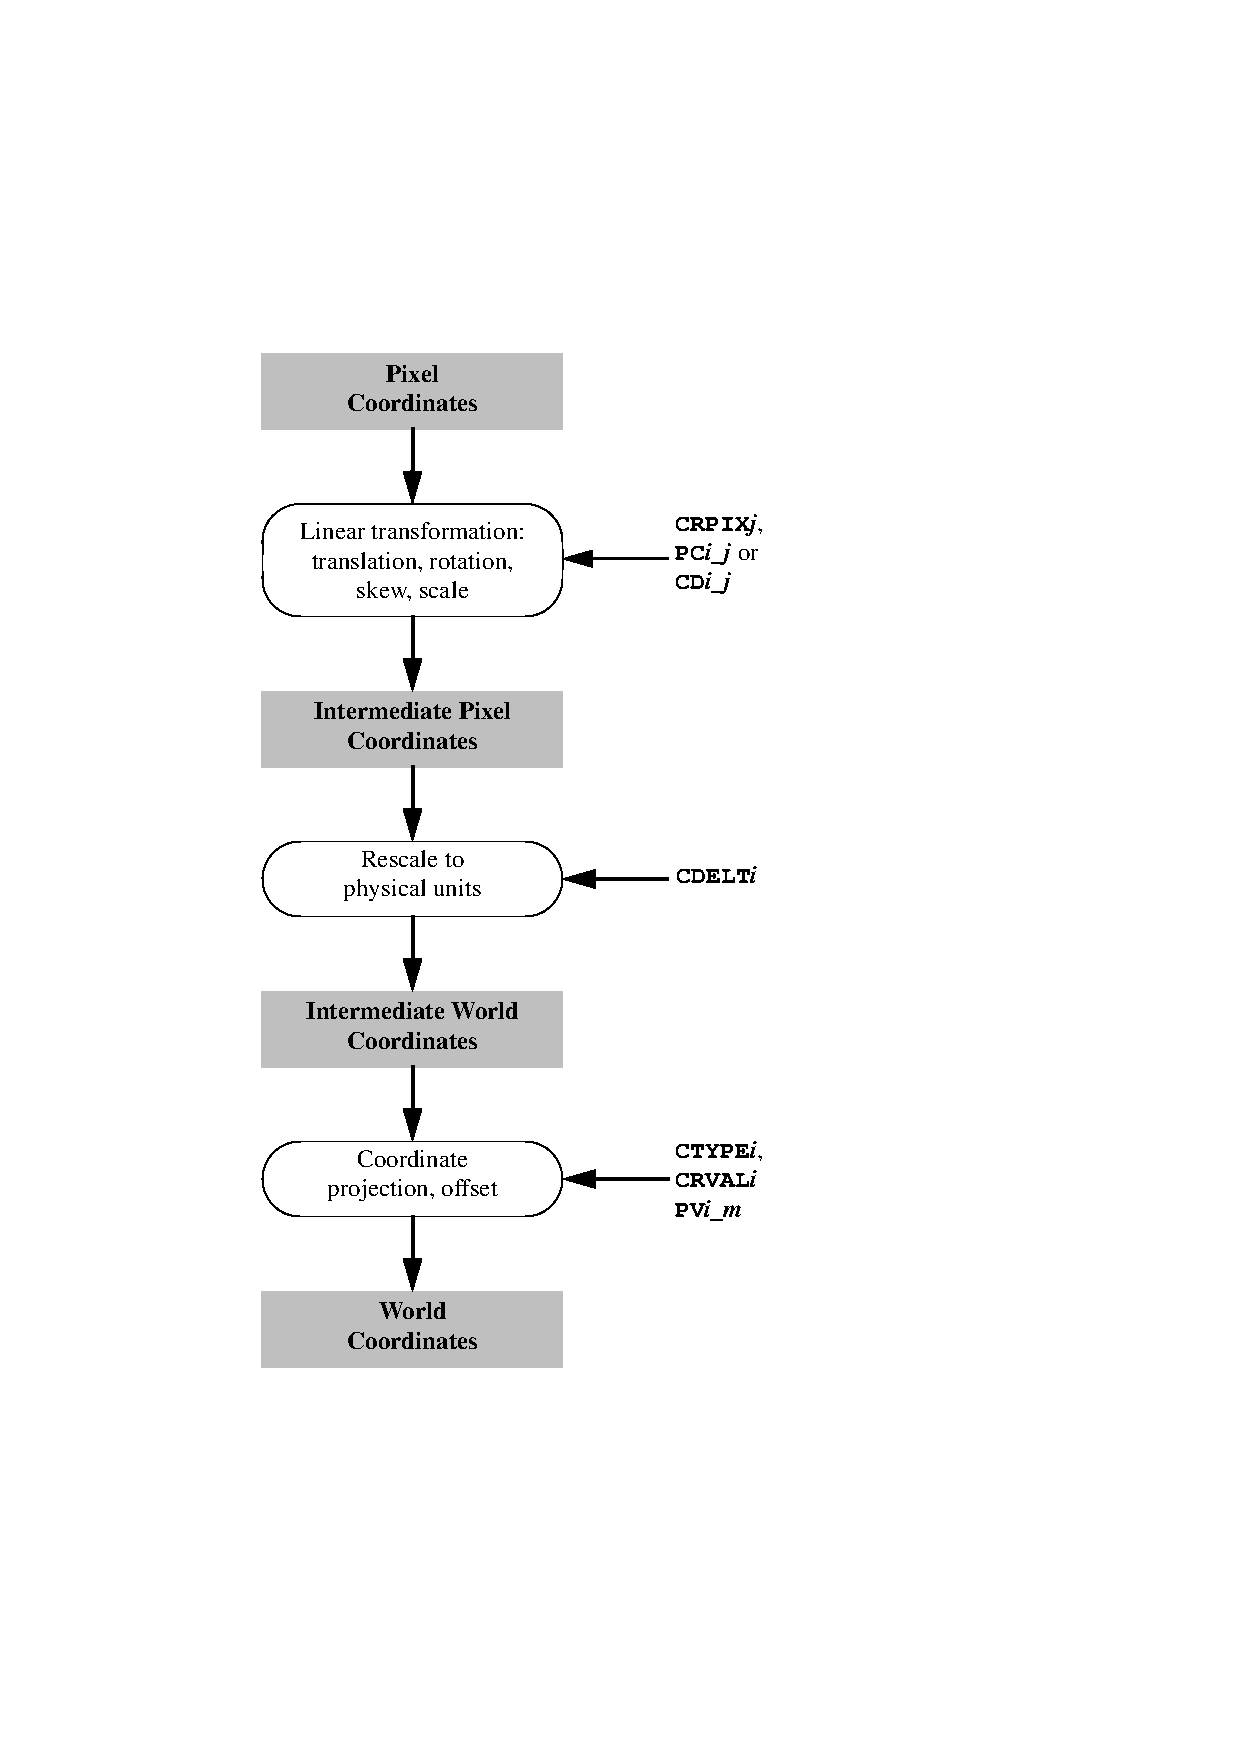
\includegraphics[scale=0.50]{WCSfig.pdf}
\leavevmode
\epsfysize=9.0cm
\epsffile{WCSfig.eps}
\caption{A schematic view of converting pixel coordinates to world coordinates.}
\label{fig:px2wld}
\end{center}
\end{figure}
%

For all coordinate types, the first step is a linear
transformation applied via matrix multiplication of the vector of 
pixel coordinate elements, $p_j$:  
\begin{equation}
q_i = \sum_{j=1}^{N} m_{ij} (p_j - r_j)  \label{eq:pix2intpix}
\end{equation}
where $r_j$ are the pixel coordinate
elements of the reference point, $j$ indexes the pixel axis, and $i$ the world
axis. The $m_{ij}$ matrix is a non-singular, square matrix of dimension 
$N\times N$, where $N$ is the number of world coordinate axes.  
%Often, $N$ is given by the \kwd{NAXIS} keyword, but this will be generalized with the discussion of the \kwd{WCSAXES} keyword, below.  
The elements $q_i$ of the resulting
\textit{intermediate pixel coordinate} vector are offsets, in dimensionless pixel
units, from the reference point along axes coincident with those of the
\textit{intermediate world coordinates}. Thus, the conversion of $q_i$ to the
corresponding intermediate world coordinate element $x_i$ is a simple scale:
\begin{equation} 
x_i = s_iq_i.  \label{eq:intpix2intworld} 
\end{equation}

There are three conventions for associating {\em FITS\/} keywords with the above
transformations.  
In the first formalism, the matrix
elements $m_{ij}$ are encoded in the \indxkw{PC}{i\_j} keywords and the scale
factors $s_i$ are encoded in the \indxkw{CDELT}{i} keywords, which {\em must}
have non-zero values. In the second formalism Eqs.~(\ref{eq:pix2intpix}) and
(\ref{eq:intpix2intworld}) are combined as  
\begin{equation}
x_i = \sum_{j=1}^{N} (s_i m_{ij}) (p_j - r_j)  \label{eq:pix2intworld}
\end{equation}
and the
\indxkw{CD}{i\_j} keywords encode the product $s_i m_{ij}$.   
The third convention was widely used before the development
of the 2 previously described conventions and
uses the \indxkw{CDELT}{i} keywords to define the image scale and the
{\tt CROTA2} keyword to define a bulk rotation of the image plane.  
Use of the {\tt CROTA2} keyword is now deprecated, \index{deprecate} 
and instead the newer
\indxkw{PC}{i\_j} or \indxkw{CD}{i\_j} keywords are {\em recommended} because they
allow for skewed axes and fully general rotation of multi-dimensional arrays. 
The
\indxkw{CDELT}{i} and {\tt CROTA2} keywords {\em may} co-exist with the
\indxkw{CD}{i\_j} keywords 
(but the {\tt CROTA2} {\em must not} occur with the \indxkw{PC}{i\_j} keywords)
as an aid to old {\em FITS\/}
interpreters, but these keywords  {\em must} be
ignored by software that supports the \indxkw{CD}{i\_j} keyword convention.
 In all these formalisms the reference pixel coordinates $r_j$ are encoded in
the \indxkw{CRPIX}{i} keywords, and the world coordinates at the reference point
are encoded in the \indxkw{CRVAL}{i} keywords. For additional details, see \cite{greisen02}. 

The third step of the process, computing the final world coordinates, depends on
the type of coordinate system, which is indicated with the value of the
\indxkw{CTYPE}{i} keyword. For some simple, linear cases an appropriate choice of
normalization for the scale factors allows the world coordinates to be taken
directly (or by applying a constant offset) from the $x_i$ (e.g., some spectra).
In other cases it is more complicated, and may require the application of some
non-linear algorithm (e.g., a projection, as for celestial coordinates), which may
require the specification of additional parameters. Where necessary, numeric
parameter values for non-linear algorithms {\em must} be specified via
\indxkw{PV}{i\_m} keywords and character-valued parameters will be specified via
\indxkw{PS}{i\_m} keywords, where $m$ is the parameter number. 

The application of these formalisms to coordinate systems of interest is discussed
in the following sub-sections: \S\ref{sect:WCSkw} describes general WCS
representations (see \cite{greisen02}), \S\ref{sect:Celestkw} describes celestial coordinate
systems (see \cite{calabretta02}), and \S\ref{sect:SPECkw} describes spectral coordinate systems
(see \cite{greisen06}). 

\section{World Coordinate System Representations}\label{sect:WCSkw}

A variety of keywords have been reserved for computing the coordinate values that
are to be associated with any pixel location within an array. The full set is
given in Table~\ref{ta:WCSkw}; those in most common usage are defined in detail below for
convenience. Coordinate system specifications may appear in HDUs that contain
simple images in the primary array or in an image extension.  Images may also be 
stored in a  multi-dimensional vector cell of a binary table, or as a tabulated list of
pixel locations (and optionally, the pixel value) in a table.  In these latter 2 types
of image representations, the WCS keywords have a different naming convention 
which reflects the needs of the tabular data structure
and the 8-character limit for keyword lengths, but otherwise follow exactly the
same rules for type, usage, and default values. See reference \cite{calabretta02}
for example usage of these keywords.
All forms of these reserved keywords
{\em must} be used only as specified in this Standard. 

%% Complete table of WCS keywords
%\clearpage
\begin{deluxetable}{llllll}
\tabletypesize{\scriptsize}
%\tabletypesize{\tiny}
\tablecolumns{6}
\tablewidth{0pt}
\renewcommand{\arraystretch}{.9}
\tablecaption{Reserved WCS Keywords 
\label{ta:WCSkw}}
\tablehead {
\colhead{Keyword} & \colhead{Primary} &\multicolumn{2}{c}{BINTABLE vector} & \multicolumn{2}{c}{Pixel List} \\
\cline{3-4} \cline{5-6}
%
\colhead{Description} & \colhead{Array} & \colhead{primary} & \colhead{alternative} & \colhead{primary} &
\colhead{alternative} 
}
%
\startdata
Coordinate dimensionality & \kwdalt{WCSAXES} & \multicolumn{2}{c}{\indxkwdalt{WCAX}{n}} & \multicolumn{2}{c}{\ldots} \\
Axis type			& \indxkwdalt{CTYPE}{i} & \dindxkw{i}{CTYP}{n} & \dindxkw{i}{CTY}{na} & \indxkw{TCTYP}{n} & \indxkwdalt{TCTY}{n} \\
%
 Axis units			& \indxkwdalt{CUNIT}{i} & \dindxkw{i}{CUNI}{n} & \dindxkw{i}{CUN}{na} & \indxkw{TCUNI}{n} & \indxkwdalt{TCUN}{n}\\
 Reference value	& \indxkwdalt{CRVAL}{i} & \dindxkw{i}{CRVL}{n} & \dindxkw{i}{CRV}{na} & \indxkw{TCRVL}{n} & \indxkwdalt{TCRV}{n} \\
 Coordinate increment  & \indxkwdalt{CDELT}{i} & \dindxkw{i}{CDLT}{n} & \dindxkw{i}{CDE}{na} & \indxkw{TCDLT}{n} & \indxkwdalt{TCDE}{n} \\
 Reference point       & \indxkwdalt{CRPIX}{j} & \dindxkw{j}{CRPX}{n} & \dindxkw{j}{CRP}{na} & \indxkw{TCRPX}{n} & \indxkwdalt{TCRP}{n} \\
 Coordinate rotation\tablenotemark{1} & \indxkw{CROTA}{i} & \dindxkw{i}{CROT}{n} &  & \indxkw{TCROT}{n} & \\
 Transformation matrix\tablenotemark{2} & \indxkwdalt{PC}{i\_j} & \multicolumn{2}{c}{\dindxkwalt{ij}{PC}{n}} & \multicolumn{2}{c}{\indxkwdalt{TPC}{n\_k} or \indxkwdalt{TP}{n\_k}} \\
 Transformation matrix\tablenotemark{2} & \indxkwdalt{CD}{i\_j} & \multicolumn{2}{c}{\dindxkwalt{ij}{CD}{n}} & \multicolumn{2}{c}{\indxkwdalt{TCD}{n\_k} or \indxkwdalt{TC}{n\_k}} \\

 Coordinate parameter & \indxkwdalt{PV}{i\_m} & \multicolumn{2}{c}{\dindxkwalt{i}{PV}{n\_m} or \dindxkwalt{i}{V}{n\_m}} & \multicolumn{2}{c}{\indxkwdalt{TPV}{n\_m} or \indxkwdalt{TV}{n\_m}} \\
 Coordinate parameter array &  \nodata  & \multicolumn{2}{c}{\dindxkw{i}{V}{n}\kwdalt{\_X}} & \multicolumn{2}{c}{\nodata} \\
 Coordinate parameter  & \indxkwdalt{PS}{i\_m} & \multicolumn{2}{c}{\dindxkwalt{i}{PS}{n\_m} or \dindxkwalt{i}{S}{n\_m}} & \multicolumn{2}{c}{\indxkwdalt{TPS}{n\_m} or \indxkwdalt{TS}{n\_m}} \\
 Coordinate name	& \kwdalt{WCSNAME} & \multicolumn{2}{c}{\indxkwdalt{WCSN}{n}} & \multicolumn{2}{c}{\indxkwdalt{WCS}{n} or \indxkwdalt{TWCS}{n}} \\
 Coordinate axis name & \indxkwdalt{CNAME}{i} & \multicolumn{2}{c}{\dindxkwalt{i}{CNA}{n}} & \multicolumn{2}{c}{\indxkwdalt{TCNA}{n}} \\

 Random error		& \indxkwdalt{CRDER}{i} & \multicolumn{2}{c}{\dindxkwalt{i}{CRD}{n}} & \multicolumn{2}{c}{\indxkwdalt{TCRD}{n}} \\
 Systematic error	& \indxkwdalt{CSYER}{i} & \multicolumn{2}{c}{\dindxkwalt{i}{CSY}{n}} & \multicolumn{2}{c}{\indxkwdalt{TCSY}{n}} \\
 WCS cross-ref.~target & \nodata  & \multicolumn{2}{c}{\indxkwdalt{WCST}{n}} & \multicolumn{2}{c}{\nodata} \\
 WCS cross reference   & \nodata  & \multicolumn{2}{c}{\indxkwdalt{WCSX}{n}} & \multicolumn{2}{c}{\nodata} \\
 Coordinate rotation & \kwdalt{LONPOLE} & \multicolumn{2}{c}{\indxkwdalt{LONP}{n}} & \multicolumn{2}{c}{\indxkwdalt{LONP}{n}} \\
 Coordinate rotation & \kwdalt{LATPOLE} & \multicolumn{2}{c}{\indxkwdalt{LATP}{n}} & \multicolumn{2}{c}{\indxkwdalt{LATP}{n}} \\
 Coordinate epoch	& \kwdalt{EQUINOX} & \multicolumn{2}{c}{\indxkwdalt{EQUI}{n}} & \multicolumn{2}{c}{\indxkwdalt{EQUI}{n}} \\
 Coordinate epoch\tablenotemark{3}	& \kwd{EPOCH} & \multicolumn{2}{c}{\kwd{EPOCH}} & \multicolumn{2}{c}{\kwd{EPOCH}} \\
Date of observation & \kwd{MJD-OBS} & \multicolumn{2}{c}{\indxkw{MJDOB}{n}} & \multicolumn{2}{c}{\indxkw{MJDOB}{n}} \\
 Average date of obs & \kwd{MJD-AVG} & \multicolumn{2}{c}{\indxkw{MJDA}{n}} & \multicolumn{2}{c}{\indxkw{MJDA}{n}} \\
 Date/time of observation & \kwd{DATE-OBS} & \multicolumn{2}{c}{\indxkw{DOBS}{n}} & \multicolumn{2}{c}{\indxkw{DOBS}{n}} \\
 Average date/time of obs & \kwd{DATE-AVG} & \multicolumn{2}{c}{\indxkw{DAVG}{n}} & \multicolumn{2}{c}{\indxkw{DAVG}{n}} \\

 Reference frame	& \kwdalt{RADESYS} or & \multicolumn{2}{c}{\indxkwdalt{RADE}{n}} & \multicolumn{2}{c}{\indxkwdalt{RADE}{n}} \\
  	&  {\tt RADECSYS}\tablenotemark{4} & \multicolumn{2}{c}{ } & \multicolumn{2}{c}{ } \\

 Line rest frequency (Hz) & \kwdalt{RESTFRQ} or  & \multicolumn{2}{c}{\indxkwdalt{RFRQ}{n}} & \multicolumn{2}{c}{\indxkwdalt{RFRQ}{n}} \\
        & \kwd{RESTFREQ}\tablenotemark{4} & \multicolumn{2}{c}{\nodata} & \multicolumn{2}{c}{\nodata} \\
 Line rest vac wavelength (m) & \kwdalt{RESTWAV} & \multicolumn{2}{c}{\indxkwdalt{RWAV}{n}} & \multicolumn{2}{c}{\indxkwdalt{RWAV}{n}} \\
 Spectral reference frame & \kwdalt{SPECSYS} & \multicolumn{2}{c}{\indxkwdalt{SPEC}{n}} & \multicolumn{2}{c}{\indxkwdalt{SPEC}{n}} \\
 Spectral reference frame & \kwdalt{SSYSOBS} & \multicolumn{2}{c}{\indxkwdalt{SOBS}{n}} & \multicolumn{2}{c}{\indxkwdalt{SOBS}{n}} \\
 Spectral reference frame & \kwdalt{SSYSSRC} & \multicolumn{2}{c}{\indxkwdalt{SSRC}{n}} & \multicolumn{2}{c}{\indxkwdalt{SSRC}{n}} \\
 Observation X (m)	& \kwd{OBSGEO-X} & \multicolumn{2}{c}{\indxkw{OBSGX}{n}} & \multicolumn{2}{c}{\indxkw{OBSGX}{n}} \\
 Observation Y (m)	& \kwd{OBSGEO-Y} & \multicolumn{2}{c}{\indxkw{OBSGY}{n}} & \multicolumn{2}{c}{\indxkw{OBSGY}{n}} \\
 Observation Z (m)	& \kwd{OBSGEO-Z} & \multicolumn{2}{c}{\indxkw{OBSGZ}{n}} & \multicolumn{2}{c}{\indxkw{OBSGZ}{n}} \\
 Radial velocity (m s$^{-1}$) & \kwdalt{VELOSYS} & \multicolumn{2}{c}{\indxkwdalt{VSYS}{n}} & \multicolumn{2}{c}{\indxkwdalt{VSYS}{n}} \\
 Redshift of source & \kwdalt{ZSOURCE} & \multicolumn{2}{c}{\indxkwdalt{ZSOU}{n}} & \multicolumn{2}{c}{\indxkwdalt{ZSOU}{n}} \\
 Angle of true velocity & \kwdalt{VELANGL} & \multicolumn{2}{c}{\indxkwdalt{VANG}{n}} & \multicolumn{2}{c}{\indxkwdalt{VANG}{n}} \\

\enddata
\tablenotetext{1}{\indxkw{CROTA}{i} form is deprecated but still in use.
It {\em must not} be used with \PCij, \PV{i}{m}, and \PS{i}{m}.}
\tablenotetext{2}{\indxkw{PC}{i\_j} and \indxkw{CD}{i\_j} forms of the transformation 
matrix are mutually exclusive, and {\em must not} appear together in the same HDU.}
\tablenotetext{3}{\kwd{EPOCH} is deprecated. Use \kwd{EQUINOX} instead.}
\tablenotetext{4}{These 8-character keywords are deprecated; the 7-character forms, which can include an alternate version code letter 
at the end, {\em should} be used instead.}
%
\tablecomments{The indexes {\it j} and {\it i} are pixel and intermediate world coordinate axis numbers, respectively. 
Within a table, the index {\it n} refers to a column number, and {\it m} refers to a coordinate parameter number. 
The index {\it k} also refers to a column number.
The indicator {\it a} is either blank (for the primary coordinate description) or a character {\tt A} through {\tt Z} 
that specifies the coordinate version. See text.}
%
\end{deluxetable}


The keywords given below constitute a complete set of fundamental attributes for a
WCS description. Although their inclusion in an HDU is optional, {\em FITS\/} writers
{\em should} include a complete set of keywords when describing a WCS. In the
event that some keywords are missing, default values {\em must} be assumed, as
specified below. 

\begin{description}

\item \kwd{WCSAXES} --- [integer; default: \kwd{NAXIS}, or 
largest of WCS indexes $i$ or $j$]\\ 
Number of axes in the WCS description. This keyword, if present,
{\em must} precede all WCS keywords except \kwd{NAXIS} in the HDU. The value of
\kwd{WCSAXES} {\em may} exceed the number of pixel axes for the HDU. 

\item \indxkw{CTYPE}{i} --- [character; indexed; default: \texttt{`\ '} (i.e.\ a
linear, undefined axis)] \\ 
Type for the intermediate coordinate axis $i$. Any
coordinate type that is not covered by this standard or an officially recognized
{\em FITS\/} convention {\em shall} be taken to be linear. All non-linear coordinate
system names {\em must} be expressed in ``4--3" form: the first four characters
specify the coordinate type, the fifth character is a hyphen (`{\tt -}'), and the
remaining three characters specify an algorithm code for computing the world
coordinate value. Coordinate types with names of less than four characters are
padded on the right with hyphens, and algorithm codes with less than three
characters are padded on the right with blanks\footnote[1]{Example: 
\texttt{`RA---UV~'}.}. 
Algorithm codes {\em should} be three characters. 

\item \indxkw{CUNIT}{i} --- [character; indexed; default: \texttt{`\ '} (i.e.,
undefined)]\\ 
Physical units of \kwd{CRVAL} and \kwd{CDELT} for axis {\it i}. Note
that units {\em should} always be specified (see \S\ref{s:Units}). Units for celestial
coordinate systems defined in this Standard {\em must} be degrees. 

\item \indxkw{CRPIX}{j} --- [floating-point; indexed; default: 0.0]\\ 
Location of the reference point in the image for axis $j$
corresponding to $r_j$ in Eq.~(\ref{eq:pix2intpix}).  Note that the
reference point {\em may} lie outside the image and that the first pixel
in the image has pixel coordinates $(1.0, 1.0, \ldots)$. 

\item \indxkw{CRVAL}{i} --- [floating-point; indexed; default: 0.0]\\ 
World Coordinate value at the reference point of axis $i$.

\item \indxkw{CDELT}{i} --- [floating-point; indexed; default: 1.0]\\ 
Increment of the world coordinate at the reference point for axis $i$. 
The value {\em must not} be zero.

\item \indxkw{CROTA}{i} --- [floating-point; indexed; default: 0.0]\\
The amount of rotation from the standard coordinate
system to a different coordinate system.  Further use of this of this keyword
is deprecated, \index{deprecate} in favor of the newer formalisms that use the
\indxkw{CD}{i\_j} or \indxkw{PC}{i\_j} keywords to define the rotation.

\item \indxkw{PC}{i\_j}  --- [floating-point; defaults: 1.0 when $i=j$, 0.0
otherwise]\\ 
Linear transformation matrix between pixel axes $j$ and intermediate
coordinate axes $i$. The \indxkw{PC}{i\_j} matrix {\em must not} be singular. 

\item \indxkw{CD}{i\_j}  --- [floating-point; defaults: 0.0, but see below]\\
Linear transformation matrix (with scale) between pixel axes $j$ and intermediate
coordinate axes $i$. This nomenclature is equivalent to \indxkw{PC}{i\_j} when
\indxkw{CDELT}{i} is unity. The \indxkw{CD}{i\_j} matrix {\em must not} be
singular. Note that the \indxkw{CD}{i\_j} formalism is an exclusive alternative to
\indxkw{PC}{i\_j}, and the \indxkw{CD}{i\_j} and \indxkw{PC}{i\_j}  keywords
{\em must not} appear together within an HDU. 

\end{description}

\noindent In addition to the restrictions noted above, if any \indxkw{CD}{i\_j}
keywords are present in the HDU, all other unspecified \indxkw{CD}{i\_j} keywords
{\em shall} default to zero. If no \indxkw{CD}{i\_j} keywords are present then
the header {\em shall} be interpreted as being in \indxkw{PC}{i\_j} form whether
or not any \indxkw{PC}{i\_j} keywords are actually present in the HDU.  

Some non-linear algorithms that describe the transformation between pixel and
intermediate coordinate axes require parameter values. A few non-linear algorithms
also require character-valued parameters, e.g., table lookups require the names of
the table extension and the columns to be used. Where necessary parameter values
{\em must} be specified via the following keywords: 

\begin{description}

\item \indxkw{PV}{i\_m}  --- [floating-point]\\ 
Numeric parameter values for
intermediate world coordinate axis $i$, where $m$ is the parameter number. Leading
zeros {\em must not} be used, and $m$ may have only values in the range 0 through 99,
and that are defined for the particular non-linear algorithm. 

\item \indxkw{PS}{i\_m}  --- [character]\\ 
Character-valued parameters for
intermediate world coordinate axis $i$, where $m$ is the parameter number. Leading
zeros {\em must not} be used, and $m$ may have only values in the range 0 through 99,
and that are defined for the particular non-linear algorithm. 

\end{description}

The following keywords, while not essential for a complete specification of an
image WCS, can be extremely useful for readers to interpret the accuracy of the
WCS representation of the image. 

\begin{description}

\item \indxkw{CRDER}{i}  --- [floating-point; default: 0.0]\\ 
Random error in coordinate $i$, which {\em must} be non-negative. 

\item \indxkw{CSYER}{i}  --- [floating-point; default: 0.0]\\ 
Systematic error in coordinate $i$, which {\em must} be non-negative. 

\end{description}

\noindent These values {\em should} give a representative average value of the
error over the range of the coordinate in the HDU. The total error in the
coordinates would be given by summing the individual errors in quadrature. 

\subsection{Alternative WCS Axis Descriptions}

In some cases it is useful to describe an image with more than one coordinate 
type\footnote[1]{Examples include the frequency, velocity, and wavelength along a
spectral axis (only one of which, of course, could be linear), or the position
along an imaging detector in both meters and degrees on the sky.}.  Alternative WCS
descriptions {\em may} be added to the header by adding the appropriate sets of
WCS keywords, and appending to all keywords in each set an alphabetic code in the
range {\tt A} through {\tt Z}. Keywords that may be used in this way to specify a
coordinate system version are indicated in Table~\ref{ta:WCSkw} with the suffix \textit{a}.
All implied keywords with this encoding are {\em reserved keywords}, and
{\em must} only be used in {\em FITS\/} HDUs as specified in this Standard. The axis
numbers {\em must} lie in the range 1 through 99, and the coordinate parameter $m$
{\em must} lie in the range 0 through 99, both with no leading zeros. 

The {\em primary} version of the WCS description is that specified with {\it a}
as the blank character\footnote[2]{There are a number of keywords  (e.g. \dindxkwalt{ij}{PC}{n})
where the {\it a} could be pushed off the 8-char keyword name for plausible
values of {\it i}, {\it j}, {\it k}, {\it n}, and {\it m}.  
In such cases {\it a} is still said to be ``blank''
although it is not the blank character.}.
Alternative axis descriptions are optional, but {\em must
not} be specified unless the primary WCS description is also specified. If an
alternative WCS description is specified, all coordinate keywords for that version
{\em must} be given even if the values do not differ from those of the primary
version. Rules for the default values of alternative coordinate descriptions are the
same as those for the primary description. The alternative descriptions are computed
in the same fashion as the primary coordinates. The type of coordinate depends on
the value of \indxkwdalt{CTYPE}{i}, and may be linear in one of the alternative
descriptions and non-linear in another. 

The alternative version codes are selected by the {\em FITS\/} writer; there is no
requirement that the codes be used in alphabetic sequence, nor that one coordinate
version differ in its parameter values from another. An optional keyword
\kwdalt{WCSNAME} is also defined to name, and otherwise document, the various
versions of WCS descriptions: 

\begin{description}

\item \kwdalt{WCSNAME}  --- [character; default for {\bf a}: \texttt{`\ '} (i.e.,
blank, for the primary WCS, else a character {\tt A} through {\tt Z} that
specifies the coordinate version]\\ 
Name of the world coordinate system represented by
the WCS keywords with the suffix {\bf a}. Its primary function is to provide a
means by which to specify a particular WCS if multiple versions are defined in the
HDU. 

\end{description}

\section{Celestial Coordinate System Representations}\label{sect:Celestkw}

The conversion from intermediate world coordinates $(x,y)$ in the plane of
projection to celestial coordinates involves two steps: a spherical projection to
native longitude and latitude $(\phi, \theta)$, defined in terms of a convenient
coordinate system (i.e., \textit{native spherical coordinates}), followed by a
spherical rotation of these native coordinates to the required celestial
coordinate system $(\alpha, \delta)$. The algorithm to be used to define the
spherical projection {\em must} be encoded in the \indxkw{CTYPE}{i} keyword as
the three-letter algorithm code, the allowed values for which are specified in
Table~\ref{ta:PROJcode} and defined in references \cite{calabretta02} and 
\cite{calabretta07}.
The target celestial coordinate system is also encoded into the
left-most portion of the \indxkw{CTYPE}{i} keyword as the coordinate type.

%%% Celestial Coordinate projection algorithm codes
%\clearpage
\begin{deluxetable}{lllll}
\tabletypesize{\small}
%\tabletypesize{\scriptsize}
\tablecolumns{5}
\tablewidth{0pt}
\tablecaption{Reserved Celestial Coordinate Algorithm Codes 
\label{ta:PROJcode}}
\tablehead {
\colhead{} & \multicolumn{2}{c}{Default} & \colhead{ } & \colhead{ } \\
\cline{2-3}
\colhead{Code} & \colhead{$\phi_0$} & \colhead{$\theta_0$} & \colhead{Properties\tablenotemark{1}} & \colhead{Projection Name}
}
%
\startdata
%
%\cutinhead{Zenithal (azimuthal) projections}
\multicolumn{5}{c}{Zenithal (azimuthal) projections} \\
\kwd{AZP} & 0\degr & 90\degr & \S5.1.1 & Zenithal perspective \\
\kwd{SZP} & 0\degr & 90\degr & \S5.1.2 & Slant zenithal perspective \\
\kwd{TAN} & 0\degr & 90\degr & \S5.1.3 & Gnomonic \\
\kwd{STG} & 0\degr & 90\degr & \S5.1.4 & Stereographic \\
\kwd{SIN} & 0\degr & 90\degr & \S5.1.5 & Slant orthographic \\
\kwd{ARC} & 0\degr & 90\degr & \S5.1.6 & Zenithal equidistant \\
\kwd{ZPN} & 0\degr & 90\degr & \S5.1.7 & Zenithal polynomial \\
\kwd{ZEA} & 0\degr & 90\degr & \S5.1.8 & Zenithal equal-area \\
\kwd{AIR} & 0\degr & 90\degr & \S5.1.9 & Airy \\
\hline 
%
%\cutinhead{Cylindrical projections}
\multicolumn{5}{c}{Cylindrical projections} \\
\kwd{CYP} & 0\degr & 0\degr & \S5.2.1. & Cylindrical perspective \\
\kwd{CEA} & 0\degr & 0\degr & \S5.2.2 & Cylindrical equal area \\
\kwd{CAR} & 0\degr & 0\degr & \S5.2.3 & Plate carr\'ee \\
\kwd{MER} & 0\degr & 0\degr & \S5.2.4 & Mercator \\
\hline 
%
\multicolumn{5}{c}{Pseudo-cylindrical and related projections} \\
\kwd{SFL} & 0\degr & 0\degr & \S5.3.1 & Samson-Flamsteed \\
\kwd{PAR} & 0\degr & 0\degr & \S5.3.2 & Parabolic \\
\kwd{MOL} & 0\degr & 0\degr & \S5.3.3 & Mollweide\\
\kwd{AIT} & 0\degr & 0\degr & \S5.3.4 & Hammer-Aitoff \\
\hline 
%
\multicolumn{5}{c}{Conic projections} \\
\kwd{COP} & 0\degr & $\theta_a$ & \S5.4.1 & Conic perspective \\
\kwd{COE} & 0\degr & $\theta_a$& \S5.4.2 & Conic equal-area \\
\kwd{COD} & 0\degr & $\theta_a$& \S5.4.3 & Conic equidistant \\
\kwd{COO} & 0\degr & $\theta_a$ & \S5.4.4 & Conic orthomorphic \\
\hline 
%
\multicolumn{5}{c}{Polyconic and pseudoconic projections} \\
\kwd{BON} & 0\degr & 0\degr & \S5.5.1 & Bonne's equal area \\
\kwd{PCO} & 0\degr & 0\degr & \S5.5.2 & Polyconic \\
\hline 
%
\multicolumn{5}{c}{Quad-cube projections} \\
\kwd{TSC} & 0\degr & 0\degr & \S5.6.1 & Tangential spherical cube \\
\kwd{CSC} & 0\degr & 0\degr & \S5.6.2 & COBE quadrilateralized spherical cube \\
\kwd{QSC} & 0\degr & 0\degr & \S5.6.3 & Quadrilateralized spherical cube \\
\hline 
%
\multicolumn{5}{c}{HEALPix grid projection} \\
\kwd{HPX} & 0\degr & 0\degr & \S6\tablenotemark{2} & HEALPix grid \\
%
\enddata
\tablenotetext{1}{Refer to the indicated section in reference \cite{calabretta02} for a detailed description.}
\tablenotetext{2}{This projection is defined in reference \cite{calabretta07}. }
\end{deluxetable}

For the final step, the parameter \kwdalt{LONPOLE} must be specified, which is the
native longitude of the celestial pole, $\phi_p$. For certain projections (such as
cylindricals and conics, which are less commonly used in astronomy), the
additional keyword \kwdalt{LATPOLE} must be used to specify the native latitude of
the celestial pole. See \cite{calabretta02} for the transformation equations and other details. 

The accepted celestial coordinate systems are: the standard equatorial
(\texttt{RA--} and \texttt{DEC-}), and others of the form $x${\tt LON} and $x${\tt
LAT} for longitude-latitude pairs, where $x$ is {\tt G} for Galactic, {\tt E} for
ecliptic, {\tt H} for helioecliptic and {\tt S} for supergalactic coordinates.
Since the representation of planetary, lunar, and solar coordinate systems could
exceed the 26 possibilities afforded by the single character $x$, pairs of the
form $yz${\tt LN} and $yz${\tt LT} {\em may} be used as well. 

\begin{description}

\item \kwdalt{RADESYS}  --- [character; default: \texttt{FK4}, \texttt{FK5}, or
\texttt{ICRS}: see below]\\ 
Name of the reference frame of equatorial or ecliptic
coordinates, whose value {\em must} be one of those specified in Table~\ref{ta:RADESYS}. The
default value is \texttt{FK4} if the value of \kwdalt{EQUINOX} $<1984.0$,
\texttt{FK5} if \kwdalt{EQUINOX} $\geq1984.0$, or \texttt{ICRS} if
\kwdalt{EQUINOX} is not given.


\item \kwdalt{EQUINOX}  --- [floating-point; default: see below]\\ 
Epoch of the mean
equator and equinox in years, whose value {\em must} be non-negative. The
interpretation of epoch depends upon the value of \kwdalt{RADESYS} if present:
{\em Besselian} if the value is \texttt{FK4} or \texttt{FK4-NO-E}, {\em Julian}
if the value is \texttt{FK5}; {\em not applicable} if the value is \texttt{ICRS}
or \texttt{GAPPT}. 

\item \kwd{EPOCH}  --- [floating-point]\\ 
  This keyword is deprecated \index{deprecate} and {\em should not} be used in new 
  {\em FITS\/} files.  It is reserved primarily to prevent its use
  with other meanings.  The {\tt EQUINOX} keyword\index{EQUINOX} 
  {\em shall} be used instead.  The value field of this
  keyword was previously defined to contain a floating-point number\index{EPOCH}
 giving the equinox in years for the celestial 
 coordinate system\index{coordinate system}
 in which positions are expressed.


\item \kwd{DATE-OBS}  --- [floating-point]\\
This reserved keyword is defined in \S\ref{s:kobs}. 

\item \kwd{MJD-OBS}  --- [floating-point; default: \kwd{DATE-OBS} if given,
otherwise no default]\\ 
Modified Julian Date (JD -- 2,400,000.5) of the
observation, whose value corresponds (by default) to the {\em start} of the
observation, unless another interpretation is explained in the comment field. 
No specific time system (e.g. UTC, TAI, etc.) is defined for this or any of
the other time-related keywords.  It is {\em recommended} that 
the \kwd{TIMESYS} keyword, as defined in Appendix B be used to specify the
time system.

\item \kwdalt{LONPOLE}  --- [floating-point; default: $\phi_0$ if $\delta_0 \geq
\theta_0$,  $\phi_0+180\degr$ otherwise]\\ 
Longitude in the native coordinate
system of the celestial system's north pole. Normally, $\phi_0$ is zero unless a
non-zero value has been set for {\tt PV}{\it i}{\tt \_1}{\bf a}, which is
associated with the {\em longitude} axis. This default applies for all values of
$\theta_0$, including $\theta_0=90\degr$, although the use of non-zero values of
$\theta_0$ are discouraged in that case. 

\item \kwdalt{LATPOLE}  --- [floating-point; default: 90\degr, or no default if
$(\theta_0,\delta_0,\phi_p-\phi_0) = (0,0,\pm90\degr)$]\\ 
Latitude in the native
coordinate system of the celestial system's north pole, or equivalently, the
latitude in the celestial coordinate system of the native system's north pole. May
be ignored or omitted in cases where \kwdalt{LONPOLE} completely specifies the
rotation to the target celestial system. 

\end{description}

%\clearpage
\begin{deluxetable}{ll}
%\tabletypesize{\footnotesize}
%\tabletypesize{\scriptsize}
%\tabletypesize{\tiny}
\tablecolumns{2}
\tablewidth{0pt}
\tablecaption{Allowed Values of \kwdalt{RADESYS} 
\label{ta:RADESYS}}
\tablehead {
\colhead{Value} & \colhead{Definition}  
}
%
\startdata
\kwd{ICRS} & International Celestial Reference System \\
\kwd{FK5} & Mean place, new (IAU 1984) system \\
\kwd{FK4}\tablenotemark{1} & Mean place, old (Bessel-Newcomb) system \\
\kwd{FK4-NO-E}\tablenotemark{1} & Mean place:  but without eccentricity terms \\ 
\kwd{GAPPT} & Geocentric apparent place, IAU 1984 system \\
%
\enddata
\tablenotetext{1}{New FITS files should avoid using these older reference systems.}
\end{deluxetable}

\section{Spectral Coordinate System Representations}\label{sect:SPECkw}

This section discusses the conversion of intermediate world coordinates to
spectral coordinates with common axes such as frequency, wavelength, and apparent
radial velocity (represented here with the coordinate variables $\nu, \lambda$, or
$v$). The key point for constructing spectral WCS in {\em FITS\/} is that one of these
coordinates {\em must} be sampled linearly in the dispersion axis; the others are
derived from prescribed, usually non-linear transformations. Frequency and
wavelength axes {\em may} also be sampled linearly in their logarithm. 

Following the convention for the \indxkwdalt{CTYPE}{i} keyword, when $i$ is the
spectral axis the first four characters {\em must} specify a code for the
coordinate type; for non-linear algorithms the fifth character {\em must} be a
hyphen, and the next three characters {\em must} specify a predefined algorithm
for computing the world coordinates from the intermediate physical coordinates.
The coordinate type {\em must} be one of those specified in Table~\ref{ta:SPECtype}. When the
algorithm is linear, the remainder of the \indxkwdalt{CTYPE}{i} keyword
{\em must} be blank. When the algorithm is non-linear, the 3-letter algorithm
code {\em must} be one of those specified in Table~\ref{ta:SPECcode}. The relationships
between the basic physical quantities $\nu, \lambda$, and $v$, as well as the
relationships between various derived quantities are given in reference \cite{greisen06}. 

%%% Spectral Coordinate type codes
%\clearpage
\begin{deluxetable}{lllll}
%\tabletypesize{\footnotesize}
%\tabletypesize{\scriptsize}
\tablecolumns{5}
\tablewidth{0pt}
\tablecaption{Reserved Spectral Coordinate Type Codes\tablenotemark{1} 
\label{ta:SPECtype}}
\tablehead {
\colhead{Code} & \colhead{Type} & \colhead{Symbol} & \colhead{Assoc. Variable} & \colhead{Default Units}
}
%
\startdata
%
%\cutinhead{Zenithal (azimuthal) projections}
\kwd{FREQ} & Frequency & $\nu$ & $\nu$ & Hz \\
\kwd{ENER} & Energy 	& $E$ & $\nu$ & J \\
\kwd{WAVN} & Wavenumber & $\kappa$ & $\nu$ & m$^{-1}$ \\
\kwd{VRAD} & Radio velocity\tablenotemark{2} & $V$ & $\nu$ & m~s$^{-1}$ \\
\kwd{WAVE} & Vacuum wavelength & $\lambda$ & $\lambda$ & m \\
\kwd{VOPT} & Optical velocity\tablenotemark{2} & $Z$ & $\lambda$ & m~s$^{-1}$ \\
\kwd{ZOPT} & Redshift 	& $z$ & $\lambda$ & \nodata \\
\kwd{AWAV} & Air wavelength & $\lambda_a$ & $\lambda_a$ & m \\
\kwd{VELO} & Apparent radial velocity & $v$ & $v$ & m~s$^{-1}$ \\
\kwd{BETA} & Beta factor ($v/c$) & $\beta$ & $v$ & \nodata \\
%
\enddata
\tablenotetext{1}{Characters 1 through 4 of the value of the keyword \indxkwdalt{CTYPE}{i}.}
\tablenotetext{2}{By convention, the ``radio" velocity is given by $c(\nu_0 - \nu)/\nu_0$
and the ``optical" velocity is given by $c(\lambda - \lambda_0)/\lambda_0$.}
\end{deluxetable}

%%% Non-linear spectrum algorithm codes
%\clearpage
\begin{deluxetable}{lll}
%\tabletypesize{\footnotesize}
%\tabletypesize{\scriptsize}
\tablecolumns{3}
\tablewidth{0pt}
\tablecaption{Non-linear Spectral Algorithm Codes\tablenotemark{1}
\label{ta:SPECcode}}
\tablehead {
%\colhead{} & \multicolumn{2}{c}{Default} & \colhead{ } & \colhead{ } \\
%\cline{2-3}
\colhead{Code} & \colhead{Regularly sampled in} & \colhead{Expressed as}
}
%
\startdata
%
\kwd{F2W} & Frequency & Wavelength \\
\kwd{F2V} & & Apparent radial velocity \\
\kwd{F2A} & & Air wavelength \\

\kwd{W2F} & Wavelength & Frequency \\
\kwd{W2V} & & Apparent radial velocity \\
\kwd{W2A} & & Air wavelength \\

\kwd{V2F} & Apparent radial velocity & Frequency \\
\kwd{V2W} & & Wavelength \\
\kwd{V2A} & & Air wavelength \\

\kwd{A2F} & Air wavelength & Frequency \\
\kwd{A2W} & & Wavelength \\
\kwd{A2V} & & Apparent radial velocity \\
%
\cline{1-3}
\kwd{LOG} & Logarithm & Any 4-letter coordinate type \\
\kwd{GRI} & Detector & Any from Table~\ref{ta:SPECtype} \\
\kwd{GRA} & Detector & Any from Table~\ref{ta:SPECtype} \\
\kwd{TAB} & Not regular & Any 4-letter coordinate type \\
%
\enddata
\tablenotetext{1}{Characters 6 through 8 of the value of the keyword \indxkwdalt{CTYPE}{i}.}
\end{deluxetable}


The generality of the algorithm for specifying the spectral coordinate system and
its representation suggests that some additional description of the coordinate may
be helpful beyond what can be encoded in the first four characters of the
\indxkwdalt{CTYPE}{i} keyword; \indxkwdalt{CNAME}{i} is reserved for this purpose.
Note that this keyword provides a name for an axis in a particular WCS, while the
\kwdalt{WCSNAME} keyword names the particular WCS as a whole. In order to convert
between some form of radial velocity and either frequency or wavelength, the
keywords \kwdalt{RESTFRQ} and \kwdalt{RESTWAV}, respectively, are reserved. 

\begin{description}

\item \indxkwdalt{CNAME}{i}  --- [character; default: default: \texttt{`\ '}
(i.e.\ a linear, undefined axis)]\\ 
Spectral coordinate description which
{\em must not} exceed 68 characters in length. 

\item \kwdalt{RESTFRQ}  --- [floating-point; default: none]\\ 
Rest frequency of
the of the spectral feature of interest. The physical unit {\em must} be Hz.

\item \kwdalt{RESTWAV}  --- [floating-point; default: none]\\ 
Vacuum rest
wavelength of the of the spectral feature of interest. The physical unit
{\em must} be m.

\end{description}

\noindent One or the other of \kwdalt{RESTFRQ} or \kwdalt{RESTWAV} {\em should}
be given when it is meaningful to do so. 

\subsection{Spectral Coordinate Reference Frames}

Frequencies, wavelengths, and apparent radial velocities are always referred to
some selected standard of rest (i.e., reference frame). While the spectra are
obtained they are, of necessity, in the observer's rest frame. The velocity
correction from topocentric (the frame in which the measurements are usually made)
to standard reference frames (which {\em must} be one of those given in
Table~\ref{ta:SPECsys}) are dependent on the dot product with time-variable velocity vectors.
That is, the velocity with respect to a standard reference frame depends upon
direction, and the velocity (and frequency and wavelength) with respect to the
local standard of rest is a function of the celestial coordinate within the image.
The keywords \kwdalt{SPECSYS} and \kwdalt{SSYSOBS} are reserved and, if used,
{\em must} describe the reference frame in use for the spectral axis
coordinate(s) and the spectral reference frame that was held constant during the
observation, respectively. In order to compute the velocities it is necessary to
have the date and time of the observation; the keywords \kwd{DATE-AVG}  and
\kwd{MJD-AVG} are reserved for this purpose. 

\begin{description}

\item \kwd{DATE-AVG}  --- [character; default: none]\\ 
Calendar date of the
mid-point of the observation, expressed in the same way as 
the \kwd{DATE-OBS}keyword.  

\item \kwd{MJD-AVG}  --- [floating-point; default: none]\\ 
Modified Julian Date
(JD -- 2,400,000.5) of the mid-point of the observation.  

\item \kwdalt{SPECSYS}  --- [character; default: none]\\ 
The reference frame in
use for the spectral axis coordinate(s). Valid values are given in Table~\ref{ta:SPECsys}. 

\item \kwdalt{SSYSOBS}  --- [character; default: \texttt{TOPOCENT}]\\ 
The spectral
reference frame that is constant over the range of the non-spectral world
coordinates. Valid values are given in Table~\ref{ta:SPECsys}. 

\end{description}

%%% New paragraphs added 16 July 2007 -- ras 

The transformation from the rest frame of the
observer to a standard reference frame requires a specification of the location on
Earth\footnote[1]{The specification of location for an instrument on a spacecraft in flight
requires an ephemeris; keywords that might be required in this circumstance are not defined
here.} of the instrument used for the observation in order to calculate the
diurnal Doppler correction due to the Earth's rotation.
The location, if specified, \emph{shall}
be represented as a geocentric Cartesian triple with respect to a standard ellipsoidal geoid
at the time of the observation.  While the position can often be specified with an accuracy 
of 1 meter or better, for most purposes positional errors of several kilometers will have 
negligible impact on the computed velocity correction.
For details, see reference \cite{greisen06}.

\begin{description}

\item \kwdalt{OBSGEO-X} --- [floating-point; default: none]\\ $X-$coordinate (in meters) of a
Cartesian triplet that specifies the location, with respect to a standard, geocentric
terrestrial reference frame, where the observation took place. The coordinate \emph{must} be
valid at the epoch \kwd{MJD-AVG} or \kwd{DATE-AVG}.

\item \kwdalt{OBSGEO-Y} --- [floating-point; default: none]\\ $Y-$coordinate (in meters) of a
Cartesian triplet that specifies the location, with respect to a standard, geocentric
terrestrial reference frame, where the observation took place. The coordinate \emph{must} be
valid at the epoch \kwd{MJD-AVG} or \kwd{DATE-AVG}.

\item \kwdalt{OBSGEO-Z} --- [floating-point; default: none]\\ $Z-$coordinate (in meters) of a
Cartesian triplet that specifies the location, with respect to a standard, geocentric
terrestrial reference frame, where the observation took place. The coordinate \emph{must} be
valid at the epoch \kwd{MJD-AVG} or \kwd{DATE-AVG}.

\end{description}

Information on the relative radial velocity between the observer and the selected standard of
rest in the direction of the celestial reference coordinate \emph{may} be provided, and if so
\emph{shall} be given by the \kwdalt{VELOSYS} keyword.
The frame of rest defined with respect to the emitting source may be represented in {\em FITS\/}; for
this reference frame it is necessary to define the velocity with respect to some other frame
of rest. The keywords \kwdalt{SPECSYS} and \kwdalt{ZSOURCE} are used to document the choice
of reference frame and the value of the systemic velocity of the source, respectively.

\begin{description}

\item \kwdalt{SSYSSRC}  --- [character; default: none]\\ Reference frame for the value
expressed in the \kwdalt{ZSOURCE} keyword to document the systemic velocity of the observed
source. Value \emph{must} be one of those given in Table~\ref{ta:SPECsys} \emph{except} for
\texttt{SOURCE}.

\item \kwdalt{VELOSYS}  --- [floating-point; default: none]\\ Relative radial velocity between
the observer and the selected standard of rest in the direction of the celestial reference
coordinate. Units \emph{must} be m~s$^{-1}$.  The \indxkwdalt{CUNIT}{i} 
keyword is not used for this purpose  since the WCS version \textit{a} might not 
be expressed in velocity units.

\item \kwdalt{ZSOURCE}  --- [floating-point; default: none]\\ Radial velocity with respect to
an alternative frame of rest, expressed as a unitless redshift (i.e., velocity as a fraction
of the speed of light in vacuum). Used in conjunction with \kwdalt{SSYSSRC} to document the
systemic velocity of the observed source.

\item \kwdalt{VELANGL}  --- [floating-point; default:$+90.$]\\
In the case of relativistic velocities (e.g., a beamed astrophysical jet) the transverse velocity
component is important.  This keyword may be used to express the orientation of the space 
velocity vector with respect to the plane of the sky.  See appendix A of reference \cite{greisen06}
for further details.

\end{description} 

%%% Spectral reference system keywords
%\clearpage
\begin{deluxetable}{ll}
%\tabletypesize{\footnotesize}
%\tabletypesize{\scriptsize}
%\tabletypesize{\tiny}
\tablecolumns{2}
\tablewidth{0pt}
\tablecaption{Spectral Reference Systems 
\label{ta:SPECsys}}
\tablehead {
\colhead{Value} & \colhead{Definition}  
}
%
\startdata
\kwd{TOPOCENT} & Topocentric \\
\kwd{GEOCENTR} & Geocentric \\
\kwd{BARYCENT} & Barycentric \\
\kwd{HELIOCEN} & Heliocentric \\ 
\kwd{LSRK} & Local standard of rest (kinematic) \\
\kwd{LSRD} & Local standard of rest (dynamic) \\
\kwd{GALACTOC} & Galactocentric \\
\kwd{LOCALGRP} & Local Group \\
\kwd{CMBDIPOL} & Cosmic microwave background dipole \\
\kwd{SOURCE} & Source rest frame \\
%
\enddata
\tablecomments{These are the allowed values of the \kwdalt{SPECSYS}, \kwdalt{SSYSOBS}, and \kwdalt{SSYSSRC} keywords.}
\end{deluxetable}


\section{Conventional Coordinate Types}

The \label{sect:ConvCoord} first {\em FITS} paper \cite{wells81} listed a number of ``suggested values''
for the \indxkw{CTYPE}{i} keyword.  Two of these have the attribute the 
associated world coordinates can assume only integer values and that the meaning
of these integers is only defined by convention. The first ``conventional'' 
coordinate is \indxkwdalt{CTYPE}{i} = {\tt 'COMPLEX'} to specify that 
complex values (i.e., pairs of real and imaginary components) are stored in 
the data array (along with an optional weight factor).  Thus, the complex
axis of the data array will contain 2 values (or 3 if the weight is specified).
By convention, the real component has a coordinate value of 1, 
the imaginary component has a coordinate value of 2, and the weight, if any, 
has a coordinate value of 3.   Table~\ref{ta:complex} illustrates the required
keywords for an array of 100 complex values (without weights).  

The second conventional coordinate is \indxkwdalt{CTYPE}{i} = {\tt 'STOKES'}
to specify the polarization of the data.  Conventional values, their symbols,
and polarizations are given in Table~\ref{ta:stokes}. 

\begin{deluxetable}{l}
\tabletypesize{\normalsize}
\tablecolumns{1}
\tablewidth{0pt}
\tablecaption{Example keywords for a 100 element array of complex values.
\label{ta:complex}}
\tablehead {
 \colhead{Keyword }  
}
%
\startdata
      {\verb+SIMPLE  =                    T+} \\
      {\verb+BITPIX  =                  -32+} \\
      {\verb+NAXIS   =                    2+} \\
      {\verb+NAXIS1  =                    2+} \\
      {\verb+NAXIS2  =                  100+} \\
      {\verb+CTYPE1  = 'COMPLEX'+}   \\
      {\verb+CRVAL1  =                   0.+}   \\
      {\verb+CRPIX1  =                   0.+}   \\
      {\verb+CDELT1  =                   1.+}   \\
      {\verb+END+}  \\ 
\enddata
\end{deluxetable}




\begin{deluxetable}{rcl}
\tabletypesize{\normalsize}
\tablecolumns{3}
\tablewidth{0pt}
\tablecaption{Conventional Stokes values.
\label{ta:stokes}}
\tablehead {
 \colhead{Value} &  \colhead{Symbol} &   \colhead{Polarization} 
}
%
\startdata
   $1$  & I      & Standard Stokes unpolarized \\
   $2$  & Q      & Standard Stokes linear \\
   $3$  & U      & Standard Stokes linear \\
   $4$  & V      & Standard Stokes circular \\
  $-1$  & RR     & Right-right circular \\
  $-2$  & LL     & Left-left circular \\
  $-3$  & RL     & Right-left cross-circular \\
  $-4$  & LR     & Left-right cross-circular \\
  $-5$  & XX     & X parallel linear\\
  $-6$  & YY     & Y parallel linear\\
  $-7$  & XY     & XY cross linear\\
  $-8$  & YX     & YX cross linear\\
\enddata
\end{deluxetable}

%%%%%%%%%%%%%%%%%%%%%%%%%%%%%%%%%%%%%%%%%%%%%%%%%%%%%%%%%%%%%%%%%%%%%%%%%%%%%%%%
%%%%%%%%%%%%%%%%%%%%%%%%%%%%%%%%%%%%%%%%%%%%%%%%%%%%%%%%%%%%%%%%%%%%%%%%%%%%%%%%
  
\appendix

  \chapter{Syntax of Keyword Records}
  \label{s:FormSyn}

{\bf This Appendix is not part of the {\em FITS\/} standard but is 
included for convenient reference.}

The following notation is used in defining the formal syntax.

\begin{tabbing}
\null \hspace{0.5in} \= := \hspace{0.5in} \= means `is defined to be' \\
\>X $|$ Y \> means one of X or Y (no ordering relation is implied) \\
\>[X]	\> means that X is {\em optional} \\
\>X...	\> means X is repeated 1 or more times \\
\>`B'	\> means the ASCII character B \\
\>`A'--`Z' \> means one of the ASCII characters A through Z in the ASCII \\
\>      \> collating sequence, as shown in Appendix \ref{s:Atxt} \\
\>\verb+\+0xnn \> means the ASCII character associated with the 
	hexadecimal code nn \\
\>\{...\}	\> expresses a constraint or a comment (it immediately 
	follows the syntax rule) \\
\end{tabbing}

The following statements define the formal syntax used in 
{\em FITS\/} free-format keyword records.\\

FITS\_keyword\_record := \\ \null \hspace{0.5in}
	FITS\_commentary\_keyword\_record $|$ FITS\_value\_keyword\_record \\

FITS\_commentary\_keyword\_record := \\ \null \hspace{0.5in}
	COMMENT\_keyword [ascii\_text\_char...]    $|$ \\ \null \hspace{0.5in}
	HISTORY\_keyword [ascii\_text\_char...]    $|$ \\ \null \hspace{0.5in}
	BLANKFIELD\_keyword [ascii\_text\_char...] $|$ \\ \null \hspace{0.5in}
	keyword\_field anychar\_but\_equal [ascii\_text\_char...] $|$ \\ \null \hspace{0.5in}
	keyword\_field `=' anychar\_but\_space [ascii\_text\_char...] \\
\{Constraint: The total number of characters in a
FITS\_commentary\_keyword\_record {\em must} be exactly equal to 80.\} \\

% \newpage

FITS\_value\_keyword\_record :=  \\ \null \hspace{0.5in}
	keyword\_field value\_indicator [space...] [value] [space...] [comment]  \\
\{Constraint: The total number of characters in a FITS\_value\_keyword\_record 
{\em must} be exactly equal to 80.\} \\
\{Comment: If the value field is not present, the value of the 
{\em FITS\/} keyword is not defined.\} \\

keyword\_field :=  \\ \null \hspace{0.5in}
	[keyword\_char...] [space...] \\
\{Constraint: The total number of characters in the keyword\_field {\em must} 
be exactly equal to 8.\} \\

keyword\_char :=  \\ \null \hspace{0.5in}
	`A'--`Z' $|$ `0'--`9' $|$ `\_' $|$ `-' \\

COMMENT\_keyword :=  \\ \null \hspace{0.5in}
	`C' `O' `M' `M' `E' `N' `T' space \\

HISTORY\_keyword :=  \\ \null \hspace{0.5in}
	`H' `I' `S' `T' `O' `R' `Y' space \\

BLANKFIELD\_keyword :=  \\ \null \hspace{0.5in}
	space space space space space space space space \\

value\_indicator :=  \\ \null \hspace{0.5in}
	`=' space \\

space :=   \\ \null \hspace{0.5in}
	`\verb+ +' \\

comment :=  \\ \null \hspace{0.5in}
	`/' [ascii\_text\_char...] \\

ascii\_text\_char :=  \\ \null \hspace{0.5in}
	space--`\verb+~+' \\

anychar\_but\_equal :=  \\ \null \hspace{0.5in}
	space--`$<$' $|$ `$>$'--`\verb+~+' \\

anychar\_but\_space :=  \\ \null \hspace{0.5in}
	`!'--`\verb+~+' \\

value :=   \\ \null \hspace{0.5in}
	character\_string\_value $|$ logical\_value $|$ integer\_value $|$ 
	floating\_value $|$ \\ \null \hspace{0.5in}
	complex\_integer\_value $|$ complex\_floating\_value \\

character\_string\_value :=   \\ \null \hspace{0.5in}
	begin\_quote [string\_text\_char...] end\_quote \\
\{Constraint: The begin\_quote and end\_quote are not part of the
character string value but only serve as delimiters.  Leading spaces are
significant; trailing spaces are not.\} \\

begin\_quote :=   \\ \null \hspace{0.5in}
	quote \\

end\_quote :=   \\ \null \hspace{0.5in}
	quote \\
\{Constraint: The ending quote {\em must not} be immediately followed by a
second quote.\} \\

quote :=   \\ \null \hspace{0.5in}
	\verb+\+0x27 \\

string\_text\_char :=   \\ \null \hspace{0.5in}
	ascii\_text\_char \\
\{Constraint: A string\_text\_char is identical to an ascii\_text\_char
except for the quote char; a quote char is represented by two successive
quote chars.\} \\

logical\_value :=   \\ \null \hspace{0.5in}
	`T' $|$ `F' \\

integer\_value :=   \\ \null \hspace{0.5in}
	[sign] digit [digit...] \\
\{Comment: Such an integer value is interpreted as a signed decimal
number.  It {\em may} contain leading zeros.\} \\

sign :=   \\ \null \hspace{0.5in}
	`-' $|$ `+' \\

digit :=   \\ \null \hspace{0.5in}
	`0'--`9' \\

floating\_value :=   \\ \null \hspace{0.5in}
	decimal\_number [exponent]

decimal\_number :=   \\ \null \hspace{0.5in}
	[sign] [integer\_part] [`.' [fraction\_part]]  \\
\{Constraint: At least one of the integer\_part and fraction\_part {\em must} be
present.\} \\

integer\_part :=   \\ \null \hspace{0.5in}
	digit $|$ [digit...] \\

fraction\_part :=   \\ \null \hspace{0.5in}
	digit $|$ [digit...] \\

exponent :=   \\ \null \hspace{0.5in}
	exponent\_letter [sign] digit [digit...] \\

exponent\_letter :=   \\ \null \hspace{0.5in}
	`E' $|$ `D' \\

complex\_integer\_value :=   \\ \null \hspace{0.5in}
	`(' [space...] real\_integer\_part [space...] `,' 
	[space...]    \\ \null \hspace{0.5in}
	imaginary\_integer\_part [space...] `)' \\

real\_integer\_part :=   \\ \null \hspace{0.5in}
	integer\_value \\

imaginary\_integer\_part :=   \\ \null \hspace{0.5in}
	integer\_value \\

complex\_floating\_value :=   \\ \null \hspace{0.5in}
	`(' [space...] real\_floating\_part [space...] `,' 
	[space...]    \\ \null \hspace{0.5in}
	imaginary\_floating\_part [space...] `)' \\

real\_floating\_part :=   \\ \null \hspace{0.5in}
	floating\_value \\

imaginary\_floating\_part :=   \\ \null \hspace{0.5in}
	floating\_value \\

%%%%%%%%%%%%%%%%%%%%%%%%%%%%%%%%%%%%%%%%%%%%%%%%%%%%%%%%%%%%%%%%%%%%%%%%%%%%%%%%
%%%%%%%%%%%%%%%%%%%%%%%%%%%%%%%%%%%%%%%%%%%%%%%%%%%%%%%%%%%%%%%%%%%%%%%%%%%%%%%%


\chapter{Suggested Time Scale Specification}
\label{s:tsys} 
   {\bf This Appendix is not part of the {\em FITS\/} standard, 
   but is included
   for convenient reference.}

\begin{enumerate} 
\item Use of the keyword {\tt TIMESYS} is suggested 
   as an implementation of the time
   scale specification.  It sets the principal time system for time-related
   keywords and data in the HDU (i.e., it does not preclude the addition of
   keywords or data columns that provide information for transformations to
   other time scales, such as sidereal times or barycenter corrections).
   Each HDU {\em shall} contain not more than one {\tt TIMESYS} keyword.
   Initially, officially allowed values are shown below.
      For reference, see:
      Explanatory Supplement to the Astronomical Almanac, P. K. Seidelmann,
        ed., University Science Books, 1992, ISBN 0-935702-68-7, or
   \begin{center}
      {\tt http://tycho.usno.navy.mil/systime.html}
   \end{center}
   
  \begin{description}    
   \item[{\tt UTC}] Coordinated Universal Time; defined since 1972.
   \item[{\tt UT}]  Universal Time, equal to Greenwich Mean Time (GMT) 
              since 1925; the UTC equivalent before 1972;
              see: Explanatory Supplement, p.\ 76.
   \item[{\tt TAI}] International Atomic Time; `UTC without the 
              leap seconds'; 31 s ahead of UTC on 1997-07-01.
   \item[{\tt AT}]  International Atomic Time; deprecated synonym of TAI.
   \item[{\tt ET}]  Ephemeris Time, the predecessor of TT and TDB; valid until 
              1984.
   \item[{\tt TT}]  Terrestrial Time, the IAU standard time scale since 1984;
              continuous with ET and synchronous with (but 32.184 s 
              ahead of) TAI.
   \item[{\tt TDT}] Terrestrial Dynamical Time; = TT.
   \item[{\tt TDB}] Barycentric Dynamical Time.
   \item[{\tt TCG}] Geocentric Coordinate Time; runs ahead of TT since 
              1977-01-01 at a rate of approximately 22 ms/year.
   \item[{\tt TCB}] Barycentric Coordinate Time; runs ahead of TDB since 
              1977-01-01 at a rate of approximately 0.5 s/year.
  \end{description}

  Use of Global Positioning Satellite (GPS) time (19 s behind TAI) is 
deprecated. \index{deprecate}
 
\item By default, times will be deemed to be as measured at the detector (or
   at the observatory) for time scales defined on the geoid (i.e., TAI, UTC and
  TT).  In the case of the coordinate times TCG, TCB and TDB, the
  observation is assumed to have been referred to the associated spatial
  origin (namely the geocenter for TCG and the solar-system barycenter for
  TCB and TDB) by allowing for light time.  
   These
   defaults follow common practice; a future convention on time scale issues
   in {\em FITS\/} files {\em may} allow other combinations 
   but {\em shall} preserve this default
   behavior.  The rationale is that raw observational data are most likely
   to be tagged by a clock that is synchronized with TAI, while a
   transformation to coordinate times or TDB is usually accompanied by a
   spatial transformation, as well.  This implies that path length differences
   have been corrected for.  
   Note that the same distant event recorded in a {\em FITS\/} file in both TDB and UTC
   will have times that differ by (typically) several minutes.
   Also, note that when the location
   is not unambiguous (such as in the case of an interferometer) precise
   specification of the location is strongly encouraged in, for instance,
   geocentric Cartesian coordinates.
 
\item Note that {\tt TT} is the IAU preferred standard.  It can be considered
   equivalent to {\tt TDT} and {\tt ET}, though {\tt ET} {\em should not} be used 
   for data
   taken after 1984.  For reference, see: Explanatory Supplement, pp. 40-48.
 
\item If the {\tt TIMESYS} keyword is absent or has an unrecognized value,
   the value {\tt UTC} will be assumed for dates since 1972, 
   and {\tt UT} for pre-1972 data.
 
\item Examples.
   The three legal representations of the date of October 14, 1996, 
might be written as:
 
\begin{footnotesize}
\begin{verbatim}
DATE-OBS= '14/10/96'           / Original format, means 1996 Oct 14.
 
TIMESYS = 'UTC     '           / Explicit time scale specification: UTC.
DATE-OBS= '1996-10-14'         / Date of start of observation in UTC.
 
DATE-OBS= '1996-10-14'         / Date of start of observation, also in UTC.
 
TIMESYS = 'TT      '           / Explicit time scale specification: TT.
DATE-OBS= '1996-10-14T10:14:36.123' / Date and time of start of obs. in TT.
\end{verbatim}
\end{footnotesize}
 
\item The convention suggested in this Appendix is part of the mission-specific
   {\em FITS\/} conventions adopted for, and used in,
   the RXTE archive, building on
   existing High Energy Astrophysics {\em FITS\/} conventions.  See:
      \begin{center}
      {\tt http://heasarc.gsfc.nasa.gov/docs/xte/abc/time\_tutorial.html}
      {\tt http://heasarc.gsfc.nasa.gov/docs/xte/abc/time.html}
      \end{center}
   The VLBA project has adopted a convention where the 
   keyword {\tt TIMSYS}, rather than {\tt TIMESYS}, is used,
   currently allowing the values {\tt UTC} and {\tt IAT}.
   See p.~38 and p.~39 of:
   \begin{center}
       {\tt  http://www.cv.nrao.edu/fits/documents/drafts/idi-format.ps}
   \end{center}
\end{enumerate}

%%%%%%%%%%%%%%%%%%%%%%%%%%%%%%%%%%%%%%%%%%%%%%%%%%%%%%%%%%%%%%%%%%%%%%%%%%%%%%%%
%%%%%%%%%%%%%%%%%%%%%%%%%%%%%%%%%%%%%%%%%%%%%%%%%%%%%%%%%%%%%%%%%%%%%%%%%%%%%%%%

\chapter{Summary of Keywords}
   \label{s:summ} 
   {\bf This Appendix is not part of the {\em FITS\/} standard, 
   but is included for convenient reference.}
   
   All of the mandatory and reserved keywords that are defined in the standard,
   except  for the reserved WCS keywords that are are discussed separately in 
   \S\ref{s:WCS}, are listed in the following tables.  

\small  

\begin{table}[htpb]
\begin{center}
 
\begin{tabular}{llllll} \\ \hline \hline
\multicolumn{1}{c}{Primary}  & \multicolumn{1}{c}{Conforming}     & \multicolumn{1}{c}{Image} &\multicolumn{1}{c}{ASCII Table} & 
\multicolumn{1}{c}{Binary Table}&\multicolumn{1}{c}{Random Groups} \\ 
\multicolumn{1}{c}{HDU}        & \multicolumn{1}{c}{Extension}    & \multicolumn{1}{c}{Extension}   & \multicolumn{1}{c}{Extension}   &
\multicolumn{1}{c}{Extension}& \multicolumn{1}{c}{Records}\\ 
\hline
{\tt SIMPLE}        & {\tt XTENSION}      & {\tt XTENSION}$^{1}$ & {\tt XTENSION}$^{2}$  & {\tt XTENSION}$^{3}$ & {\tt SIMPLE}    \\
{\tt BITPIX}        & {\tt BITPIX}        & {\tt BITPIX}         & {\verb+BITPIX  = 8+}  & {\verb+BITPIX  = 8+} & {\tt BITPIX} \\
{\tt NAXIS}         & {\tt NAXIS}         & {\tt NAXIS}          & {\verb+NAXIS   = 2+}  & {\verb+NAXIS   = 2+} & {\tt NAXIS} \\
{\tt NAXISn}$^{4}$  & {\tt NAXISn}$^{4}$  & {\tt NAXISn}$^{4}$   & {\tt NAXIS1}          & {\tt NAXIS1}         & {\verb+NAXIS1  = 0+} \\
{\tt END }          & {\tt PCOUNT}        & {\verb+PCOUNT  = 0+} & {\tt NAXIS2}          & {\tt NAXIS2}         & {\tt NAXISn}$^{4}$ \\
                    & {\tt GCOUNT}        & {\verb+GCOUNT  = 1+} & {\verb+PCOUNT  = 0+}  & {\tt PCOUNT}         & {\verb+GROUPS  = T+} \\
                    & {\tt END}           & {\tt END}            & {\verb+GCOUNT  = 1+}  & {\verb+GCOUNT  = 1+} & {\tt PCOUNT}   \\
                    &                     &                      & {\tt TFIELDS}         & {\tt TFIELDS}        & {\tt GCOUNT}     \\
                    &                     &                      & {\tt TFORMn}$^{5}$    & {\tt TFORMn}$^{5}$   & {\tt END}       \\
                    &                     &                      & {\tt TBCOLn}$^{5}$    & {\tt END}            &                \\
                    &                     &                      & {\tt END}             &                      &                \\ \hline
\end{tabular}
\end{center}
$^1$ \verb+XTENSION= 'IMAGE   '+ for the 
   image extension. \\
$^2$ \verb+XTENSION= 'TABLE   '+ for the 
    ASCII table extension. \\
$^3$ \verb+XTENSION= 'BINTABLE'+ for the binary table
   extension\index{binary table}.\\
$^4$ Runs from 1 through the value of {\tt NAXIS}.\\
$^5$ Runs from 1 through the value of {\tt TFIELDS}.

\caption[Mandatory {\em FITS\/} keywords]                                        
         {Mandatory {\em FITS\/} keywords for the 
          structures described in this document.}                              
\end{table}              

\normalsize

\begin{table}[htpb]        
\begin{center}
\begin{tabular}{llllll}  \\ \hline \hline
\multicolumn{1}{c}{All$^{1}$}       & \multicolumn{1}{c}{Array$^{2}$} & 
\multicolumn{1}{c}{Conforming}   & \multicolumn{1}{c}{ASCII Table} & 
\multicolumn{1}{c}{Binary Table}& \multicolumn{1}{c}{Random Groups}
\\ 
\multicolumn{1}{c}{HDUs}      &\multicolumn{1}{c}{HDUs}        & 
\multicolumn{1}{c}{Extension}    & \multicolumn{1}{c}{Extension}   & 
\multicolumn{1}{c}{Extension}    & \multicolumn{1}{c}{Records}     \\
\hline
{\tt DATE}     & {\tt BSCALE}   & {\tt EXTNAME}   & {\tt TSCALn}    & {\tt TSCALn}   & {\tt PTYPEn}    \\ 
{\tt ORIGIN}   & {\tt BZERO}    & {\tt EXTVER}    & {\tt TZEROn}    & {\tt TZEROn}   & {\tt PSCALn}    \\
{\tt BLOCKED}$^{3}$ & {\tt BUNIT} & {\tt EXTLEVEL}  & {\tt TNULLn} & {\tt TNULLn} & {\tt PZEROn}       \\
{\tt AUTHOR}   & {\tt BLANK}    &                 & {\tt TTYPEn}    & {\tt TTYPEn}   &                \\
{\tt REFERENC} &  {\tt DATAMAX}  &                 & {\tt TUNITn}    & {\tt TUNITn}   &               \\
{\tt COMMENT}  &  {\tt DATAMIN}  &                 & {\tt TDISPn}    & {\tt TDISPn}   &               \\ 
{\tt HISTORY}  &                 &                 &                 & {\tt TDIMn}    &               \\    
\verb*+        +&                &                 &                 & {\tt THEAP}    &               \\       
{\tt DATE-OBS} &                 &                 &                 &                &               \\  
{\tt TELESCOP} &                 &                 &                 &                &               \\       
{\tt INSTRUME} &                &                 &                 &                 &               \\        
{\tt OBSERVER} &                &                 &                 &                 &               \\        
{\tt OBJECT}   &                &                 &                 &                 &               \\        
{\tt EQUINOX}  &                &                 &                 &                 &               \\        
{\tt EPOCH}$^{3}$  &            &                 &                 &                 &               \\
{\tt EXTEND}$^{4}$  &         &                 &                 &                 &               \\
  \hline
\end{tabular}
\end{center}

$^1$ These keywords are further categorized in Table C.3. \\
$^2$ Primary HDU, image extension, user-defined HDUs with same array
     structure. \\
$^3$ Deprecated. \\
$^4$ Only permitted in the primary HDU

\caption[Reserved {\em FITS\/} keywords]
         {Reserved {\em FITS\/} keywords for the 
          structures described in this document.}
\end{table}

\begin{table}[htpb]
\begin{center}
\begin{tabular}{llll} \\  \hline \hline
\multicolumn{1}{c}{Production} & \multicolumn{1}{c}{Bibliographic} & 
\multicolumn{1}{c}{Commentary} & \multicolumn{1}{c}{Observation}  
\\ \hline
{\tt DATE}    & {\tt AUTHOR}      & {\tt COMMENT}   & {\tt DATE-OBS}
\\
{\tt ORIGIN}   & {\tt REFERENC}     & {\tt HISTORY}   & {\tt
TELESCOP}     \\
{\tt BLOCKED}$^{1}$&               &\verb*+        + & {\tt INSTRUME} \\
               &                    &                 & {\tt OBSERVER}     \\
               &                    &                 & {\tt OBJECT}       \\
               &                    &                 & {\tt EQUINOX}      \\
               &                    &                 & {\tt EPOCH}$^{1}$  \\
\hline
\end{tabular}
\end{center}
$^1$ Deprecated.
\caption[General Reserved {\em FITS\/} keywords]
        {General reserved {\em FITS\/} keywords described in this
document. }
\end{table}

%%%%%%%%%%%%%%%%%%%%%%%%%%%%%%%%%%%%%%%%%%%%%%%%%%%%%%%%%%%%%%%%%%%%%%%%%%%%%%%%
%%%%%%%%%%%%%%%%%%%%%%%%%%%%%%%%%%%%%%%%%%%%%%%%%%%%%%%%%%%%%%%%%%%%%%%%%%%%%%%%

\chapter{ASCII Text}
   \label{s:Atxt}

{\bf This appendix is not part of the {\em FITS\/} standard}; the 
material in it is based on the ANSI standard for ASCII \cite{ansi77} and is 
included here for informational purposes.)

In the following table, the first column is 
the decimal\index{ASCII character}
and the second column the hexadecimal value for the character 
in the third column.  The characters hexadecimal 20 to 7E (decimal 32 
to 126) constitute the subset referred to in this document as the restricted
set of ASCII text characters.\index{ASCII text} 
                                                                               
\begin{table}[hb]                                          
\begin{center}
\begin{tabular}{|lll||lll|lll|lll|} \hline                                     
\multicolumn{3}{|c||}{ASCII Control}    & 
\multicolumn{9}{|c|}{ASCII Text} \\  \hline
\multicolumn{1}{|c}{dec} & \multicolumn{1}{c}{hex} &
\multicolumn{1}{c||}{char} &
\multicolumn{1}{|c}{dec} & \multicolumn{1}{c}{hex} &
\multicolumn{1}{c}{char} &
\multicolumn{1}{|c}{dec} & \multicolumn{1}{c}{hex} &
\multicolumn{1}{c}{char} &
\multicolumn{1}{|c}{dec} & \multicolumn{1}{c}{hex} &
\multicolumn{1}{c|}{char} \\
\hline
 0 & 00 & NUL & 32 & 20 & SP       & 64 & 40 & \verb+@+ & 96 & 60 &
\verb+`+ \\ 
 1 & 01 & SOH & 33 & 21 & \verb+!+ & 65 & 41 & A        & 97 & 61 & a 
      \\ 
 2 & 02 & STX & 34 & 22 & \verb+"+ & 66 & 42 & B        & 98 & 62 & b 
      \\ 
 3 & 03 & ETX & 35 & 23 & \verb+#+ & 67 & 43 & C        & 99 & 63 &
c        \\ 
 4 & 04 & EOT & 36 & 24 & \verb+$+ & 68 & 44 & D        &100 & 64 &
d        \\ 
 5 & 05 & ENQ & 37 & 25 & \verb+%+ & 69 & 45 & E        &101 & 65 &
e        \\ 
 6 & 06 & ACK & 38 & 26 & \verb+&+ & 70 & 46 & F        &102 & 66 &
f        \\ 
 7 & 07 & BEL & 39 & 27 & \verb+'+ & 71 & 47 & G        &103 & 67 &
g        \\ 
 8 & 08 & BS  & 40 & 28 & \verb+(+ & 72 & 48 & H        &104 & 68 & h 
      \\ 
 9 & 09 & HT  & 41 & 29 & \verb+)+ & 73 & 49 & I        &105 & 69 & i 
      \\ 
10 & 0A & LF  & 42 & 2A & \verb+*+ & 74 & 4A & J        &106 & 6A &
j        \\ 
11 & 0B & VT  & 43 & 2B & \verb-+- & 75 & 4B & K        &107 & 6B & k 
      \\ 
12 & 0C & FF  & 44 & 2C & \verb+, + & 76 & 4C & L        &108 & 6C &
l        \\ 
13 & 0D & CR  & 45 & 2D & \verb+-+ & 77 & 4D & M        &109 & 6D &
m        \\ 
14 & 0E & SO  & 46 & 2E & \verb+.+ & 78 & 4E & N        &110 & 6E &
n        \\ 
15 & 0F & SI  & 47 & 2F & \verb+/+ & 79 & 4F & O        &111 & 6F & o 
      \\ 
16 & 10 & DLE & 48 & 30 & 0        & 80 & 50 & P        &112 & 70 & p  
     \\ 
17 & 11 & DC1 & 49 & 31 & 1        & 81 & 51 & Q        &113 & 71 & q  
     \\ 
18 & 12 & DC2 & 50 & 32 & 2        & 82 & 52 & R        &114 & 72 & r   
    \\ 
19 & 13 & DC3 & 51 & 33 & 3        & 83 & 53 & S        &115 & 73 & s   
    \\ 
20 & 14 & DC4 & 52 & 34 & 4        & 84 & 54 & T        &116 & 74 & t   
    \\ 
21 & 15 & NAK & 53 & 35 & 5        & 85 & 55 & U        &117 & 75 & u  
     \\ 
22 & 16 & SYN & 54 & 36 & 6        & 86 & 56 & V        &118 & 76 & v   
    \\ 
23 & 17 & ETB & 55 & 37 & 7        & 87 & 57 & W        &119 & 77 & w 
      \\ 
24 & 18 & CAN & 56 & 38 & 8        & 88 & 58 & X        &120 & 78 & x   
    \\ 
25 & 19 & EM  & 57 & 39 & 9        & 89 & 59 & Y        &121 & 79 & y   
    \\ 
26 & 1A & SUB & 58 & 3A & \verb+:+ & 90 & 5A & Z        &122 & 7A &
z        \\ 
27 & 1B & ESC & 59 & 3B & \verb+;+ & 91 & 5B & \verb+[+ &123 & 7B
& \verb+{+ \\ 
28 & 1C & FS  & 60 & 3C & \verb+<+ & 92 & 5C & \verb+\+ &124 & 7C
& \verb+|+ \\ 
29 & 1D & GS  & 61 & 3D & \verb+=+ & 93 & 5D & \verb+]+ &125 & 7D
& \verb+}+ \\ 
30 & 1E & RS  & 62 & 3E & \verb+>+ & 94 & 5E & \verb+^+ &126 &
7E & \verb+~+ \\ 
31 & 1F & US  & 63 & 3F & \verb+?+ & 95 & 5F & \verb+_+ &127 & 7F
& DEL$^{1}$ \\
\hline                            
\end{tabular}                     
\end{center} 
$^1$ Not ASCII Text                     
\caption[ASCII character set]{ASCII character set}  
\label{t:ascii}                   
\end{table}                       

%%%%%%%%%%%%%%%%%%%%%%%%%%%%%%%%%%%%%%%%%%%%%%%%%%%%%%%%%%%%%%%%%%%%%%%%%%%%%%%%
%%%%%%%%%%%%%%%%%%%%%%%%%%%%%%%%%%%%%%%%%%%%%%%%%%%%%%%%%%%%%%%%%%%%%%%%%%%%%%%%

\chapter{IEEE Floating-Point Formats}
   \label{s:IEEE754}

 {\bf The\index{IEEE special values} material in this Appendix is not part
 of this standard}; it is adapted from the IEEE-754
 floating-point\index{floating-point} standard \cite{ieee85} and provided for
 informational purposes. It is not intended to be a comprehensive
 description of the IEEE formats; readers should refer to the IEEE
 standard.)                                                          
 
 {\em FITS\/} recognizes all IEEE basic formats, 
 including the special values.
 
\section{Basic Formats}
 Numbers in the single and double formats are composed of the following
 three fields:
 \begin{enumerate}
  \item 1-bit sign $s$ 
  \item Biased exponent $e=E+\mbox{{\it bias}}$ 
  \item Fraction $f= \bullet b_{1} b_{2} \cdots b_{p-1}$
 \end{enumerate} 
The range of the unbiased exponent $E$ {\em shall} include every integer
between two values $E_{min}$ and $E_{max}$, inclusive, and
also two other reserved values $E_{min}-1$ to encode $\pm 0$ and
denormalized numbers, and $E_{max}$+1 to encode $\pm\infty$ and
NaNs. The foregoing parameters are given in Table \ref{t:FormParm}. 
Each nonzero numerical value has just one encoding.  The fields are
interpreted as follows:                                     

\begin{table}[htpb]
\begin{center}
\begin{tabular}{lrrrr} \\
\hline\hline

     &\multicolumn{4}{c}{Format} \\
\cline{2-5}
\multicolumn{1}{c}{Parameter} &    &\multicolumn{1}{c}{Single} &
                                   & \multicolumn{1}{c}{Double} \\
                     & Single & Extended     & Double & Extended     \\ 
\hline
$p$                 &     24 &    $\geq 32$ &     53  &     $\geq 64$ \\ 
$E_{max}$           & $+127$ & $\geq +1023$ & $+1023$ & $\geq +16383$ \\
$E_{min}$           & $-126$ & $\leq -1022$ & $-1022$ & $\leq -16382$ \\
Exponent {\it bias} & $+127$ &  unspecified & $+1023$ &   unspecified \\
Exponent width in bits &   8 &    $\geq 11$ &      11 &     $\geq 15$ \\
Format width in bits &    32 &    $\geq 43$ &      64 &     $\geq 79$ \\
\hline
     
\end{tabular}
\end{center}                 
\caption[Summary of Format Parameters]{Summary of Format Parameters}
\label{t:FormParm}
\end{table}
                                                      
\subsection{Single}

A 32-bit single format number $X$ is divided as shown in Fig.
\ref{f:singl}.  The value $v$ of $X$ is inferred from its constituent
fields thus
\begin{enumerate}
 \item If $e = 255$ and $f \neq 0$, then $v$ is NaN regardless of $s$ 
 \item If $e = 255$ and $f = 0$, then $v = (-1)^{s} \infty$
 \item If $0 < e < 255$, then $v = (-1)^{s} 2^{e-127} (1 \bullet f)$
 \item If $e = 0$ and $f \neq 0$, then $v = (-1)^{s} 2^{e-126} (0 \bullet f)$
      (denormalized numbers)
\item If $e = 0$ and $f = 0$, then $v = (-1)^{s}0$ (zero)
\end{enumerate}



\begin{figure}[htb]

\setlength{\unitlength}{1cm}
\begin{picture}(6,3)
\put(1,2){\makebox(1.0,1.0){1}\makebox(3.4,1.0){8}\makebox(5.2,1.0){23}\makebox(3,1.0){....widths}}
\put(1,1){\framebox(1.0,1.0){{\em s}}\framebox(3.4,1.0){{\em e}}\framebox(5.2,1.0){{\em f}}}
\put(1,0){\makebox(1.0,1.0){ }\makebox(1.0,1.0){msb}\makebox(1.4,1.0){ }\makebox(1.0,1.0){lsb}
\makebox(1.0,1.0){msb}\makebox(3.2,1.0){ }\makebox(1.0,1.0){lsb}
\makebox(2.6,1.0){....order}}
\end{picture}

\caption[Single Format.]{Single Format. {\tt msb} 
 means {\it most significant bit},
 {\tt lsb} means {\it least significant bit}}


\label{f:singl}

\end{figure}

\subsection{Double}

A 64-bit double format number $X$ is divided as shown in Fig.
\ref{f:doubl}.  The value $v$ of $X$ is inferred from its constituent
fields thus
\begin{enumerate}
 \item If $e = 2047$ and $f \neq 0$, then $v$ is NaN regardless of $s$ 
 \item If $e = 2047$ and $f = 0$, then $v = (-1)^{s} \infty$
 \item If $0 < e < 2047$, then $v = (-1)^{s} 2^{e-1023} (1 \bullet f)$
 \item If $e = 0$ and $f \neq 0$, then $v = (-1)^{s} 2^{e-1022} (0 \bullet f)$
      (denormalized numbers)
\item If $e = 0$ and $f = 0$, then $v = (-1)^{s}0$ (zero)
\end{enumerate}

\begin{figure}[htb]

\setlength{\unitlength}{1cm}
\begin{picture}(6,3)
\put(1,2){\makebox(1.0,1.0){1}\makebox(3.4,1.0){11}\makebox(5.2,1.0){52}\makebox(3,1.0){....widths}}
\put(1,1){\framebox(1.0,1.0){{\em s}}\framebox(3.4,1.0){{\em e}}\framebox(5.2,1.0){{\em f}}}
\put(1,0){\makebox(1.0,1.0){ }\makebox(1.0,1.0){msb}\makebox(1.4,1.0){ }\makebox(1.0,1.0){lsb}
\makebox(1.0,1.0){msb}\makebox(3.2,1.0){ }\makebox(1.0,1.0){lsb}
\makebox(2.6,1.0){....order}}
\end{picture}

\caption[Double Format.]{Double Format. {\tt msb} means {\it most significant bit},
{\tt lsb} means {\it least significant bit}}

\label{f:doubl}

\end{figure}


\section{Byte Patterns}

 Table \ref{t:ieee} shows the types of IEEE floating-point value,
 whether regular or special, corresponding to all double and single
 precision hexadecimal byte patterns. 
 
\begin{table}[htpb]
\begin{center}
\begin{tabular}{lcc} \\
\multicolumn{1}{c}{IEEE value} & Double Precision 
                                              & Single Precision \\\hline
    $+0$                & {\tt 0000000000000000} & {\tt 00000000} \\
    denormalized        & {\tt 0000000000000001} & {\tt 00000001} \\
                        &             to         &         to     \\
                        & {\tt 000FFFFFFFFFFFFF} & {\tt 007FFFFF} \\
    positive underflow  & {\tt 0010000000000000} & {\tt 00800000} \\
    positive numbers    & {\tt 0010000000000001} & {\tt 00800001} \\
                        &             to         &         to     \\
                        & {\tt 7FEFFFFFFFFFFFFE} & {\tt 7F7FFFFE} \\
    positive overflow   & {\tt 7FEFFFFFFFFFFFFF} & {\tt 7F7FFFFF} \\
    $+\infty$           & {\tt 7FF0000000000000} & {\tt 7F800000} \\
    NaN$^{1}$           & {\tt 7FF0000000000001} & {\tt 7F800001} \\
                        &             to         &         to     \\
                        & {\tt 7FFFFFFFFFFFFFFF} & {\tt 7FFFFFFF} \\
    $-0$                & {\tt 8000000000000000} & {\tt 80000000} \\
    negative            & {\tt 8000000000000001} & {\tt 80000001} \\
     denormalized       &             to         &         to     \\
                        & {\tt 800FFFFFFFFFFFFF} & {\tt 807FFFFF} \\
    negative underflow  & {\tt 8010000000000000} & {\tt 80800000} \\
    negative numbers    & {\tt 8010000000000001} & {\tt 80800001} \\
                        &             to         &         to     \\
                        & {\tt FFEFFFFFFFFFFFFE} & {\tt FF7FFFFE} \\
    negative overflow   & {\tt FFEFFFFFFFFFFFFF} & {\tt FF7FFFFF} \\
    $-\infty$           & {\tt FFF0000000000000} & {\tt FF800000} \\
    NaN$^{1}$           & {\tt FFF0000000000001} & {\tt FF800001} \\
                        &             to         &         to     \\
                        & {\tt FFFFFFFFFFFFFFFF} & {\tt FFFFFFFF} \\
                        &                                         \\ \hline
\end{tabular}
\end{center}
$^1$ Certain values {\em may} be designated as  {\em quiet} NaN (no diagnostic
when used)  or {\em signaling} (produces diagnostic when used) by
particular implementations. \\ \\ 

\caption[IEEE Floating-Point Formats]{IEEE Floating-Point Formats}
\label{t:ieee}
\end{table}
 
%%%%%%%%%%%%%%%%%%%%%%%%%%%%%%%%%%%%%%%%%%%%%%%%%%%%%%%%%%%%%%%%%%%%%%%%%%%%%%%%
%%%%%%%%%%%%%%%%%%%%%%%%%%%%%%%%%%%%%%%%%%%%%%%%%%%%%%%%%%%%%%%%%%%%%%%%%%%%%%%%


\chapter{Reserved Extension Type Names}
\label{s:resname}   
{\bf This Appendix is not part of the {\em FITS\/} standard, 
but\index{extension}  is included for
informational purposes}.  It describes the
extension type names registered as of the date this standard was
issued.)  A current list is available from the 
{\em FITS\/} Support Office web site at 
{\tt http://fits.gsfc.nasa.gov}.

\section{Standard Extensions}

These 3 extension types have been approved by the IAUFWG \index{IAUFWG}
and are defined in \S\ref{s:exts} of this standard document as well as in
the indicated  {\em Astronomy and Astrophysics} journal articles.

\begin{itemize}
\item
\verb*+'IMAGE   '+ -- 
This extension type provides a means of storing a multi-dimensional array
similar to that of the {\em FITS\/} primary header and 
data unit. Approved as a standard extension in 1994 \cite{ponz94}.  


\item
\verb*+'TABLE   '+ --
This ASCII table extension type contains rows and columns of data 
entries expressed as ASCII characters.  Approved as a standard extension
in 1988 \cite{harten88}.  
    
\item
\verb*+'BINTABLE'+ --
This binary table extension type provides a more flexible and efficient means of storing 
data structures than is provided by the 
{\tt TABLE} extension type. The table rows can contain a mixture of numerical, 
logical and character data entries. In addition, each entry is allowed
to be a single dimensioned array.  Numeric data are kept in binary formats.
Approved as a standard extension in 1994 \cite{cotton95}.  .
\end{itemize}


\section{Conforming Extensions}  

These conventions meet the requirements for a conforming extension as defined in 
in \S\ref{s:genext} of this standard, however they have not been  formally
approved or endorsed by the IAUFWG.

\begin{itemize}
\item
\verb*+'IUEIMAGE'+ --  
This name was given to the prototype of the {\tt IMAGE} extension type and 
was primarily used in the IUE project data archive from approximately 1992 to 1994. 
Except for the name, the format is identical to the {\tt IMAGE} extension.

\item
\verb*+'A3DTABLE'+ --
This name was given to the prototype of the {\tt BINTABLE}
extension type and was primarily used in the AIPS data processing
system developed at NRAO from about 1987 until it was replaced by 
{\tt BINTABLE} in the early 1990s.  
The format is defined in the `Going AIPS' manual \cite{cotton90}, Chapter 14.
It  is very similar to the {\tt BINTABLE} type except that it does not support the
variable-length array convention.

\item
\verb*+'FOREIGN '+ --
 This extension type is used to put a {\em FITS\/} wrapper about an 
arbitrary file, allowing a file or tree of files to be wrapped up in {\em FITS\/} 
and later restored to disk.  A full description of this extension type
is given in the  Registry of {\em FITS\/} conventions on the {\em FITS\/} Support Office web site.

\item
\verb*+'DUMP    '+ -- 
This extension type  can be used to store a stream of binary data values. The only known use
of this extension type is to record telemetry header packets for data from the Hinode mission.
The more general {\tt FOREIGN} extension type could also be used to store this type of data.
\end{itemize}

\section{Other Suggested Extension Names}

There have been occasional suggestions for other extension names that might be used
for other specific purposes.  These include a {\tt COMPRESS} extension for storing
compressed images,  a {\tt FITS} extension for hierarchically embedding entire {\em FITS}
files within other {\em FITS} files, and a {\tt FILEMARK} extension for representing
the equivalent of an end-of-file mark on magnetic tape media.  None of these extension types
have been implemented or used in practice, therefore these names are not reserved.
These extension names (or any other extension name not specifically mentioned 
in the previous sections of this appendix) {\em should
not} be used in any {\em FITS\/} file without first registering the name with the IAU FITS Working Group.



%%%%%%%%%%%%%%%%%%%%%%%%%%%%%%%%%%%%%%%%%%%%%%%%%%%%%%%%%%%%%%%%%%%%%%%%%%%%%%%%
%%%%%%%%%%%%%%%%%%%%%%%%%%%%%%%%%%%%%%%%%%%%%%%%%%%%%%%%%%%%%%%%%%%%%%%%%%%%%%%%

\chapter{MIME Types}

{\bf This Appendix is not part of the {\em FITS\/} standard, 
but is included for informational purposes}.

RFC 4047 \cite{rfc4047} describes the registration of the Multipurpose Internet
Mail Extensions (MIME) sub-types `{\tt application/fits}' and `{\tt image/fits}'
to be used by the international astronomical community for the interchange 
of {\em FITS\/} files.   The MIME type serves as a electronic tag or label that is
transmitted along with the {\em FITS\/} file that tells the
receiving application what type of file is being transmitted.  
The remainder of this appendix has been extracted verbatim from the RFC 4047 document.

  The general nature of the full {\em FITS\/} standard requires the use of the
  media type `{\tt application/fits}'.  Nevertheless, the principal intent
  for a great many {\em FITS\/} files is to convey a single data array in the
  primary HDU, and such arrays are very often 2-dimensional images.  Several
  common image viewing applications already display single-HDU {\em FITS\/}
  files, and the prototypes for virtual observatory projects specify
  that data provided by web services be conveyed by the data array in
  the primary HDU.  These uses justify the registration of a second media
  type, namely `{\tt image/fits}', for files which use the subset of the
  standard described by the original {\em FITS\/} standard paper.
  The MIME type `{\tt image/fits}'
  {\em may} be used to describe {\em FITS\/} primary HDUs that have other than two
  dimensions, however it is expected that most files described as `{\tt image/fits}' will
  have two-dimensional ({\tt NAXIS = 2}) primary HDUs.

\section{MIME type `{\tt application/fits}'}

  A {\em FITS\/} file described with the media type `{\tt application/fits}' {\em should}
  conform to the published standards for {\em FITS\/} files as determined by
  convention and agreement within the international {\em FITS\/} community.  No
  other constraints are placed on the content of a file described as
  `{\tt application/fits}'.

  A {\em FITS\/} file described with the media type `{\tt application/fits}' may have
  an arbitrary number of conforming extension HDUs
  that follow its mandatory primary header and data unit.    
  The extension HDUs may be one of the standard types ({\tt IMAGE,
  TABLE}, and {\tt BINTABLE}) or any other type that satisfies the
  `Requirements for Conforming Extensions' (\S\ref{s:genext}).
  The primary HDU or any {\tt IMAGE} extension may contain zero to 999   
  dimensions with zero or more pixels along each dimension.

  The primary HDU may use the random groups convention, in which the dimension
  of the first axis is zero and the keywords {\tt GROUPS, PCOUNT} and {\tt GCOUNT}
  appear in the header.  {\tt NAXIS1 = 0} and {\tt GROUPS = T} is the signature of
  random groups; see \S\ref{s:Rgrp}.

\subsection{Recommendations for Application Writers}

  An application intended to handle `{\tt application/fits}' {\em should} be able
  to provide a user with a manifest of all of the HDUs that are present
  in the file and with all of the keyword/value pairs from each of the
  HDUs.

  An application intended to handle `{\tt application/fits}' {\em should} be
  prepared to encounter extension HDUs that contain either ASCII or binary
  tables, and to provide a user with access to their elements.

  An application which can modify  {\em FITS\/} files or retrieve {\em FITS\/} files
  from an external service {\em should} be capable of writing such files to a
  local storage medium.

  Complete interpretation of the meaning and intended use of the data
  in each of the HDUs typically requires the use of heuristics that
  attempt to ascertain which local conventions were used by the author
  of the {\em FITS\/} file.

  As examples, files with media type `{\tt application/fits}' might contain
  any of the following contents:
\begin{itemize}
\item
  An empty primary HDU (containing zero data elements) followed by a table
    HDU that contains a catalog of celestial objects.
\item
   An empty primary HDU followed by a table HDU that encodes a series of
    time-tagged photon events from an exposure using an X-ray detector.
\item
   An empty primary HDU followed by a series of IMAGE HDUs containing data
    from an exposure taken by a mosaic of CCD detectors.
\item
   An empty primary HDU followed by a series of table HDUs that contain a
    snapshot of the state of a relational database.
\item
  A primary HDU containing a single image along with keyword/value pairs of
    metadata.
\item
  A primary HDU with {\tt NAXIS1 = 0} and {\tt GROUPS = T} followed by random   
  groups data  records of complex fringe visibilities.
\end{itemize}

\section{MIME type `{\tt image/fits}'}

  A {\em FITS\/} file described with the media type `{\tt image/fits}' {\em should} have a
  primary HDU with positive integer values for the {\tt NAXIS} and {\tt NAXISn} keywords,
  and hence {\em should} contain at least one pixel.  Files with 4 or more
  non-degenerate axes ({\tt NAXISn} $>$ 1) {\em should} be described as
  `{\tt application/fits}', not as `{\tt image/fits}'.  (In rare cases it may be
  appropriate to describe a NULL image -- a dataless container for {\em FITS\/}   
  keywords, with {\tt NAXIS = 0} or {\tt NAXISn = 0} -- or an image with 4+ non-
  degenerate axes as `{\tt image/fits}' but this usage is discouraged because
  such files may confuse simple image viewer applications.)

  {\em FITS\/} files declared as `{\tt image/fits}' {\em may} also have one or more
  conforming extension HDUs following their primary HDUs.  These extension HDUs   {\em may}
  contain standard, non-linear, world coordinate system (WCS)
  information in the form of tables or images.  The extension HDUs {\em may}
  also contain other, non-standard metadata pertaining to the image in
  the primary HDU in the forms of keywords and tables.

  A {\em FITS\/} file described with the media type `{\tt image/fits}' {\em should} be
  principally intended to communicate the single data array in the
  primary HDU.  This means that `{\tt image/fits}' {\em should not} be applied to {\em FITS\/}   
  files containing multi-exposure-frame mosaic images.  Also,
  random groups files {\em must} be described as `{\tt application/fits}' and not
  as `{\tt image/fits}'.


  A {\em FITS\/} file described with the media type `{\tt image/fits}' is also valid
  as a file of media type `{\tt application/fits}'.  The choice of
  classification depends on the context and intended usage.

\subsection{Recommendations for Application Writers}

  An application that is intended to handle `{\tt image/fits}' {\em should} be able
  to provide a user with a manifest of all of the HDUs that are present
  in the file and with all of the keyword/value pairs from each of the
  HDUs.  An application writer {\em may} choose to ignore HDUs beyond the
  primary HDU, but even in this case the application {\em should} be able to present
  the user with the keyword/value pairs from the primary HDU.

  Note that an application intended to render `{\tt image/fits}' for viewing
  by a user has significantly more responsibility than an application
  intended to handle, e.g., `image/tiff' or `image/gif'.  {\em FITS\/} data
  arrays contain elements which typically represent the values of a
  physical quantity at some coordinate location.  Consequently they
  need not contain any pixel rendering information in the form of
  transfer functions, and there is no mechanism for color look-up
  tables.  An application {\em should} provide this functionality, either
  statically using a more or less sophisticated algorithm, or
  interactively allowing a user various degrees of choice.

  Furthermore, the elements in a {\em FITS\/} data array may be integers or
  floating-point numbers.  The dynamic range of the data array values
  may exceed that of the display medium and the eye, and their
  distribution may be highly nonuniform.  Logarithmic, square-root, and
  quadratic transfer functions along with histogram equalization
  techniques have proved helpful for rendering {\em FITS\/} data arrays.  Some
  elements of the array may have values which indicate that their data
  are undefined or invalid; these should be rendered distinctly.  Via
  WCS Paper I \cite{greisen02} the standard permits {\tt CTYPEn = 'COMPLEX'} to
  assert that a data array contains complex numbers (future revisions
  might admit other elements such as quaternions or general tensors).

  Three-dimensional data arrays ({\tt NAXIS = 3} with {\tt NAXIS1, NAXIS2}
and {\tt NAXIS3}
  all greater than 1) are of special interest.  Applications intended to handle
  `{\tt image/fits}' {\em may} default to displaying the first 2D plane of such an
  image cube, or they {\em may} default to presenting such an image in a
  fashion akin to that used for an animated GIF, or they {\em may} present
  the data cube as a mosaic of `thumbnail' images.  The time-lapse movie-looping
  display technique can be effective in many instances, and application writers 
  {\em should} consider offering it for all three-dimensional arrays.

  An `{\tt image/fits}' primary HDU with {\tt NAXIS = 1} is describing a one-dimensional
  entity such as a spectrum or a time series.  Applications intended to
  handle `{\tt image/fits}' {\em may} default to displaying such an image as a
  graphical plot rather than as a two-dimensional picture with a single
  row.

  An application that cannot handle an image with dimensionality other
  than 2 {\em should} gracefully indicate its limitations to its users when
  it encounters {\tt NAXIS = 1} or {\tt NAXIS = 3} cases, while still providing access
  to the keyword/value pairs.

  {\em FITS\/} files with degenerate axes (i.e., one or more {\tt NAXISn = 1}) {\em may} be
  described as `{\tt image/fits}', but the first axes {\em should} be non-
  degenerate (i.e., the degenerate axes {\em should} be the highest
  dimensions).  An algorithm designed to render only two-dimensional
  images will be capable of displaying such an {\tt NAXIS = 3} or {\tt NAXIS = 4}
   {\em FITS\/}
  array that has one or two of the axes consisting of a single pixel,
  and an application writer {\em should} consider coding this capability into
  the application.  Writers of new applications that generate {\em FITS\/}
  files intended to be described as `{\tt image/fits}' {\em should} consider using
  the {\tt WCSAXES} keyword \cite{greisen06} to declare the dimensionality of such
  degenerate axes, so that {\tt NAXIS} can be used to convey the number of
  non-degenerate axes.

\section{File Extensions}

  The {\em FITS\/} standard originated in the era when files were stored and
  exchanged via magnetic tape; it does not prescribe any nomenclature
  for files on disk.  Various sites within the {\em FITS\/} community have
  long-established practices where files are presumed to be {\em FITS\/} by
  context.  File extensions used at such sites commonly indicate
  content of the file instead of the data format.

  In the absence of other information it is reasonably safe to presume
  that a file name ending in `.fits' is intended to be a {\em FITS\/} file.
  Nevertheless, there are other commonly used extensions; e.g., `.fit',
  `.fts', and many others not suitable for listing in a media type
  registration.


 
%%%%%%%%%%%%%%%%%%%%%%%%%%%%%%%%%%%%%%%%%%%%%%%%%%%%%%%%%%%%%%%%%%%%%%%%%%%%%%%%
%%%%%%%%%%%%%%%%%%%%%%%%%%%%%%%%%%%%%%%%%%%%%%%%%%%%%%%%%%%%%%%%%%%%%%%%%%%%%%%%


\chapter{Past Changes or Clarifications to the Formal Definition of {\em FITS\/}}
\label{s:changes}   
{\bf This Appendix is not part of the {\em FITS\/} standard, 
but\index{extension}  is included for
informational purposes}.  This Appendix describes known differences between 
the requirements in this standard 
and the requirements in the original {\em FITS\/} papers.


\begin{itemize}

\item \S\ref{s:keyw}:
The original {\em FITS\/} definition paper \cite{wells81} disallows lower case letters in the keyword name, but does 
not specify what other characters may or may not appear in the name.
 
\item \S\ref{s:valcomm}:
The slash between the value and comment is ``recommended'' in the original paper \cite{wells81} whereas 
the standard requires that it be present, which is consistent with the prescription of Fortran list-directed input.
 
\item \S\ref{s:valC}:
The original paper \cite{wells81} speculated that {\em FITS\/} would eventually support the full
range of flexibility that is allowed by Fortran list-directed input, including dimensioned parameters.
The standard restricts the value field to a single value, not an array.


\item \S\ref{s:ffci} and \S\ref{s:ffcfp}:
The original paper \cite{wells81} defined a fixed format for complex keyword values, 
with the real part right justified in bytes 11 through 30 and the
imaginary part right justified in bytes 31 through 50.  There are no known {\em FITS\/} files
that use this fixed format.  

The standard does not define a fixed format for complex keyword 
values.  Instead, complex values are represented in conformance with the rules for
Fortran list-directed input, namely, with the real and imaginary parts separated by a comma and 
enclosed in parentheses.

\item \S\ref{s:keyprime} and \S\ref{s:conf}:
The paper that defines generalized extensions \cite{grosbol88} does not prohibit
the appearance of the {\tt SIMPLE} keyword in extensions nor the {\tt XTENSION}
keyword in the primary header.

\end{itemize}

% check if a \newpage or \clearpage is needed here  - PJT

\cleardoublepage

\begin{thebibliography}{9999}

  \addcontentsline{toc}{chapter}{Bibliography}

\bibitem[Note]{xx_note}  Where indicated, the following references are available electronically 
from the NASA Astrophysics Data System 
(ADS, {\tt http://adswww.harvard.edu}) and/or the 
{\em FITS\/} Support Office (FSO, {\tt http://fits.gsfc.nasa.gov}) web sites. 


  
\bibitem{iau83} IAU 1983, {\it Information Bulletin}, No. 49

\bibitem{wells81} Wells, D. C., Greisen, E. W., \& Harten, R. H. 1981, 
 {\it {\em FITS\/}: A Flexible Image Transport System}, 
 A\&AS,  44, 363  (ADS, FSO)
  
\bibitem{greisen81} Greisen, E. W. \& Harten, R. H. 1981, {\it An Extension of 
  {\em FITS\/} for\index{random groups} Small Arrays of Data}, 
  A\&AS, 44, 371 (ADS, FSO)
             
\bibitem{grosbol88} Grosb\o l, P., Harten, R. H., Greisen, E. W., \& Wells, D. C. 1988,
   {\it Generalized Extensions and Blocking Factors for {\em FITS}}, 
 A\&AS, 73, 359 (ADS, FSO)
  
\bibitem{harten88} Harten, R. H., Grosb\o l, P., Greisen, E. W., \& Wells, D. C. 1988, 
   {\it The {\em FITS\/} Tables\index{ASCII table} Extension}, 
    A\&AS, 73, 365 (ADS, FSO)

\bibitem{iau88} IAU\index{IAU} 1988, {\it Information Bulletin}, No. 61

\bibitem{wells90} Wells, D. C. \& Grosb\o l, P. 1990, {\it Floating Point Agreement
   for\index{floating-point {\em FITS\/} agreement}
   {\em FITS}}  (FSO)

\bibitem{ponz94} Ponz, J. D., Thompson, R. W., \& Mu\~{n}oz, J. R. 1994,
   {\it The {\em FITS\/} Image\index{image extension} Extension}, 
   A\&AS, 105, 53 (ADS, FSO)
  
\bibitem{cotton95} Cotton, W. D., Tody, D. B., \& Pence, W. D. 1995, {\it Binary 
    Table\index{binary table} Extension to {\em FITS}}, 
    A\&AS, 113, 159 (ADS, FSO)
    
\bibitem{bunclark97} Bunclark, P. \& Rots, A. 1997, {\it Precise re-definition of
   DATE-OBS Keyword encompassing the millennium} (FSO)

\bibitem{greisen02}  Greisen, E. W. \& Calabretta, M. R. 2002,
{\it Representations of World Coordinates in FITS}, A\&A, 395, 1061 
(ADS, FSO)

\bibitem{calabretta02}  Calabretta, M. R. \& Greisen, E. W. 2002,
{\it Representations of celestial coordinates in FITS}, A\&A 395, 1077
(ADS, FSO)

\bibitem{rfc4047} RFC 4047 Allen, S. \& Wells, D. 2005,
{\it MIME Sub-type Registrations for Flexible Image Transport System (FITS)},
IETF RFC 4047, http://www.ietf.org/rfc/rfc4047.txt

\bibitem{greisen06}  Greisen, E. W., Calabretta, M. R., Valdes, F. G., \& Allen, S. L. 2006,
{\it Representations of spectral coordinates in FITS}, A\&A 446, 747
(ADS, FSO)

\bibitem{hanisch01} Hanisch, R., et al. 2001, {\it Definition of the Flexible Image Transport
System (FITS)}, A\&A 376, 359  (ADS, FSO)

\bibitem{rfc2119} RFC 2119 Bradner, S. 1997, {\it Key words for use in RFCs to Indicate 
Requirement Levels}, IETF RFC 2119, http://www.ietf.org/rfc/rfc2119.txt 

\bibitem{iso04} ISO. 2004, {\it Information technology -- Programming 
      languages -- Fortran}, \index{Fortran} ISO/IEC 1539-1:2004 (Geneva: 
      International Organization for Standardization)

\bibitem{grosbol94} Grosb\o l, P. \& Wells, D. C. 1994, {\it Blocking of Fixed-block
   Sequential Media and Bitstream Devices} (FSO)
   
\bibitem{mcnally88} McNally, D., ed. 1988, {\it Transactions\index{IAU Style Manual}
 of the IAU, Proceedings of 
 the Twentieth General Assembly}, (Dordrecht: Kluwer)
  

\bibitem{ansi77} ANSI. 1977, {\it American National Standard for Information Processing:
      Code for Information Interchange},
      ANSI X3.4--1977 (ISO 646) (New York: American National 
      Standards\index{ASCII, ANSI}
      Institute, Inc.)

\bibitem{ieee85}  IEEE. 1985, {\it American National Standard --- 
       IEEE Standard for Binary 
       Floating Point Arithmetic}, ANSI/IEEE 754--1985 
       (New York: American
        National Standards Institute, Inc.)

\bibitem{calabretta07} Calabretta, M. R. \& Roukema, B. F. 2007,
{\it Mapping on the HEALPix grid}, MNRAS 381, 865.
(ADS, FSO)

\bibitem{cotton90} Cotton, W. D., et al. 1990, {\it Going AIPS: A Programmer's Guide
to the NRAO Astronomical Image Processing System},  (Charlottesville: NRAO)


\end{thebibliography}


%   Also note possible LaTeX incompatibilities with \printindex at the 
%   end of the document, which may become '\input standard.ind' on some 
%   systems which do not understand the '\printindex' command...
\ifindex
  \addcontentsline{toc}{chapter}{Index}
  \input fits_standard30.ind
%  \printindex
\fi

\typeout{#### To make index, type "makeindex fits_standard_30.idx"}

\end{document} %                                                                               
